
\documentclass{beamer}
\usetheme{ucl}

%%% Increase the height of the banner: the argument is a scale factor >=1.0
%\setbeamertemplate{banner}[ucl][0.1]

%%% Change the colour of the main banner
%%% The background should be one of the UCL colours (except pink or white):
%%%   black,darkpurple,darkred,darkblue,darkgreen,darkbrown,richred,midred,
%%%   navyblue,midgreen,darkgrey,orange,brightblue,brightgreen,lightgrey,
%%%   lightpurple,yellow,lightblue,lightgreen,stone
\setbeamercolor{banner}{bg=darkpurple}
%\setbeamercolor{banner}{bg=yellow,fg=black}

%%% Add a stripe behind the banner
%\setbeamercolor{banner stripe}{bg=darkpurple,fg=black}

%%% The main structural elements
\setbeamercolor{structure}{fg=black}

%%% Author/Title/Date and slide number in the footline
\setbeamertemplate{footline}[author title date]

%%% Puts the section/subsection in the headline
% \setbeamertemplate{headline}[section]

%%% Puts a navigation bar on top of the banner
%%% For this to work correctly, the each \section command needs to be
%%% followed by a \subsection. Requires one extra compile.
% \setbeamertemplate{headline}[miniframes]
%%% Accepts an optional argument determining the width
% \setbeamertemplate{headline}[miniframes][0.3\paperwidth]


%%% Puts the frame title in the banner
%%% Won't work correctly with the above headline templates
%\useoutertheme{ucltitlebanner}
%%% Similar to above, but smaller (and puts subtitle on same line as title)
\useoutertheme[small]{ucltitlebanner}

%%% Gives block elements (theorems, examples) a border
% \useinnertheme{blockborder}
%%% Sets the body of block elements to be clear
% \setbeamercolor{block body}{bg=white,fg=black}

%%% Include CSML logo on title slide
%\titlegraphic{\includegraphics[width=0.16\paperwidth]{csml_logo}}

%%% Include CSML logo in bottom right corner of all slides
%\logo{\includegraphics[width=0.12\paperwidth]{csml_logo}}

%%% Set a background colour
% \setbeamercolor{background canvas}{bg=lightgrey}

%%% Set a background image
%%% Some sample images are available from the UCL image store:
%%%   https://www.imagestore.ucl.ac.uk/home/start
% \setbeamertemplate{background canvas}{%
%   \includegraphics[width=\paperwidth]{imagename}}



%%%%%% Some other settings that can make things look nicer
%%% Set a smaller indent for description environment
\setbeamersize{description width=2em}
%%% Remove nav symbols (and shift any logo down to corner)
\setbeamertemplate{navigation symbols}{\vspace{-2ex}}








\DeclareMathOperator{\Cov}{Cov}
\DeclareMathOperator{\Var}{Var}
\DeclareMathOperator{\E}{\mathbb{E}}
\DeclareMathOperator{\Proba}{\mathbb{P}}

\newcommand{\Covb}[2]{\ensuremath{\Cov\!\left[#1,#2\right]}}
\newcommand{\Eb}[1]{\ensuremath{\E\!\left[#1\right]}}
\newcommand{\Pb}[1]{\ensuremath{\Proba\!\left[#1\right]}}
\newcommand{\Varb}[1]{\ensuremath{\Var\!\left[#1\right]}}

% norm
\newcommand{\norm}[1]{\| #1 \|}

\newcommand{\indep}{\rotatebox[origin=c]{90}{$\models$}}





\usepackage{mathptmx,amsmath,amssymb,graphicx,bibentry,bbm,ragged2e}
\usepackage[english]{babel}

\makeatletter

\newcommand{\noun}[1]{\textsc{#1}}
\newcommand{\jitem}[1]{\item \begin{justify} #1 \end{justify} \vfill{}}
\newcommand{\sframe}[2]{\frame{\frametitle{#1} #2}}

\newenvironment{centercolumns}{\begin{columns}[c]}{\end{columns}}
%\newenvironment{jitem}{\begin{justify}\begin{itemize}}{\end{itemize}\end{justify}}



%\usetheme{Warsaw}
%\setbeamertemplate{footline}[text line]{}
%\setbeamertemplate{headline}{}
%\setbeamercolor{structure}{fg=purple!50!blue, bg=purple!50!blue}

%\setbeamersize{text margin left=15pt,text margin right=15pt}

%\setbeamercovered{transparent}


\@ifundefined{showcaptionsetup}{}{%
 \PassOptionsToPackage{caption=false}{subfig}}
\usepackage{subfig}

\usepackage[utf8]{inputenc}
\usepackage[T1]{fontenc}

\usepackage{multirow}


\makeatother

\def \draft {1}

\usepackage{xparse}
\usepackage{ifthen}
\DeclareDocumentCommand{\comment}{m o o o o}
{\ifthenelse{\draft=1}{
    \textcolor{red}{\textbf{C : }#1}
    \IfValueT{#2}{\textcolor{blue}{\textbf{A1 : }#2}}
    \IfValueT{#3}{\textcolor{ForestGreen}{\textbf{A2 : }#3}}
    \IfValueT{#4}{\textcolor{red!50!blue}{\textbf{A3 : }#4}}
    \IfValueT{#5}{\textcolor{Aquamarine}{\textbf{A4 : }#5}}
 }{}
}
\newcommand{\todo}[1]{
\ifthenelse{\draft=1}{\textcolor{red!50!blue}{\textbf{TODO : \textit{#1}}}}{}
}




\begin{document}

\title[]{Worldwide estimation of parameters for a simple reaction-diffusion model of urban growth}
\author[J. Raimbault]{J.~Raimbault$^{1,2,3\ast}$\\\medskip
$^{\ast}$\texttt{j.raimbault@ucl.ac.uk}
}

\institute[UCL]{$^{1}$CASA, UCL\\
$^{2}$UPS CNRS 3611 Complex Systems Institute Paris\\
$^{3}$UMR CNRS 8504 G{\'e}ographie-cit{\'e}s
}




\date[5th December 2019]{International Land-Use Symposium 2019\\
Session Drivers, Mechanisms, Tools\\
5th December 2019
}

\frame{\maketitle}



% \textbf{Keywords: }\textit{Urban growth; Reaction-diffusion; World urban areas; Model calibration}






\section{Introduction}


\sframe{Complex processes of Urban Morphogenesis}{

\centering

\includegraphics[width=0.88\textwidth]{figures/intro_paname}

\footnotesize\textit{Source: Geoportail}
}

\sframe{Complex processes of Urban Morphogenesis}{

\centering

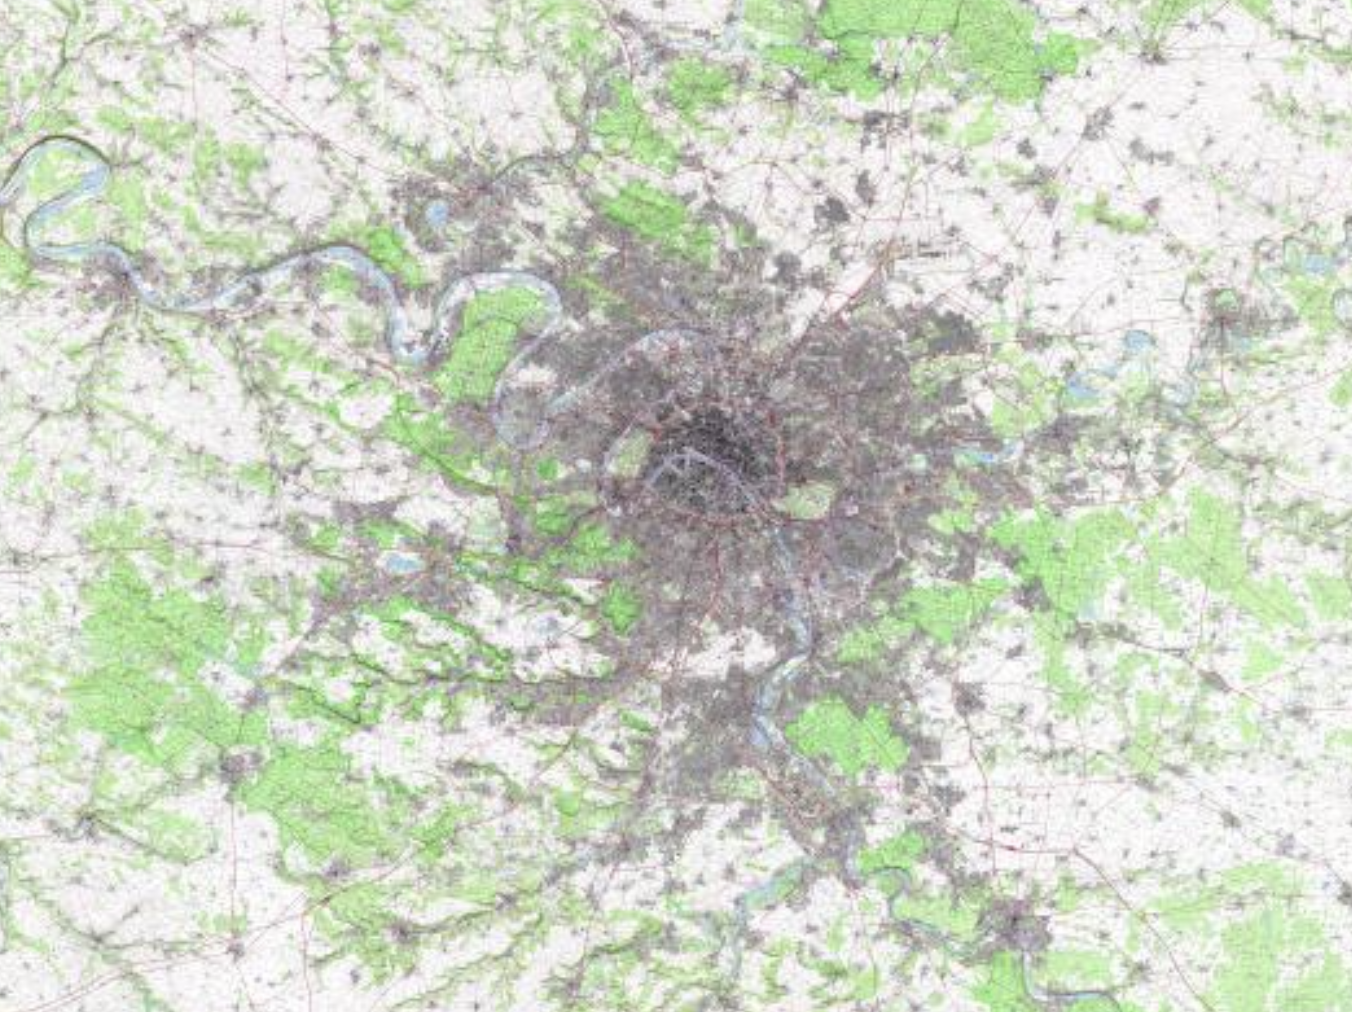
\includegraphics[width=0.9\textwidth]{figures/intro_bp}

\footnotesize\textit{Source: Geoportail}
}


\sframe{Modeling urban growth and land-use change}{

%  Understanding drivers of urban growth and land-use change at the metropolitan scale often requires to isolate and estimate stylized processes of urban evolution. Several land-use change and urban growth models for example based on cellular automata have been introduced in the literature, but their lack of generality and need for rich data may become a shortcoming.

$\rightarrow$ Cellular automata models or models of land-use change generally highly data-driven

\medskip

$\rightarrow$ May be case-specific or conclusions difficult to generalize (see Sleuth for example \cite{clarke2007decade})

\medskip

$\rightarrow$ Issues to calibrate and validate these models \cite{engelen2008validating}

%calibration/validation + map comparison

%\cite{zhou2018gini} urban form / emissions

\bigskip

\textbf{Urban morphogenesis models approach:}

\smallskip

$\rightarrow$\textit{At the crossroad between Urban Simulation and Artificial Life, stylized models of urban growth processes}

\medskip

$\rightarrow$\textit{Importance of parsimony: generative modeling as a tool to understand processes}

}

\sframe{Contribution}{

%  We propose here to apply and calibrate a simple model of urban growth based on reaction-diffusion processes for population density, providing a rather general insight into world urban areas from simple data. 

% We significantly extend these result by (i) applying the model on the 1000 largest urban areas of the Global Human Settlements database \citep{Florczyk2019ghs}; (ii) proceeding to a calibration on three successive time windows (1975-1990, 1990-2000 and 2000-2015) what provides dynamical values for parameters; (iii) using genetic optimization algorithms to minimise the distance on morphological indicators for each area.

$\rightarrow$ Explore a simple model to capture morphogenesis based on abstract representation of urban processes; test their ability to reproduce existing urban systems.

\bigskip

$\rightarrow$ The simple reaction-diffusion model of urban growth is calibrated worldwide using GHSL, and in time.

\bigskip

$\rightarrow$ Globally comparable insights into processes of concentration and dispersion.

}





\section{Reaction-diffusion model}


\sframe{A simple Reaction-diffusion model}{


% This four-parameter model introduced by \cite{raimbault2018calibration} combines aggregation forces (positive externalities) with dispersal forces (negative externalities) to capture dynamics of urban form. The model was previously only simulated on synthetic initially empty spaces and statically calibrated by comparing the projection of final simulated configurations in a space of urban morphology indicators (Moran index, entropy, average distance, hierarchy) to real measures computed on a fixed-size moving window for Europe.


\justify

$\rightarrow$ Crucial role of the interplay between concentration forces and dispersion forces~\cite{fujita1996economics} in keeping Urban Systems at the border of chaos

\bigskip

$\rightarrow$ Potentiality of aggregation mechanisms (such as Simon model) to produce power laws \cite{dodds2017simon}

\bigskip

$\rightarrow$ Link with Reaction-diffusion approaches in Morphogenesis~\cite{turing1952chemical}

\bigskip

$\rightarrow$ Extension of a DLA-type model introduced by \cite{batty1991generating}, with simple abstract processes of population aggregation and diffusion

\bigskip
\bigskip


\textit{Raimbault, J. (2018). Calibration of a density-based model of urban morphogenesis. PloS one, 13(9), e0203516.}


}

\sframe{Model formalization}{

$\rightarrow$ Grid world with cell populations $\left(P_i\left(t\right)\right)_{1\leq i\leq N^2}$.

\bigskip

$\rightarrow$ At each time step:


\begin{enumerate}
\item Population growth with exogenous rate $N_G$, attributed independently to a cell following a preferential attachment of strength $\alpha$
\item Population is diffused $n_d$ times with strength $\beta$
\end{enumerate}

\bigskip

$\rightarrow$ Stopping criterion: fixed maximal population $P_m$.

%To avoid bord effects such as reflecting diffusion waves, border cells diffuse their due proportion outside of the world, implying that the total population at time $t$ is strictly smaller than $N_G\cdot t$.

\bigskip

$\rightarrow$ Output measured by morphological indicators: Moran index, average distance, rank-size hierarchy, entropy.


}



\sframe{Measuring urban morphology}{

\begin{enumerate}
\item Rank-size slope $\gamma$, given by $\ln \left( P_{\tilde{i}}/P_0\right) \sim k \textrm{ + } \gamma\cdot \ln \left(\tilde{i}/i_0\right)$ where $\tilde{i}$ are the indexes of the distribution sorted in decreasing order.
\item Entropy of the distribution:
\begin{equation}
\mathcal{E} \textrm{ = } \sum_{i=1}^{M}\frac{P_i}{P}\cdot \ln{\frac{P_i}{P}}
\end{equation}
$\mathcal{E}\textrm{ = }0$ means that all the population is in one cell whereas $\mathcal{E}\textrm{ = }0$ means that the population is uniformly distributed.
\item Spatial-autocorrelation given by Moran index, with simple spatial weights given by $w_{ij} \textrm{ = } 1/d_{ij}$
\[
I \textrm{ = } M \cdot \frac{\sum_{i\neq j} w_{ij} \left(P_i - \bar{P}\right)\cdot\left(P_j - \bar{P}\right)}{\sum_{i\neq j} w_{ij} \sum_{i}{\left( P_i - \bar{P}\right)}^2}
\]
\item Mean distance between individuals
\[
\bar{d} \textrm{ = } \frac{1}{d_M}\cdot \sum_{i<j} \frac{P_i P_j}{P^2} \cdot d_{ij}
\]
where $d_M$ is a normalisation constant
\end{enumerate}



}


\sframe{Model behavior (synthetic data))}{

\begin{center}

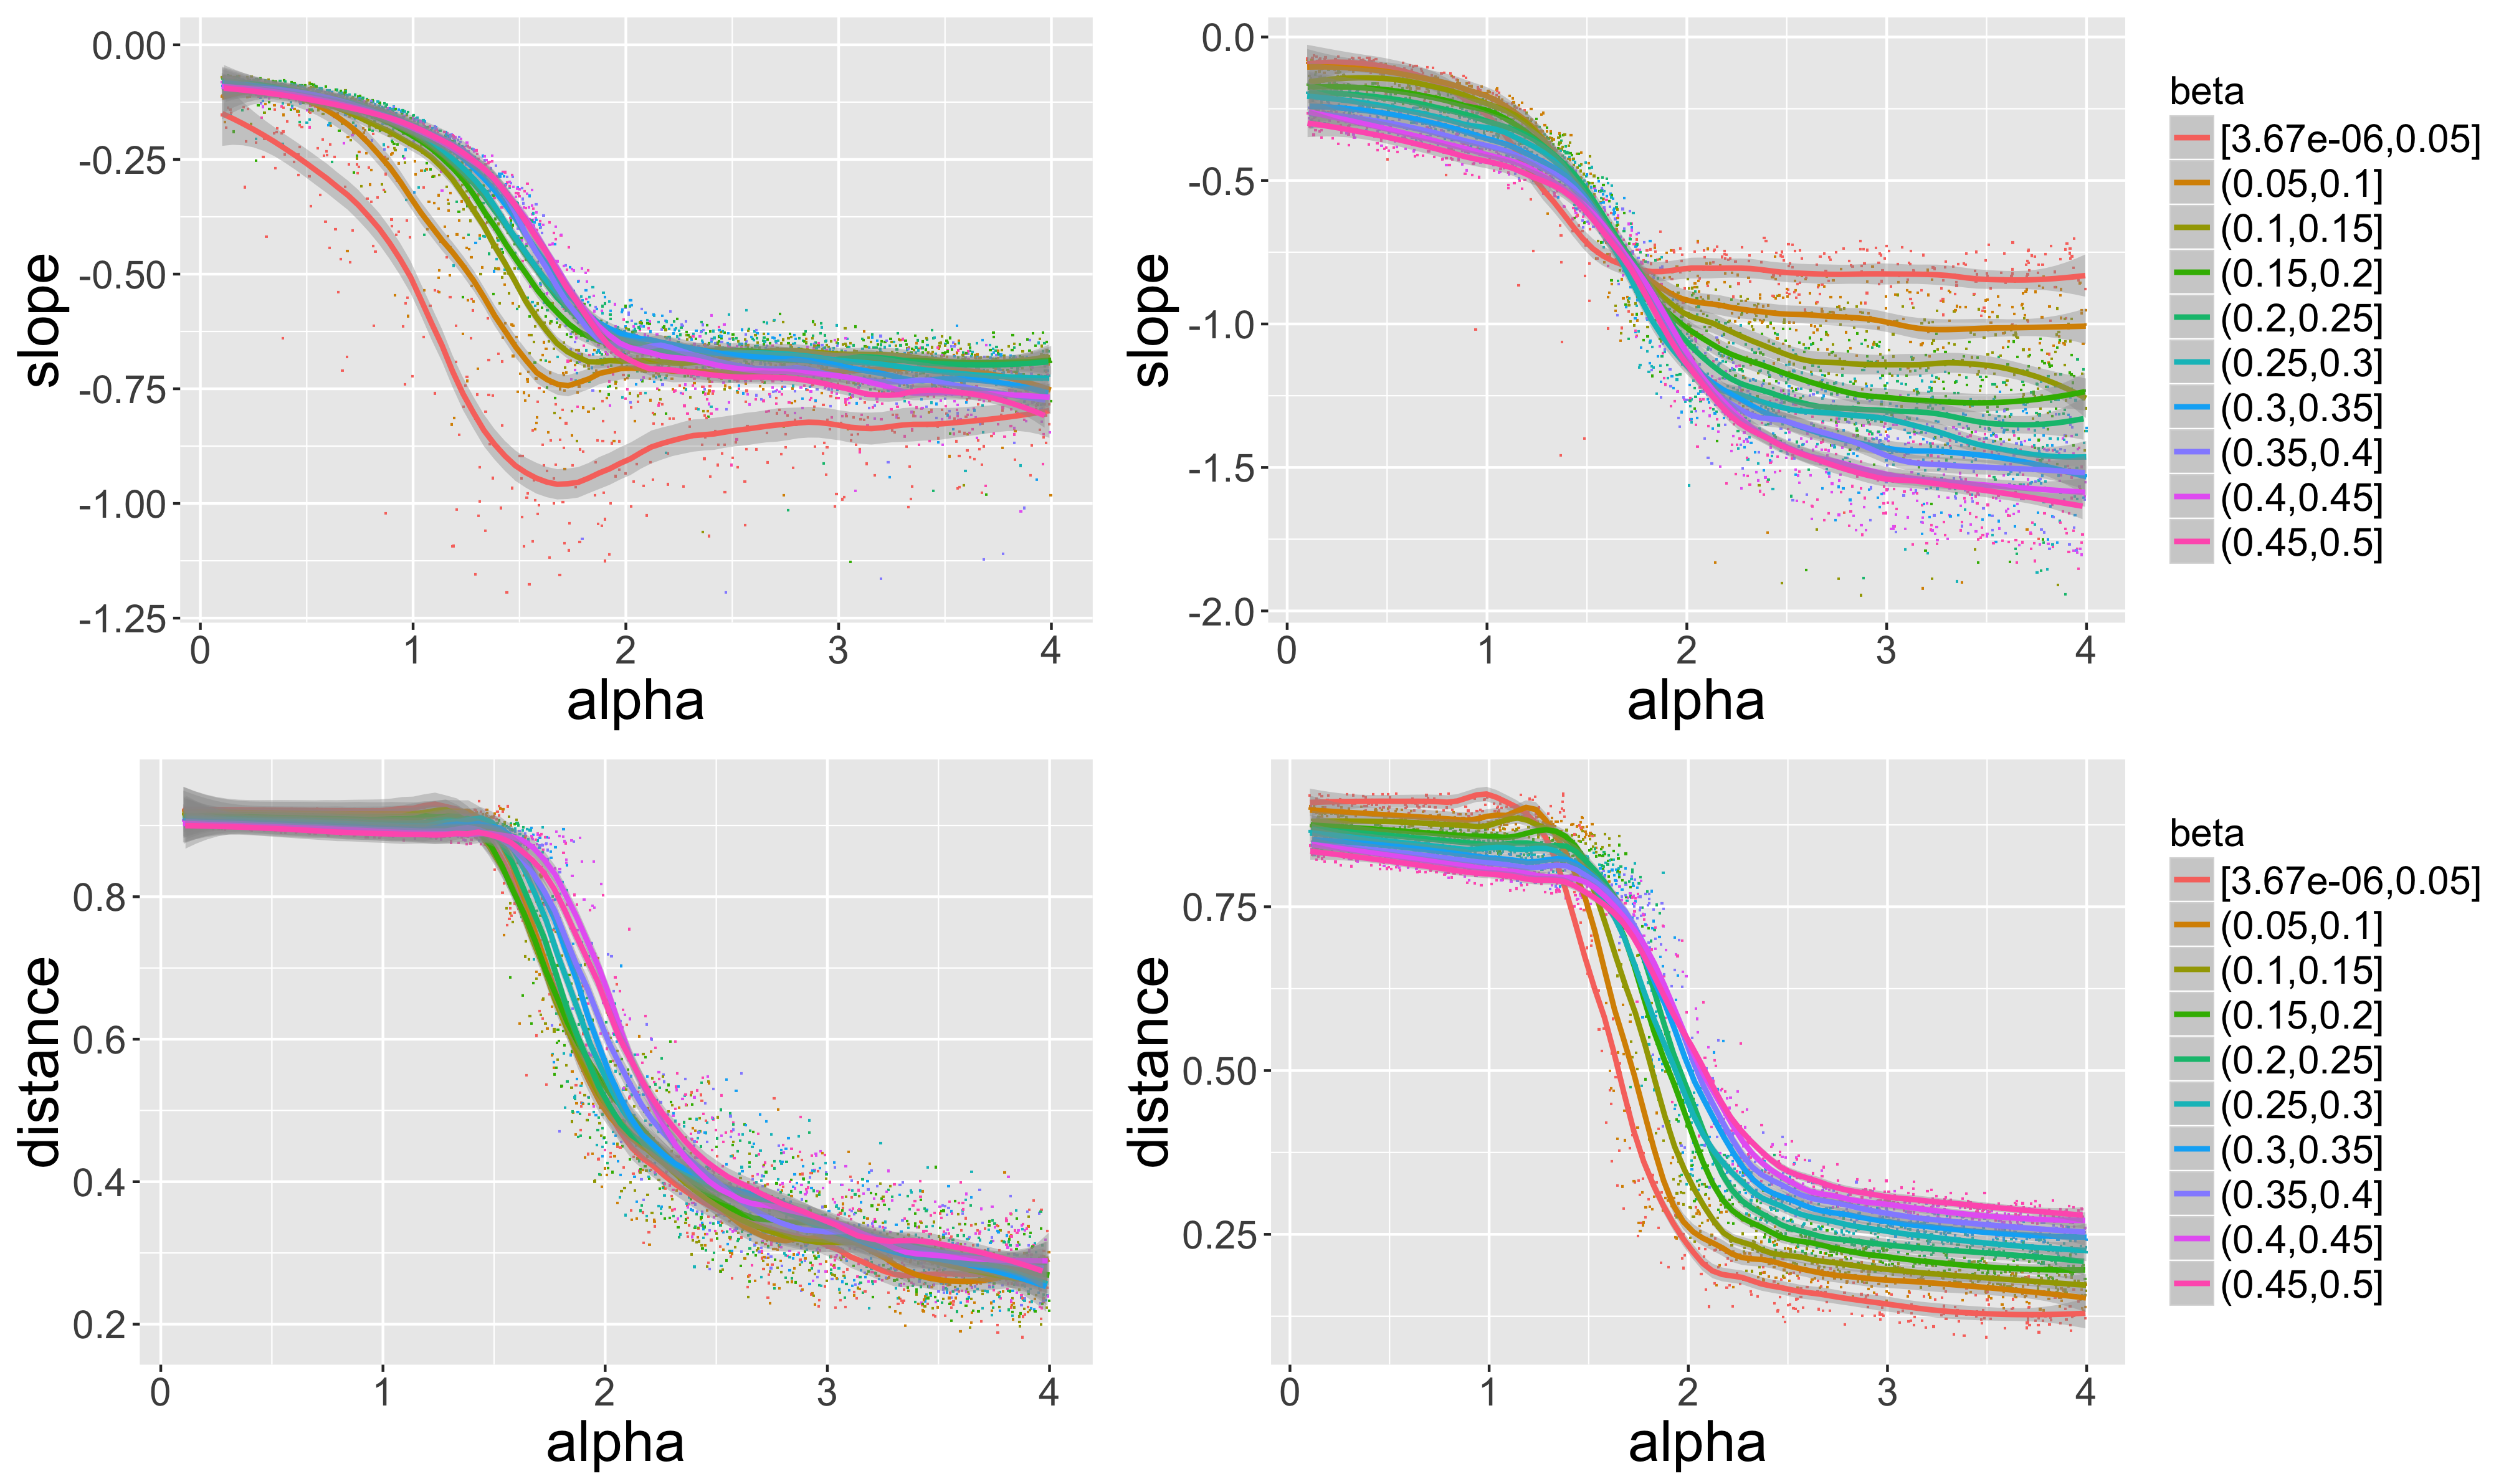
\includegraphics[width=0.9\textwidth]{figures/density_Fig3}

\end{center}

\footnotesize\textit{Phase transitions of indicators unveiled by exploration of the parameter space (80000 parameter points, 10 repetitions each)}


}


\sframe{Model application on a spatial grid}{

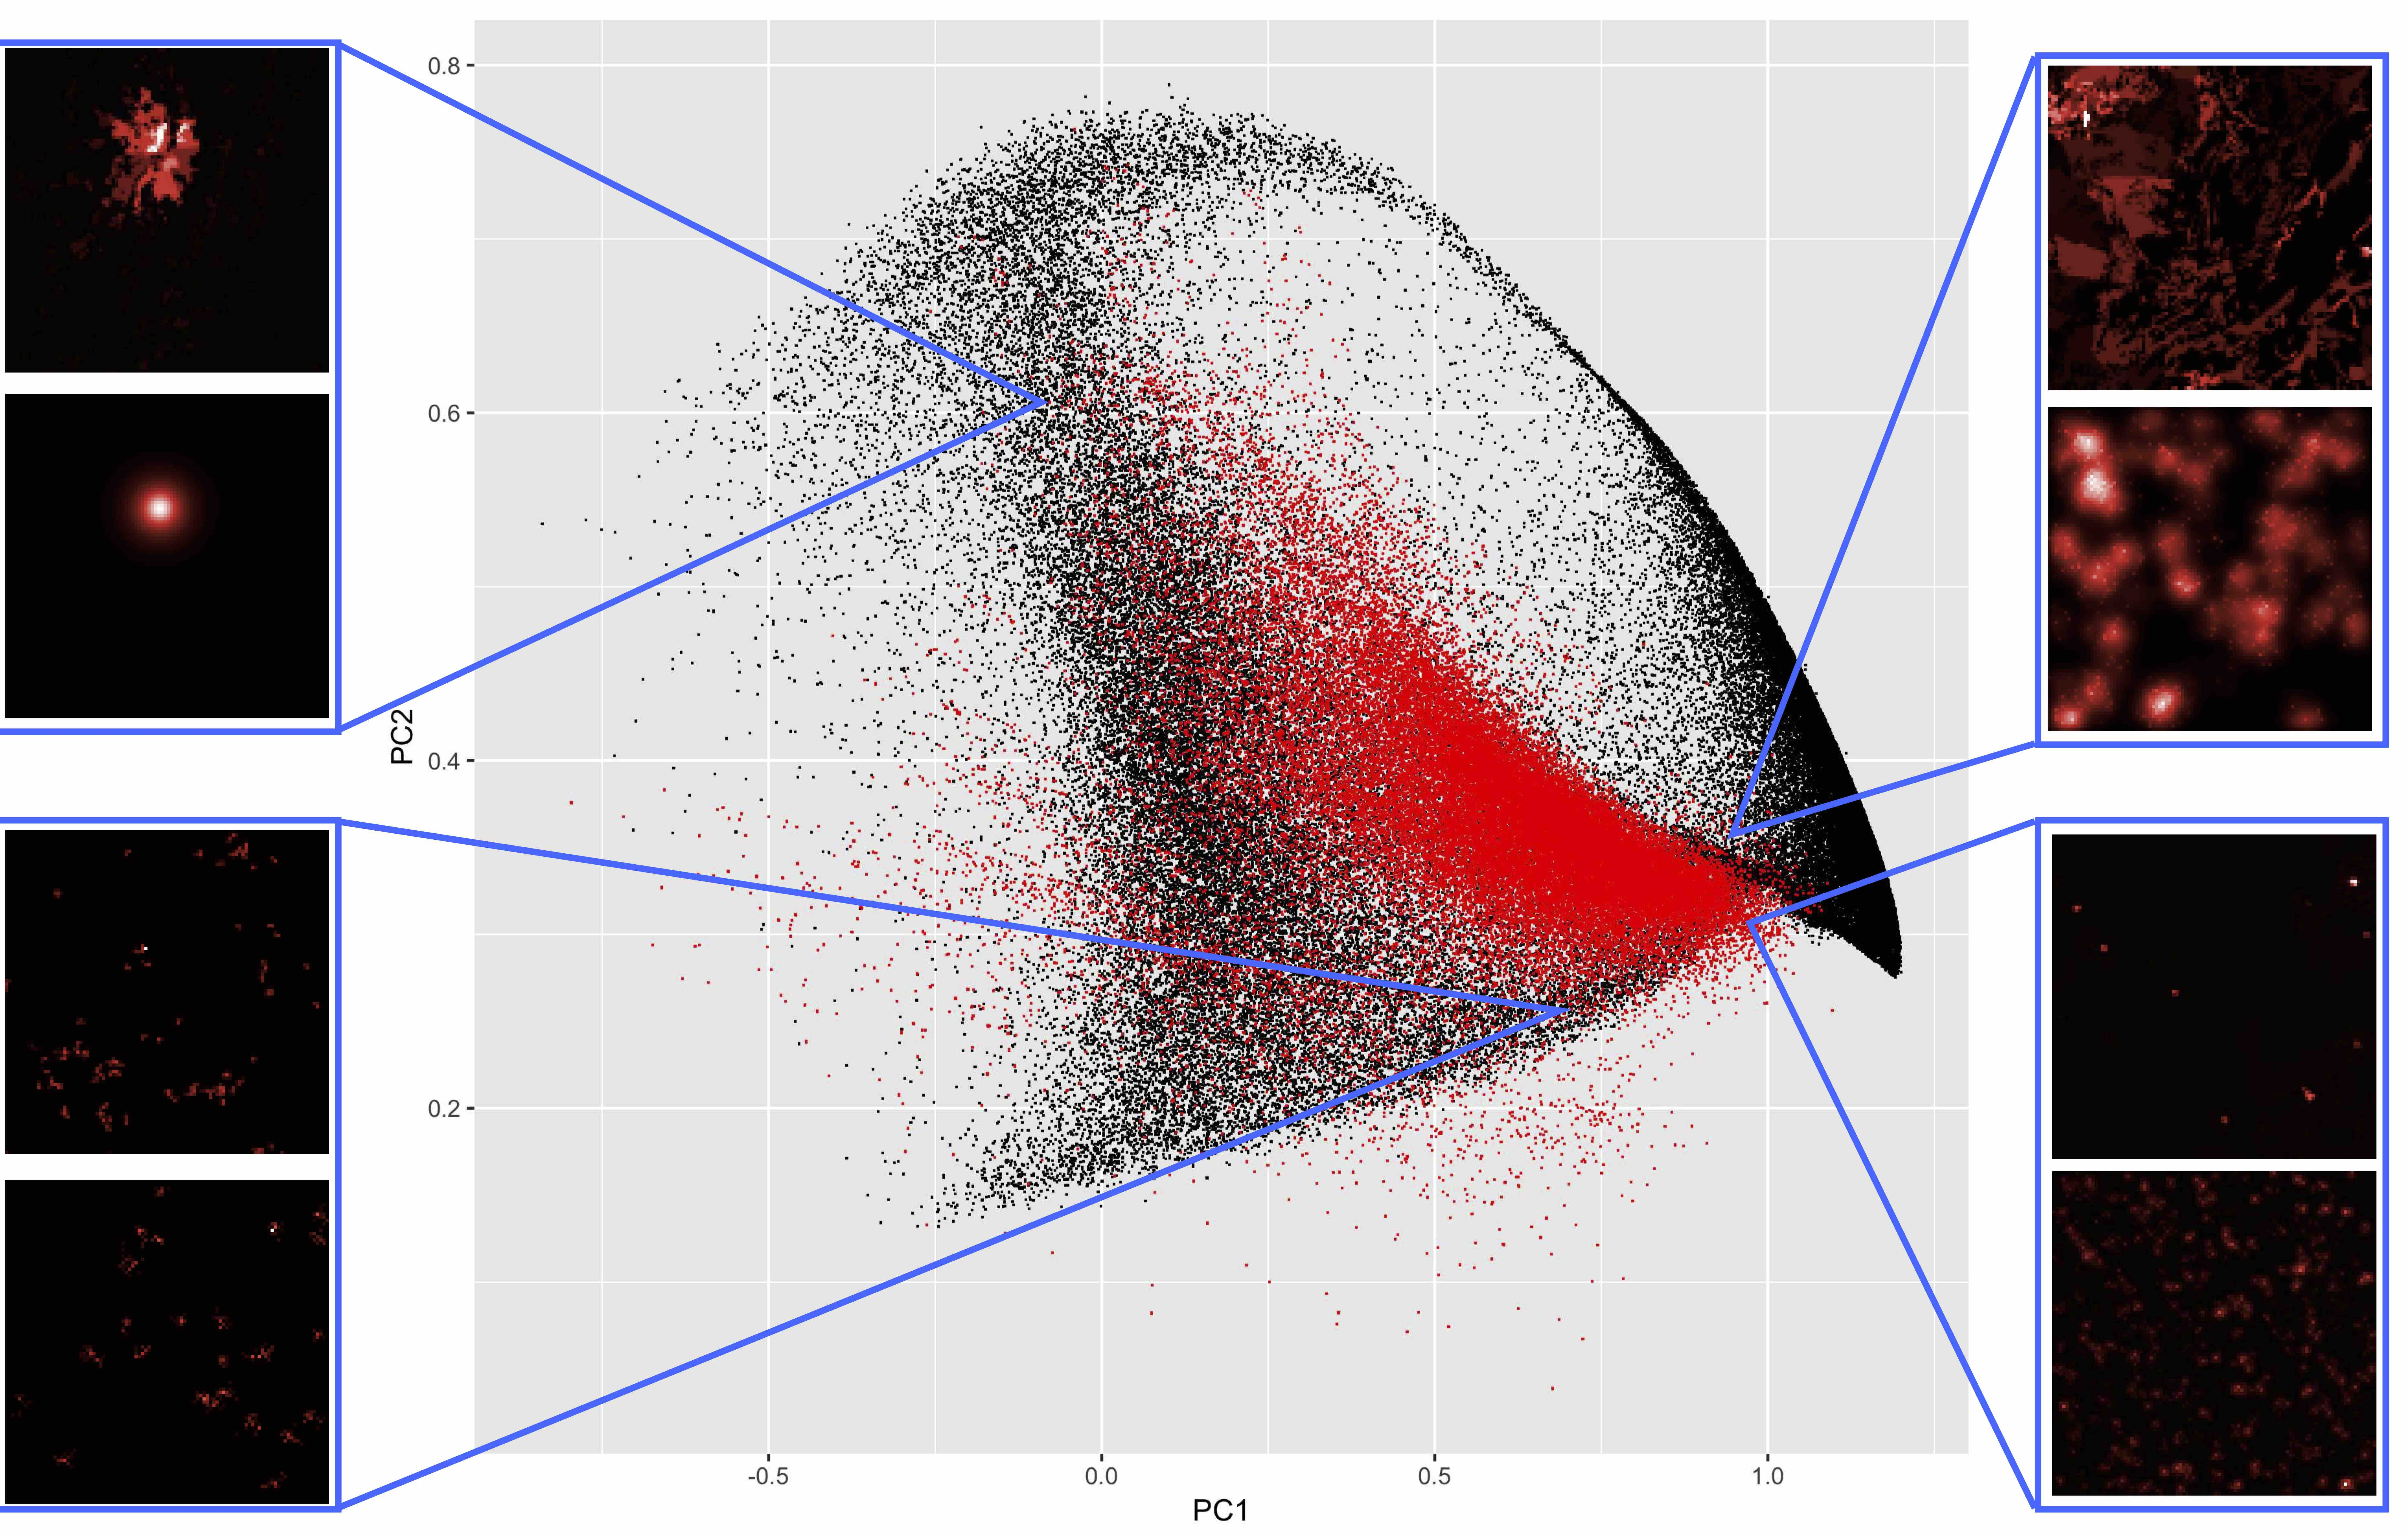
\includegraphics[width=0.9\textwidth]{figures/density_synth}

\footnotesize\textit{Brute force calibration by exploring the parameter space. Reproduction of most existing configuration in the morphological sense (here in principal plan).}

}



\section{Empirical analysis}

\sframe{GHSL database}{
	% brief description of GHSL; illustration

% + empirical approach: 1000 areas, window 0.25%

$\rightarrow$ Application on worldwide urban areas using the GHSL population grid

\medskip

$\rightarrow$ Dynamical calibration on three successive time windows (1975-1990, 1990-2000, 2000-2015)

\medskip

$\rightarrow$ Extraction of neighborhood (spatial span times 1.5) of 1000 larger urban areas (2015 population)

\medskip

$\rightarrow$ Computation of morphological indicators on corresponding population grids


}

\sframe{Global indicators distribution: Moran}{

\centering

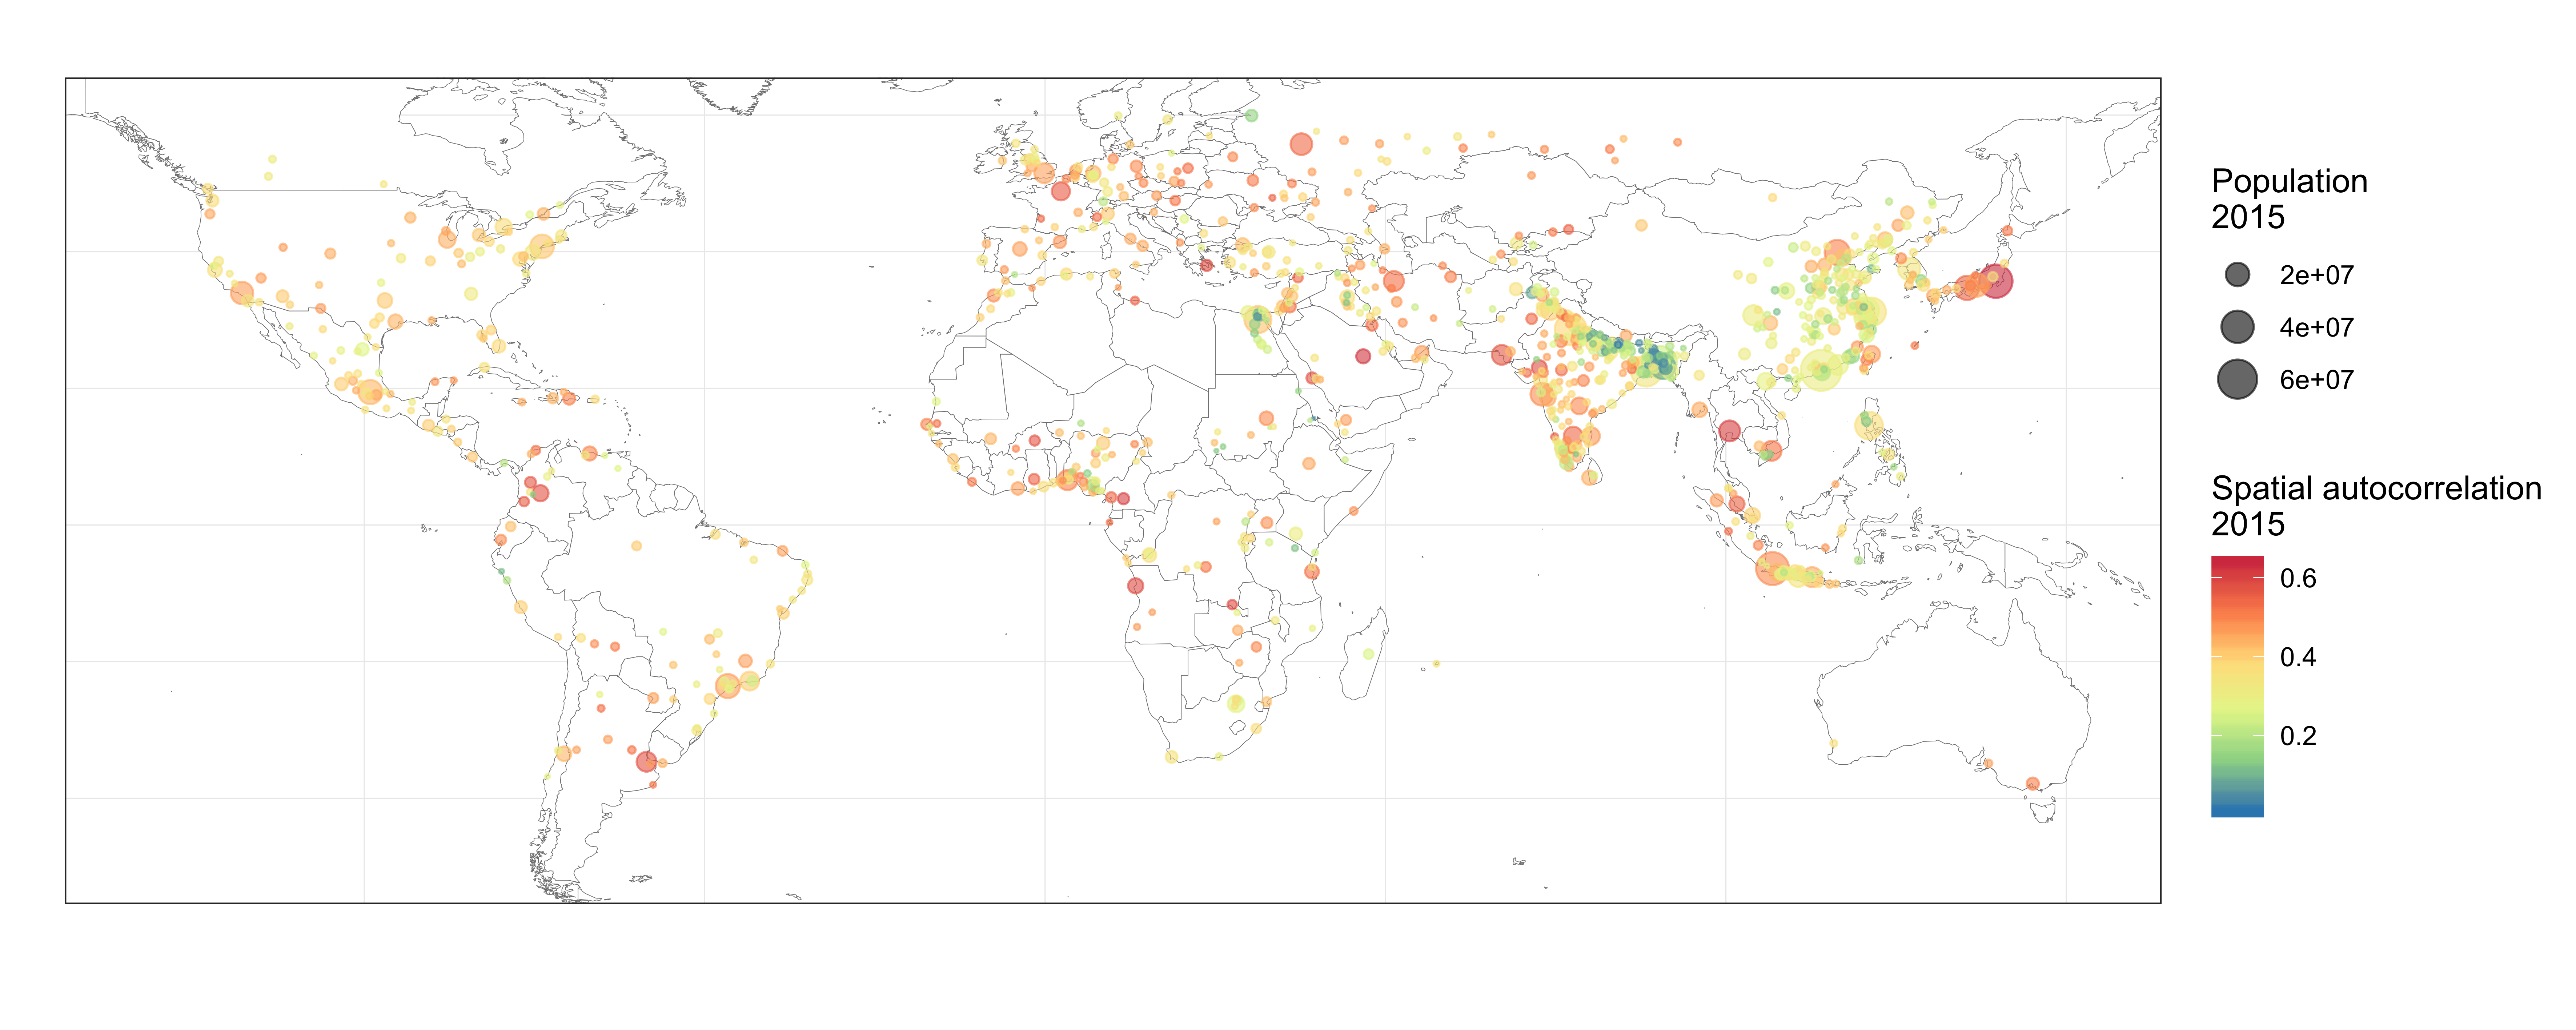
\includegraphics[width=\linewidth]{figures/mapindic_moran_2015.png}

\medskip

\small

\textit{Regional patterns for Moran index}

}

\sframe{Global indicators distribution: average distance}{

\centering

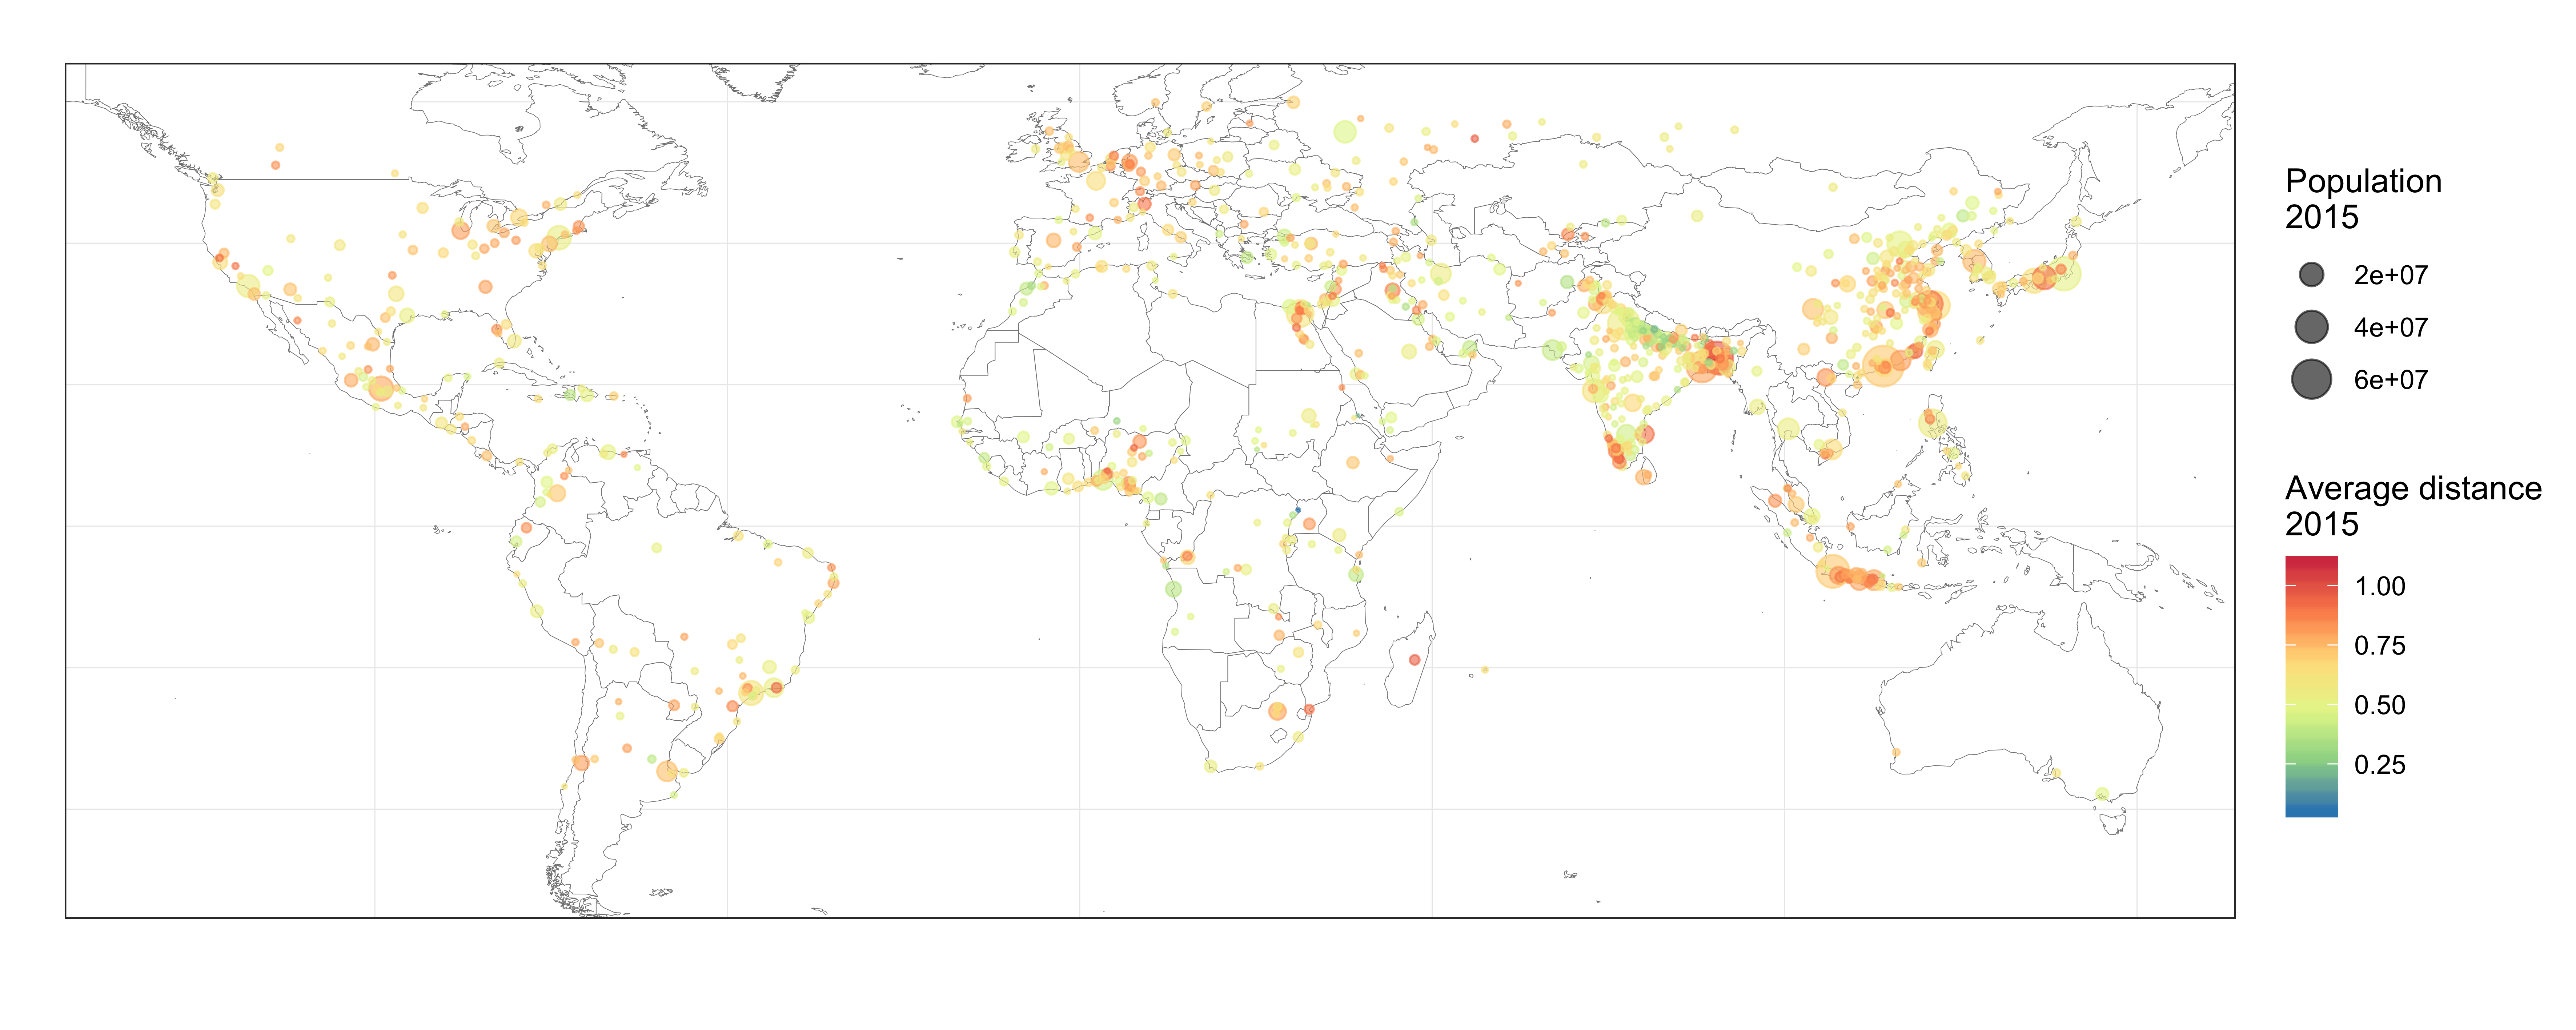
\includegraphics[width=\linewidth]{figures/mapindic_avgDist_2015.png}

\medskip

\small

\textit{Complementarity of average distance indicator}

}

\sframe{Clustering morphological trajectories}{

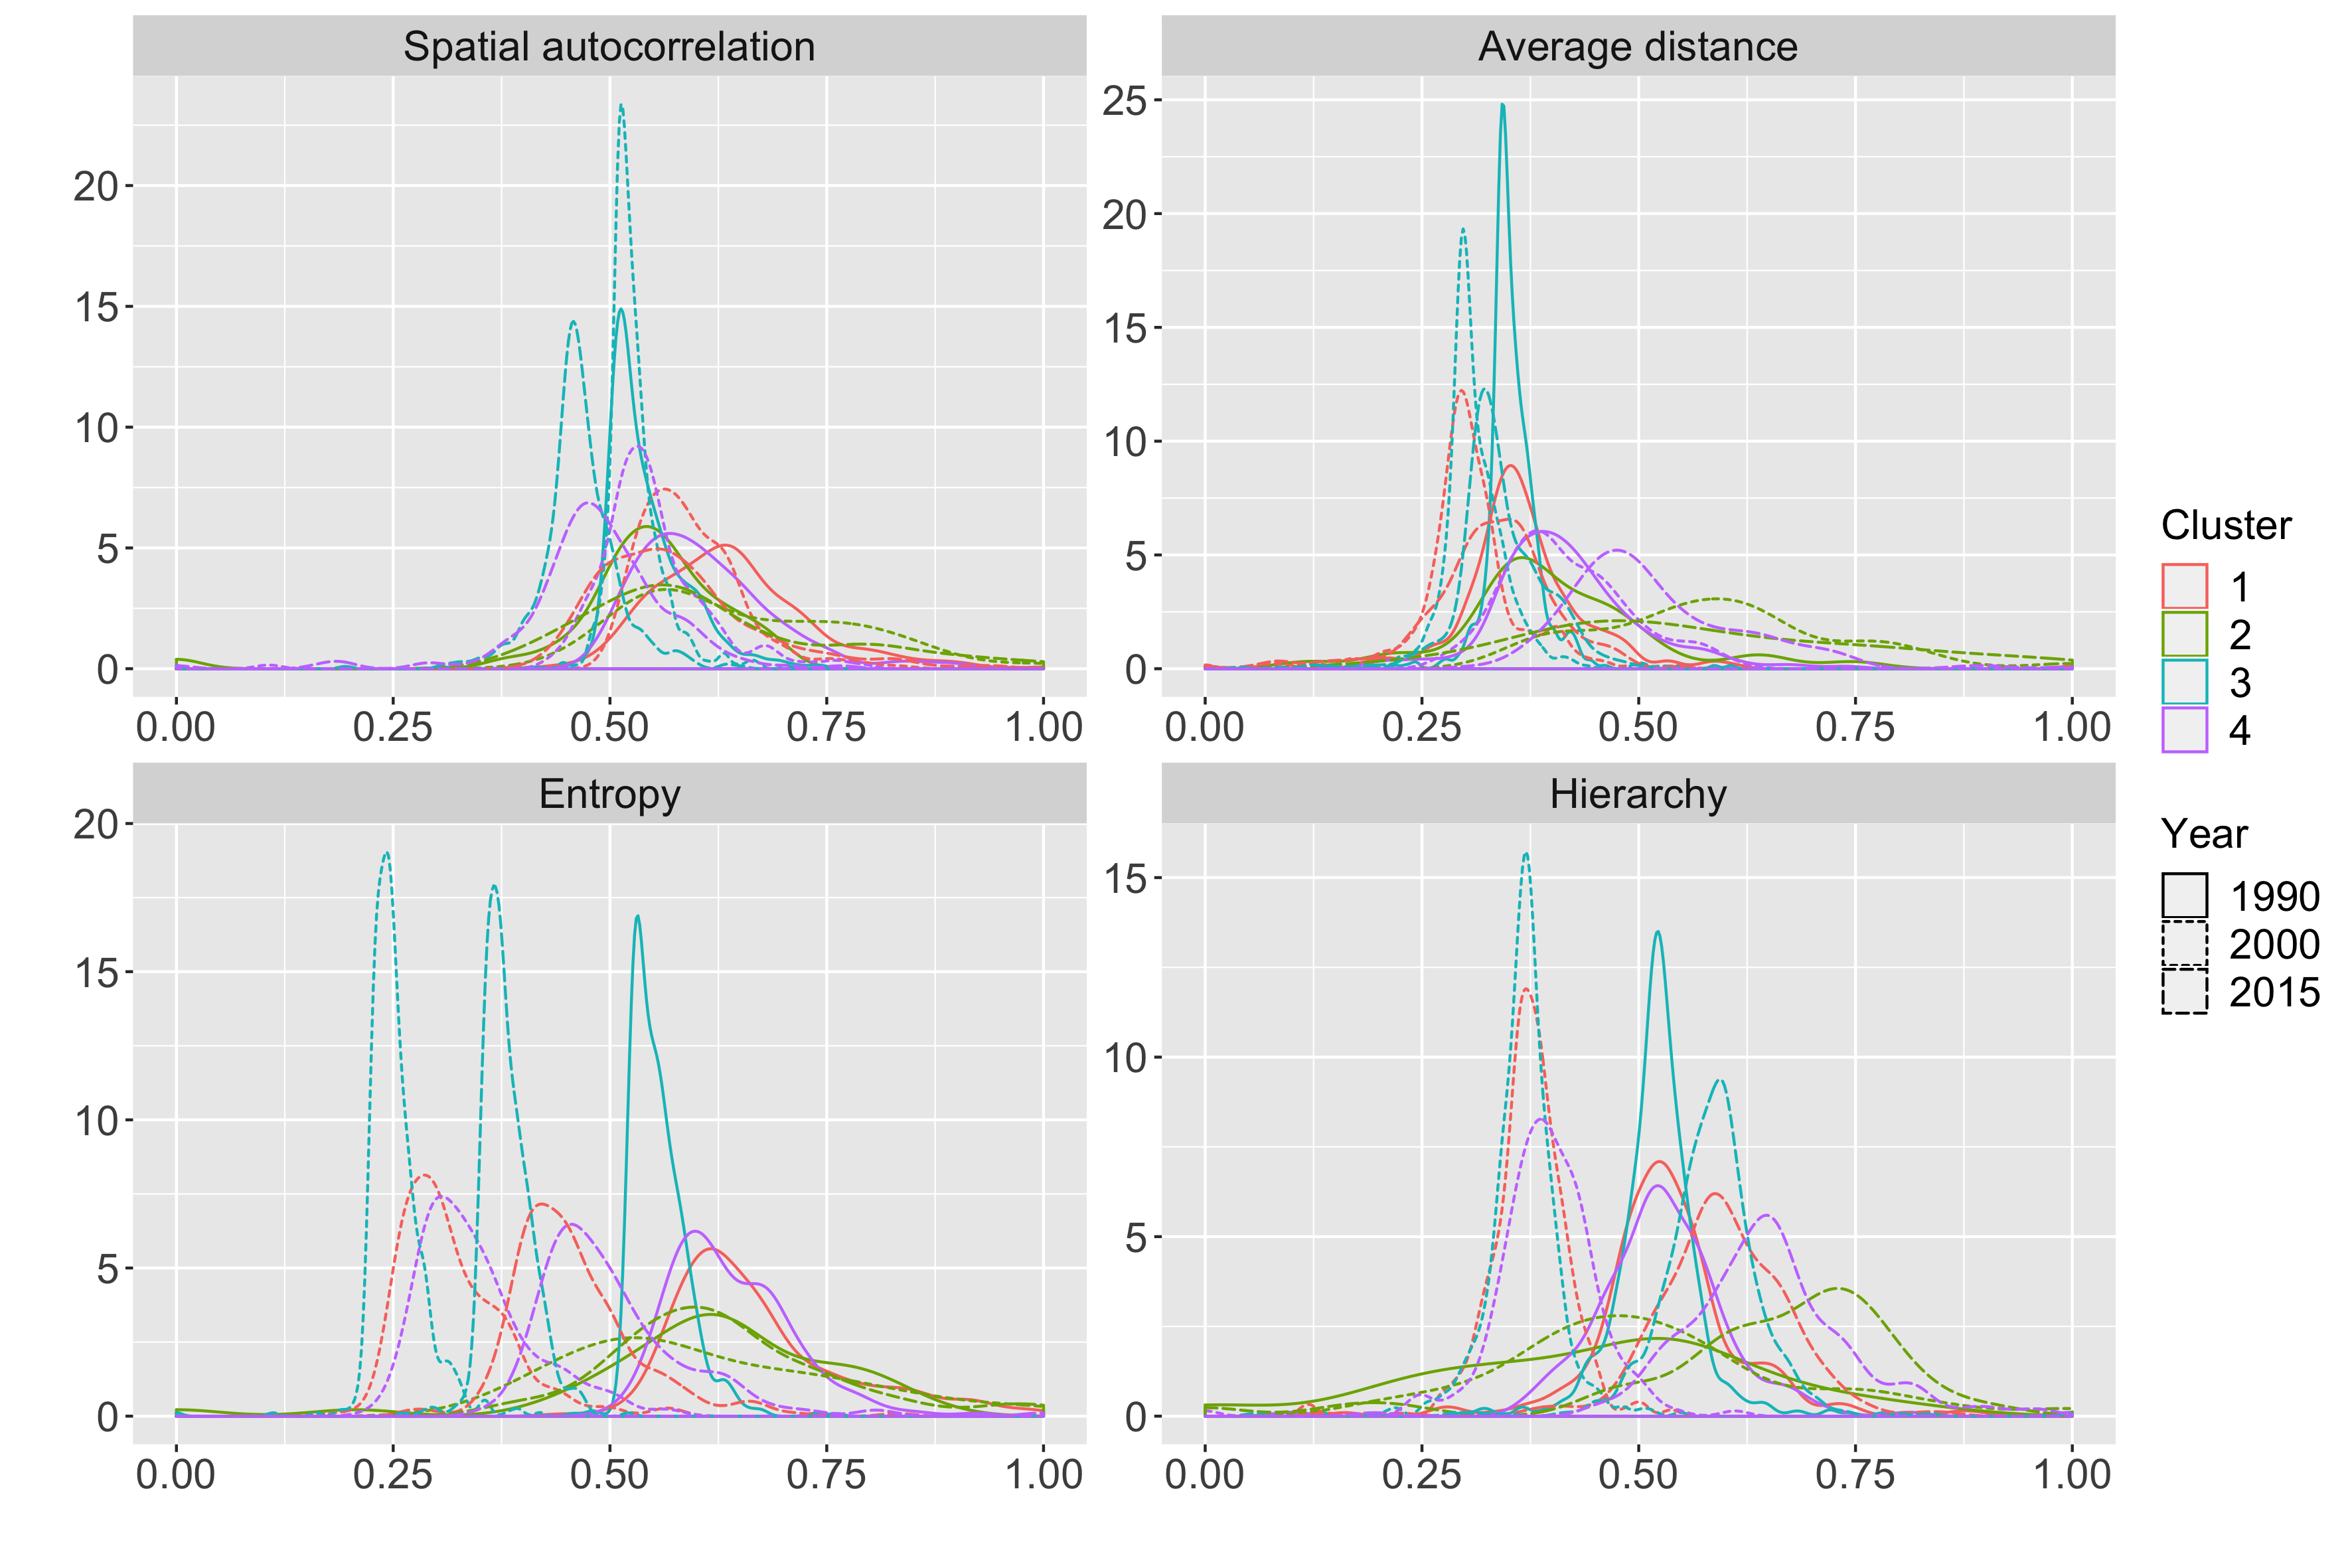
\includegraphics[width=0.55\textwidth]{figures/distributions_cluster-year.png}
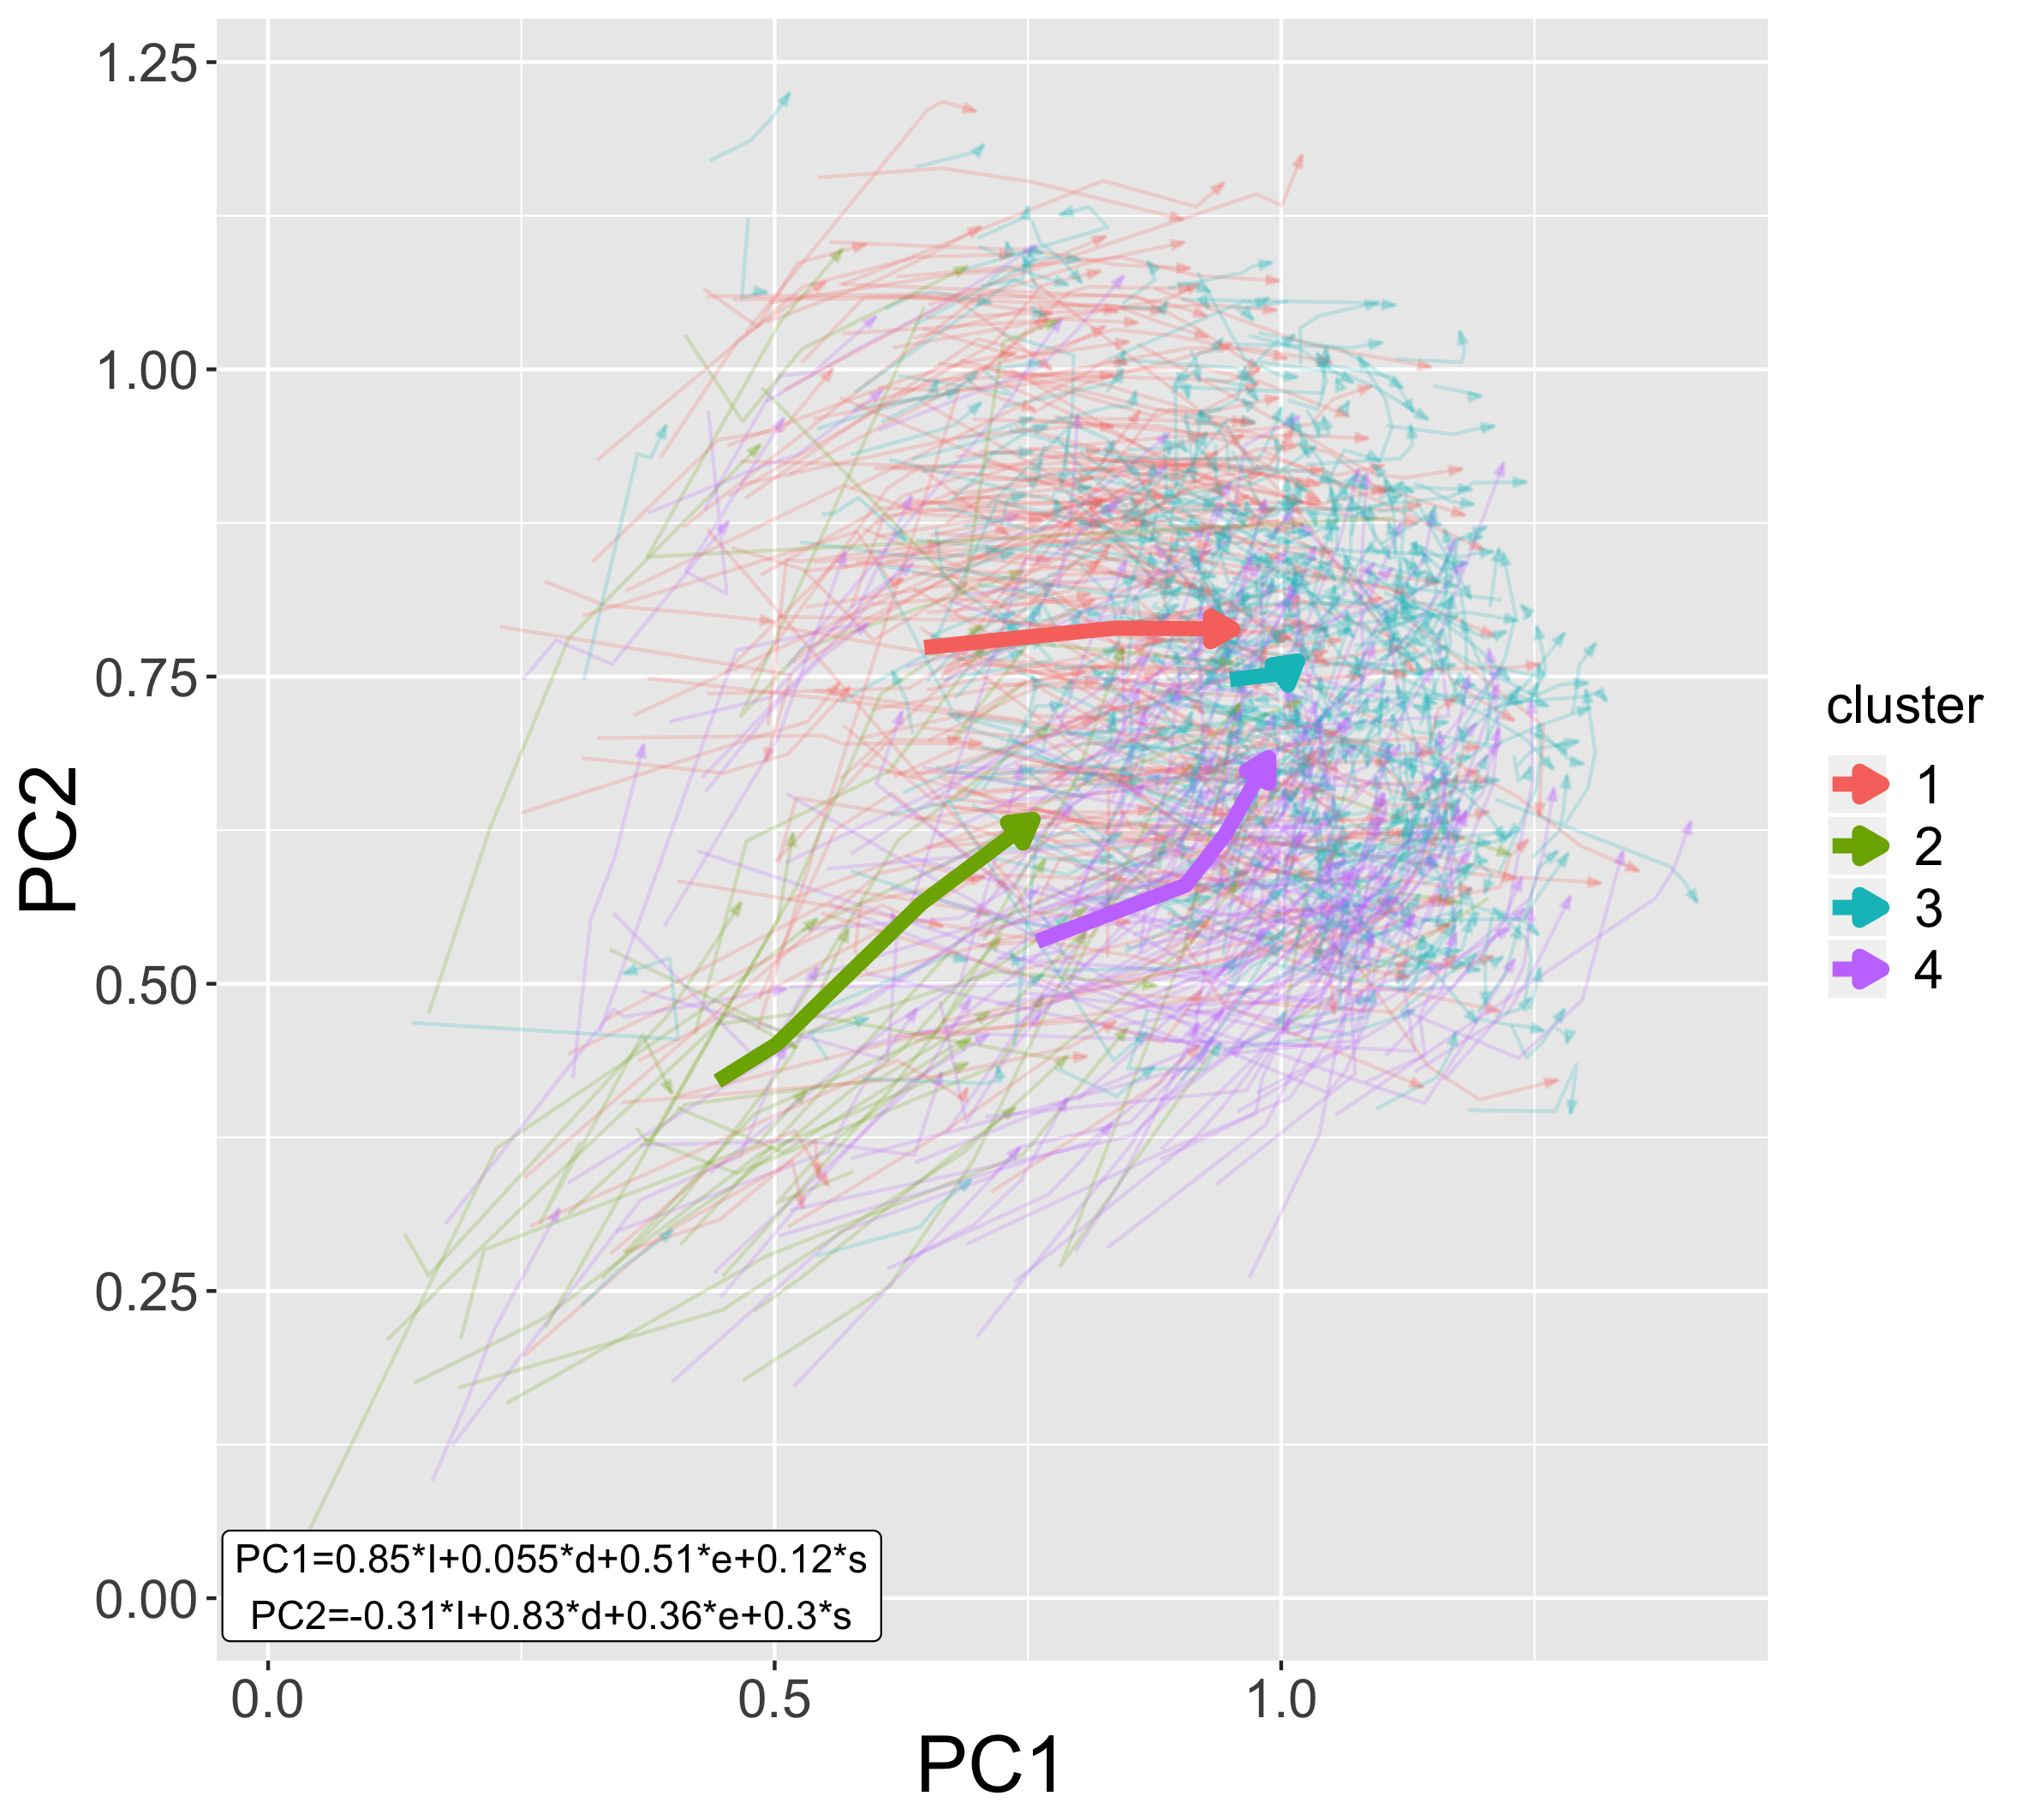
\includegraphics[width=0.4\textwidth]{figures/PCA_trajectories.png}

\medskip

\small

\textit{Disjoint distributions and temporal trajectories: model application is relevant}

}

\sframe{Distribution of clusters}{

\centering

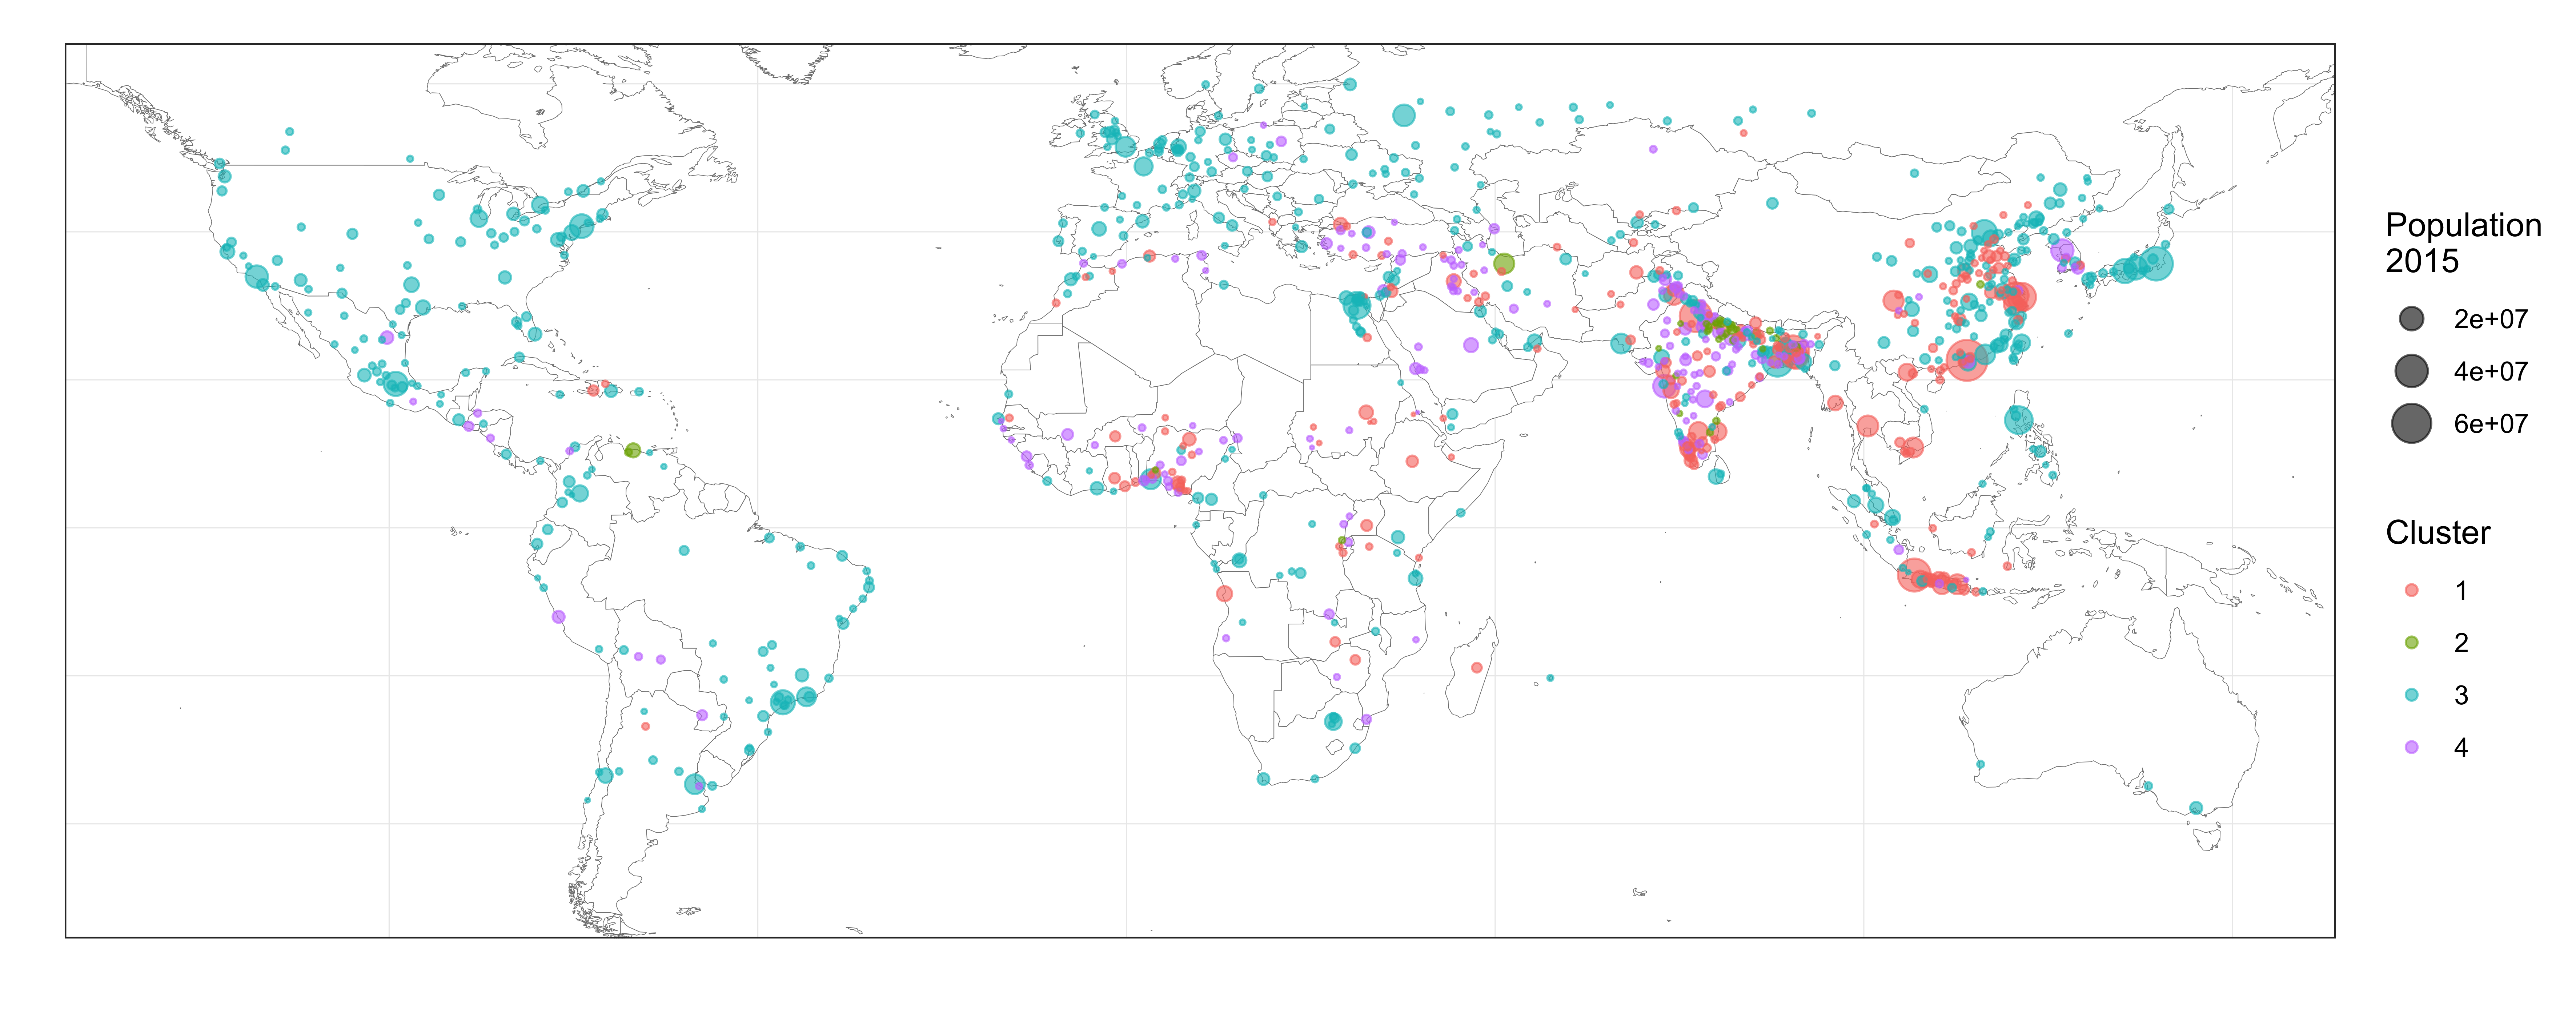
\includegraphics[width=\linewidth]{figures/mapindic_cluster.png}

}

\sframe{Correlations with urban area properties}{

\centering

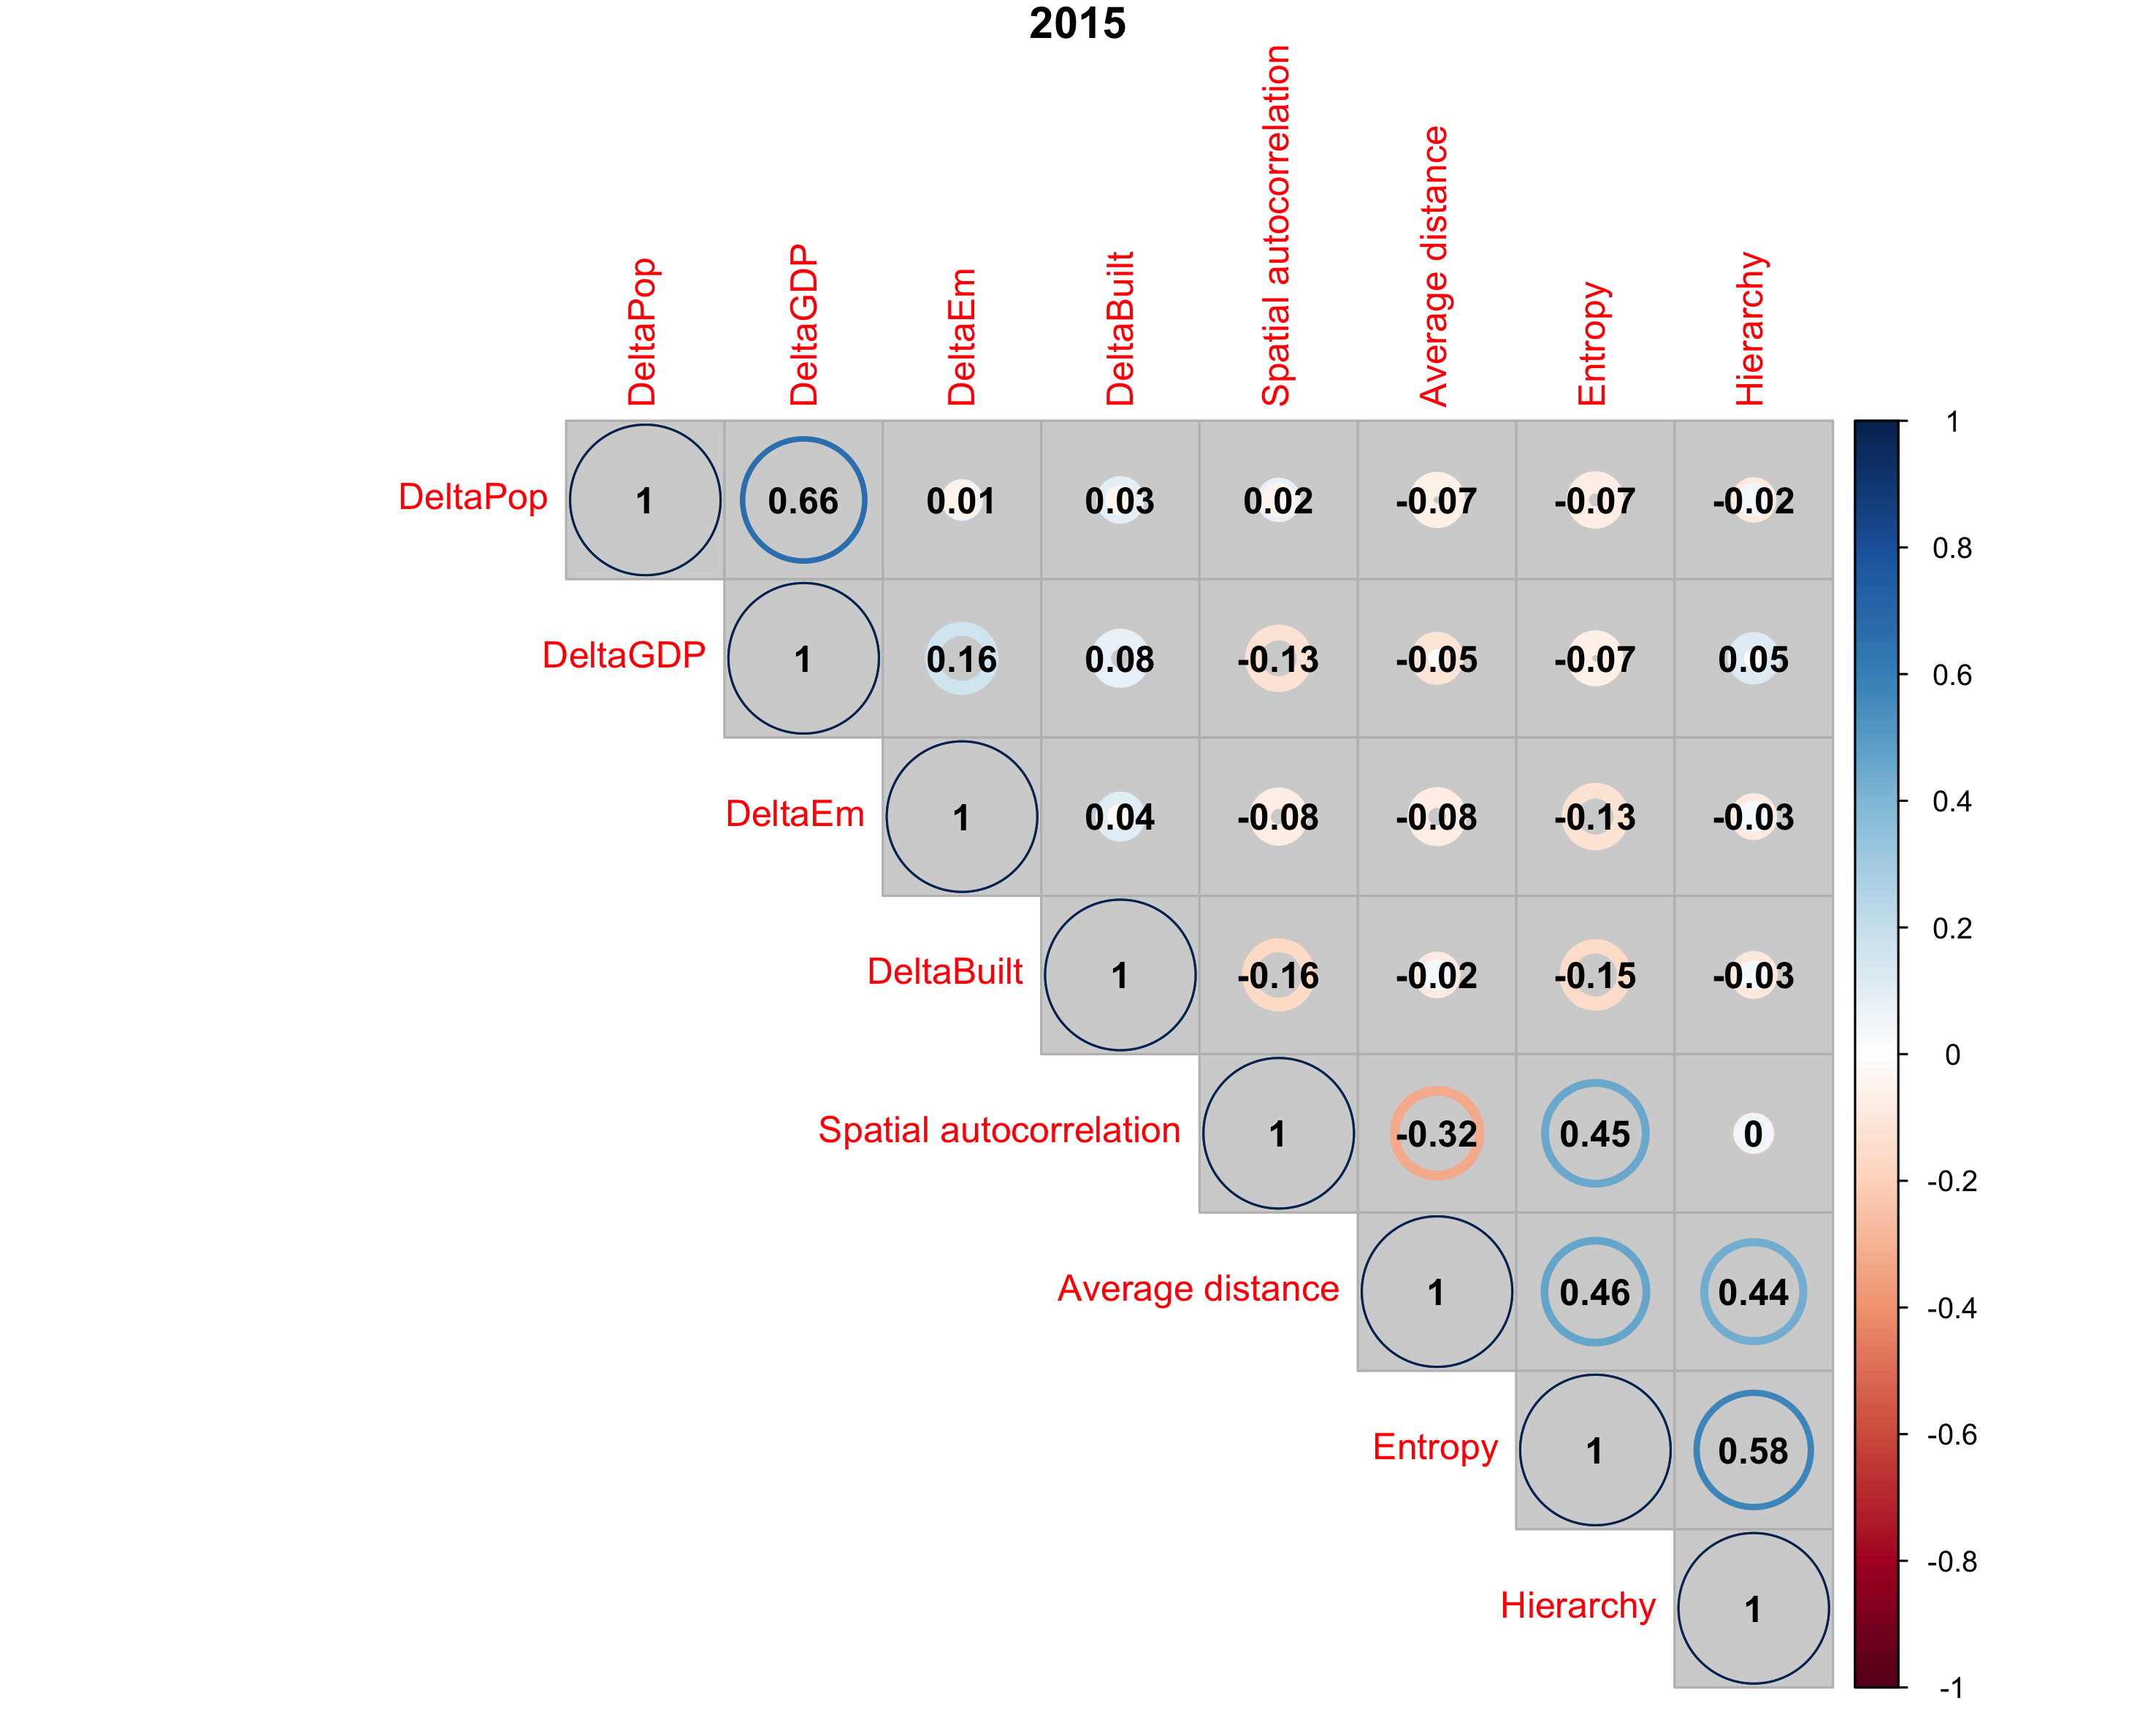
\includegraphics[trim={4cm 0 0 0},width=0.48\linewidth]{figures/correlations_deltavars-morpho_2015.png}
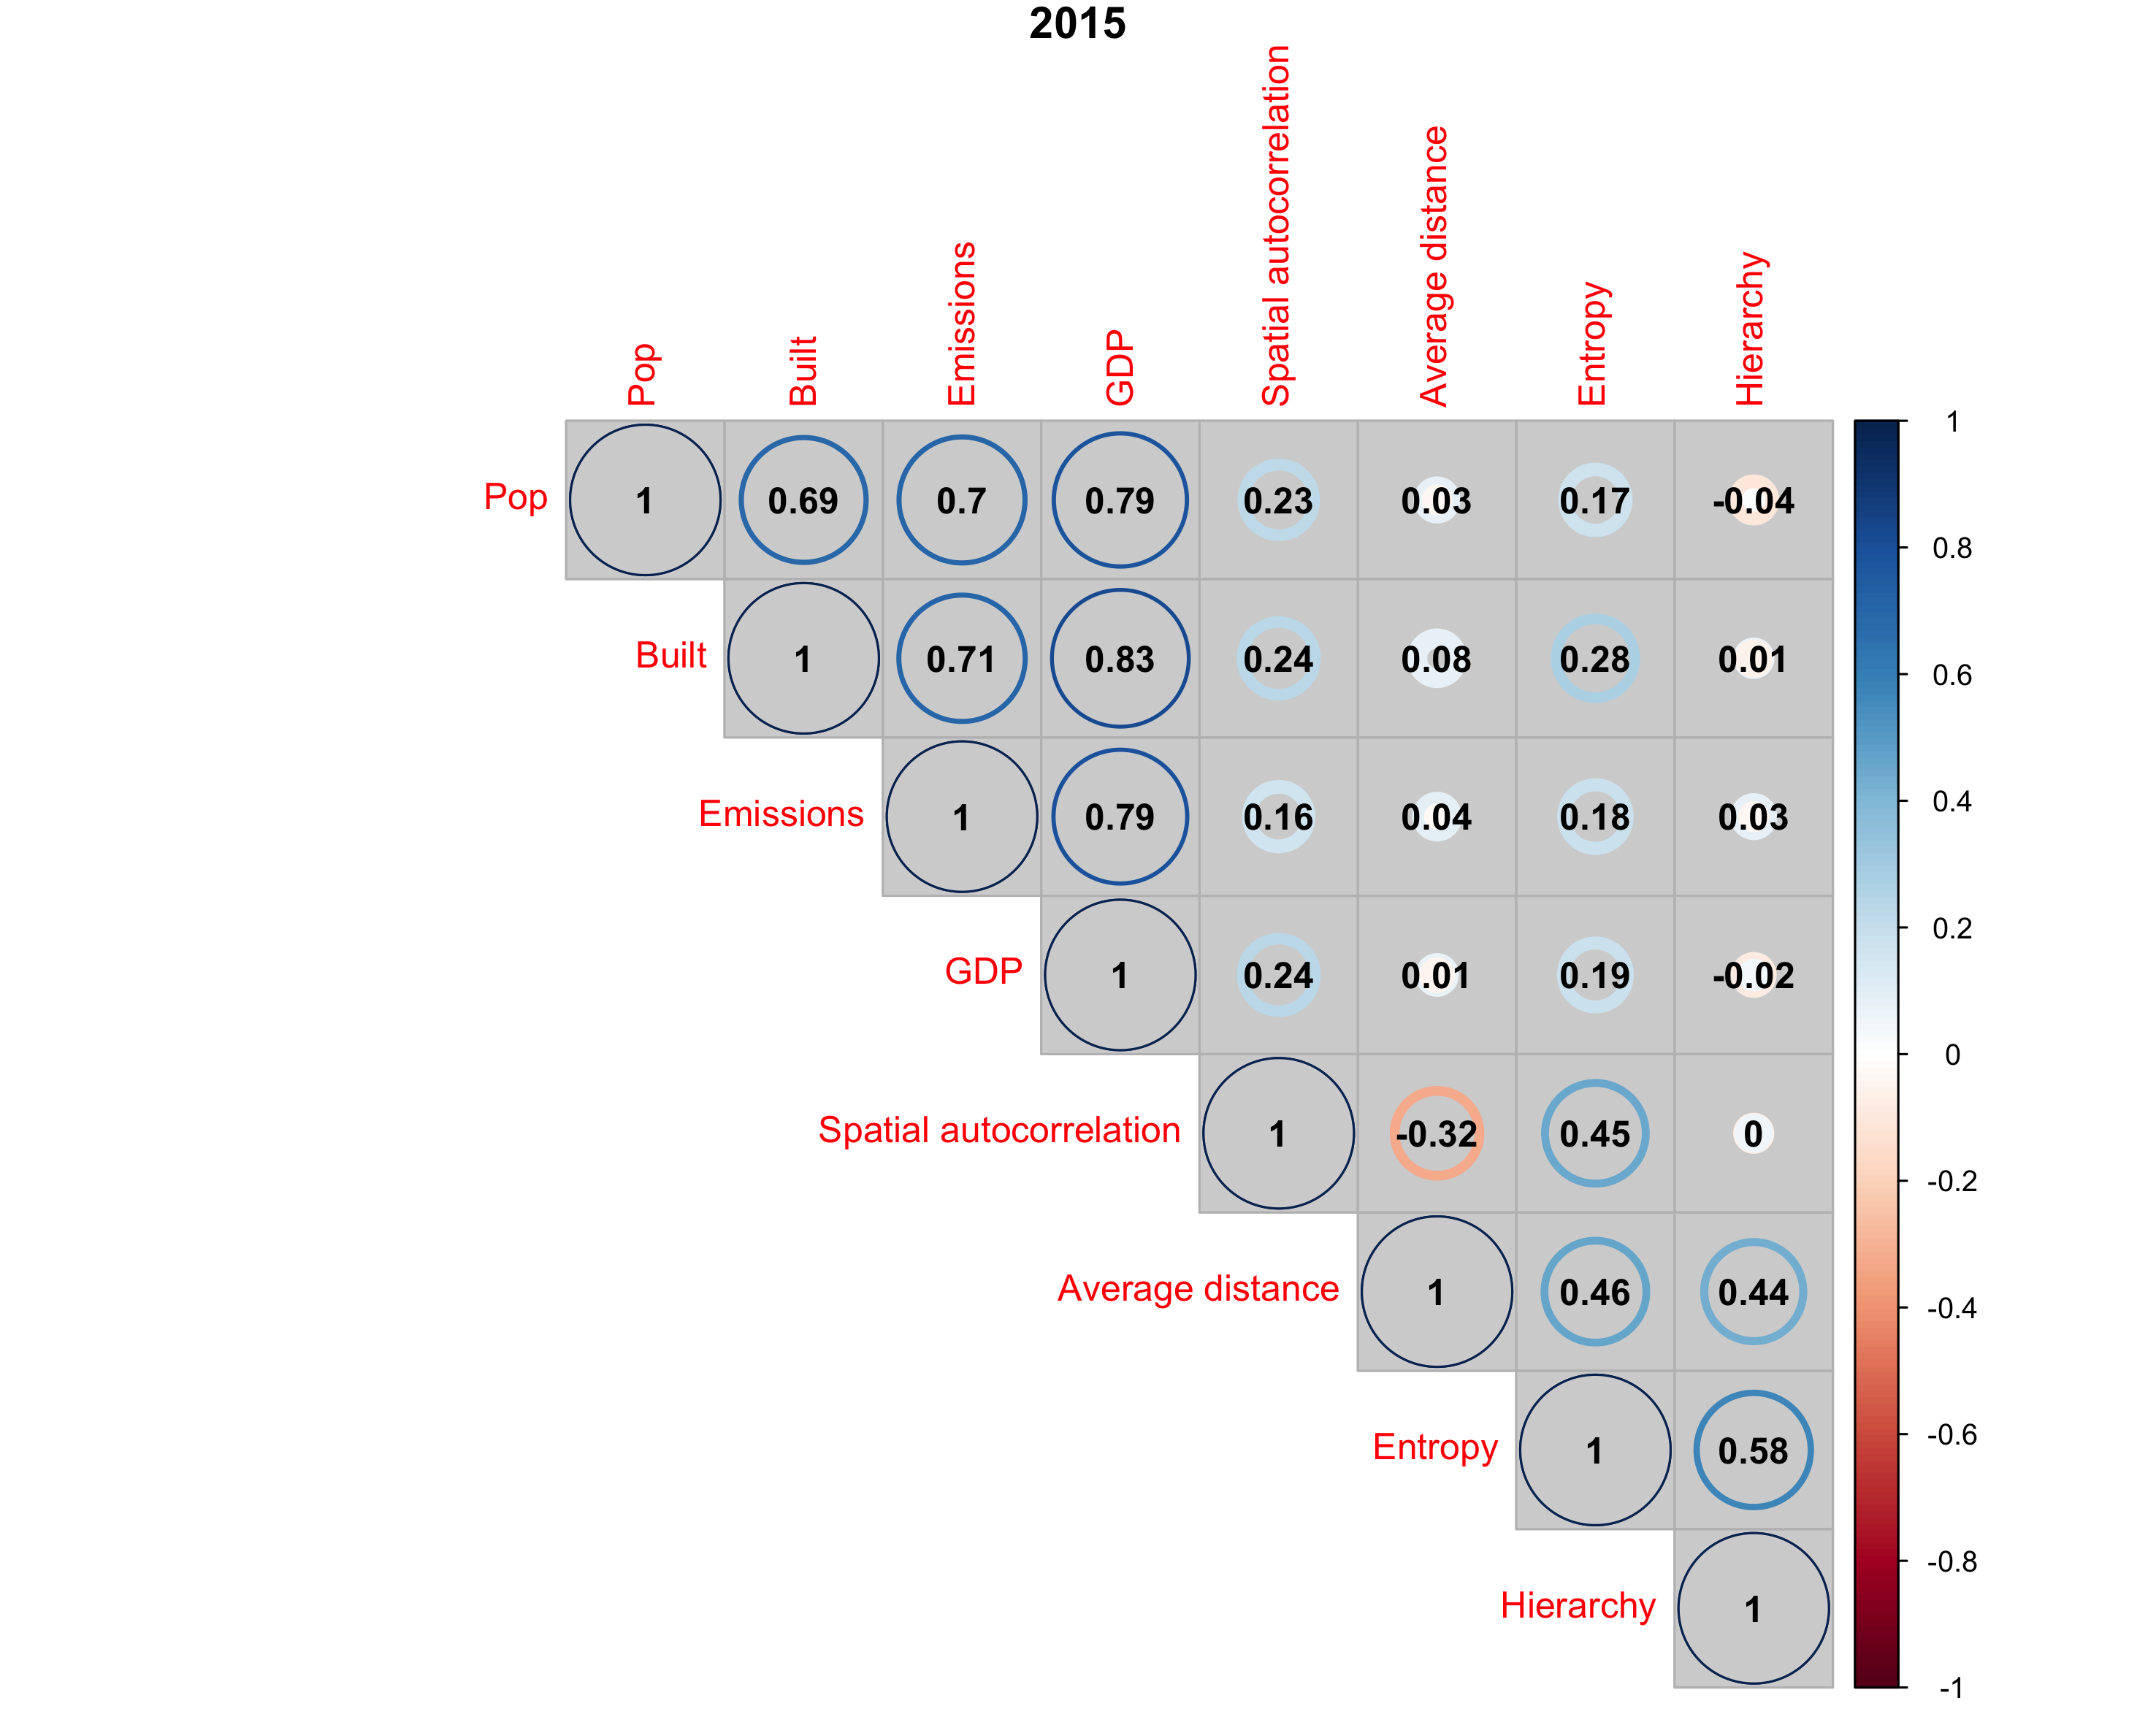
\includegraphics[trim={4cm 0 0 0},width=0.48\linewidth]{figures/correlations_vars-morpho_2015.png}

}




\section{Model calibration}

\sframe{Calibration method}{
 % setup, error
 

 
\begin{itemize}
	\item For a time period $\left[t_0,t_f\right]$, model initialized with population at $t_0$
	\item Growth rate $N_G$ is computed by constraining with actual population growth: $N_G \textrm{ = } \left(P_i\left(t_f\right) - P_i \left(t_0\right)\right) / T$ where $T$ is a calibration parameter
	\item Fitness functions: squared relative population error and squared relative morphological indicator error
	\item Biobjective genetic algorithm (NSGA2) run for each areas ($\sim 600$ areas large enough) and each time windows (1000 generations, population of 100), on parameters $\alpha, \beta, T$
\end{itemize}

 
}


\sframe{Implementation}{

% openmole slide

% The computational cost being high, results are obtained by using the OpenMOLE model exploration software \citep{reuillon2013openmole}, which provides in a transparent way the optimization algorithms and the distribution of calibrations on a computation grid.


%\footnotesize
\justify

\textit{Performance constraints: large number of calibration algorithms to be run}

\medskip

$\rightarrow$ model implemented in \texttt{scala} and integrated within the \texttt{spatialdata} library for spatial sensitivity analysis (including implementations of

\cite{raimbault2018indirect} \cite{raimbault2018calibration} \cite{favaro2011gibrat} \cite{cottineau2015modular})

See \url{https://github.com/openmole/spatialdata}

\medskip

$\rightarrow$ integration into the OpenMOLE model exploration open source software \cite{reuillon2013openmole}

\begin{center}

\includegraphics[height=0.13\textheight]{figures/iconOM.png}

\includegraphics[height=0.13\textheight]{figures/openmole.png}
\end{center}

%(X year of computation for the results presented here)

\footnotesize
\textit{Enables seamlessly (i) model embedding; (ii) access to HPC resources; (iii) exploration and optimization algorithms}

\medskip

%\textbf{Come to the satellite \textit{New Methods and Epistemologies to Explore Simulation Models} tomorrow afternoon in LHN-TR+05}

\textbf{Apply for the OpenMOLE summer school before January 15th}

\url{https://exmodelo.org/}

}

\sframe{Examples of results}{

% pareto fronts for two different areas

\begin{center}

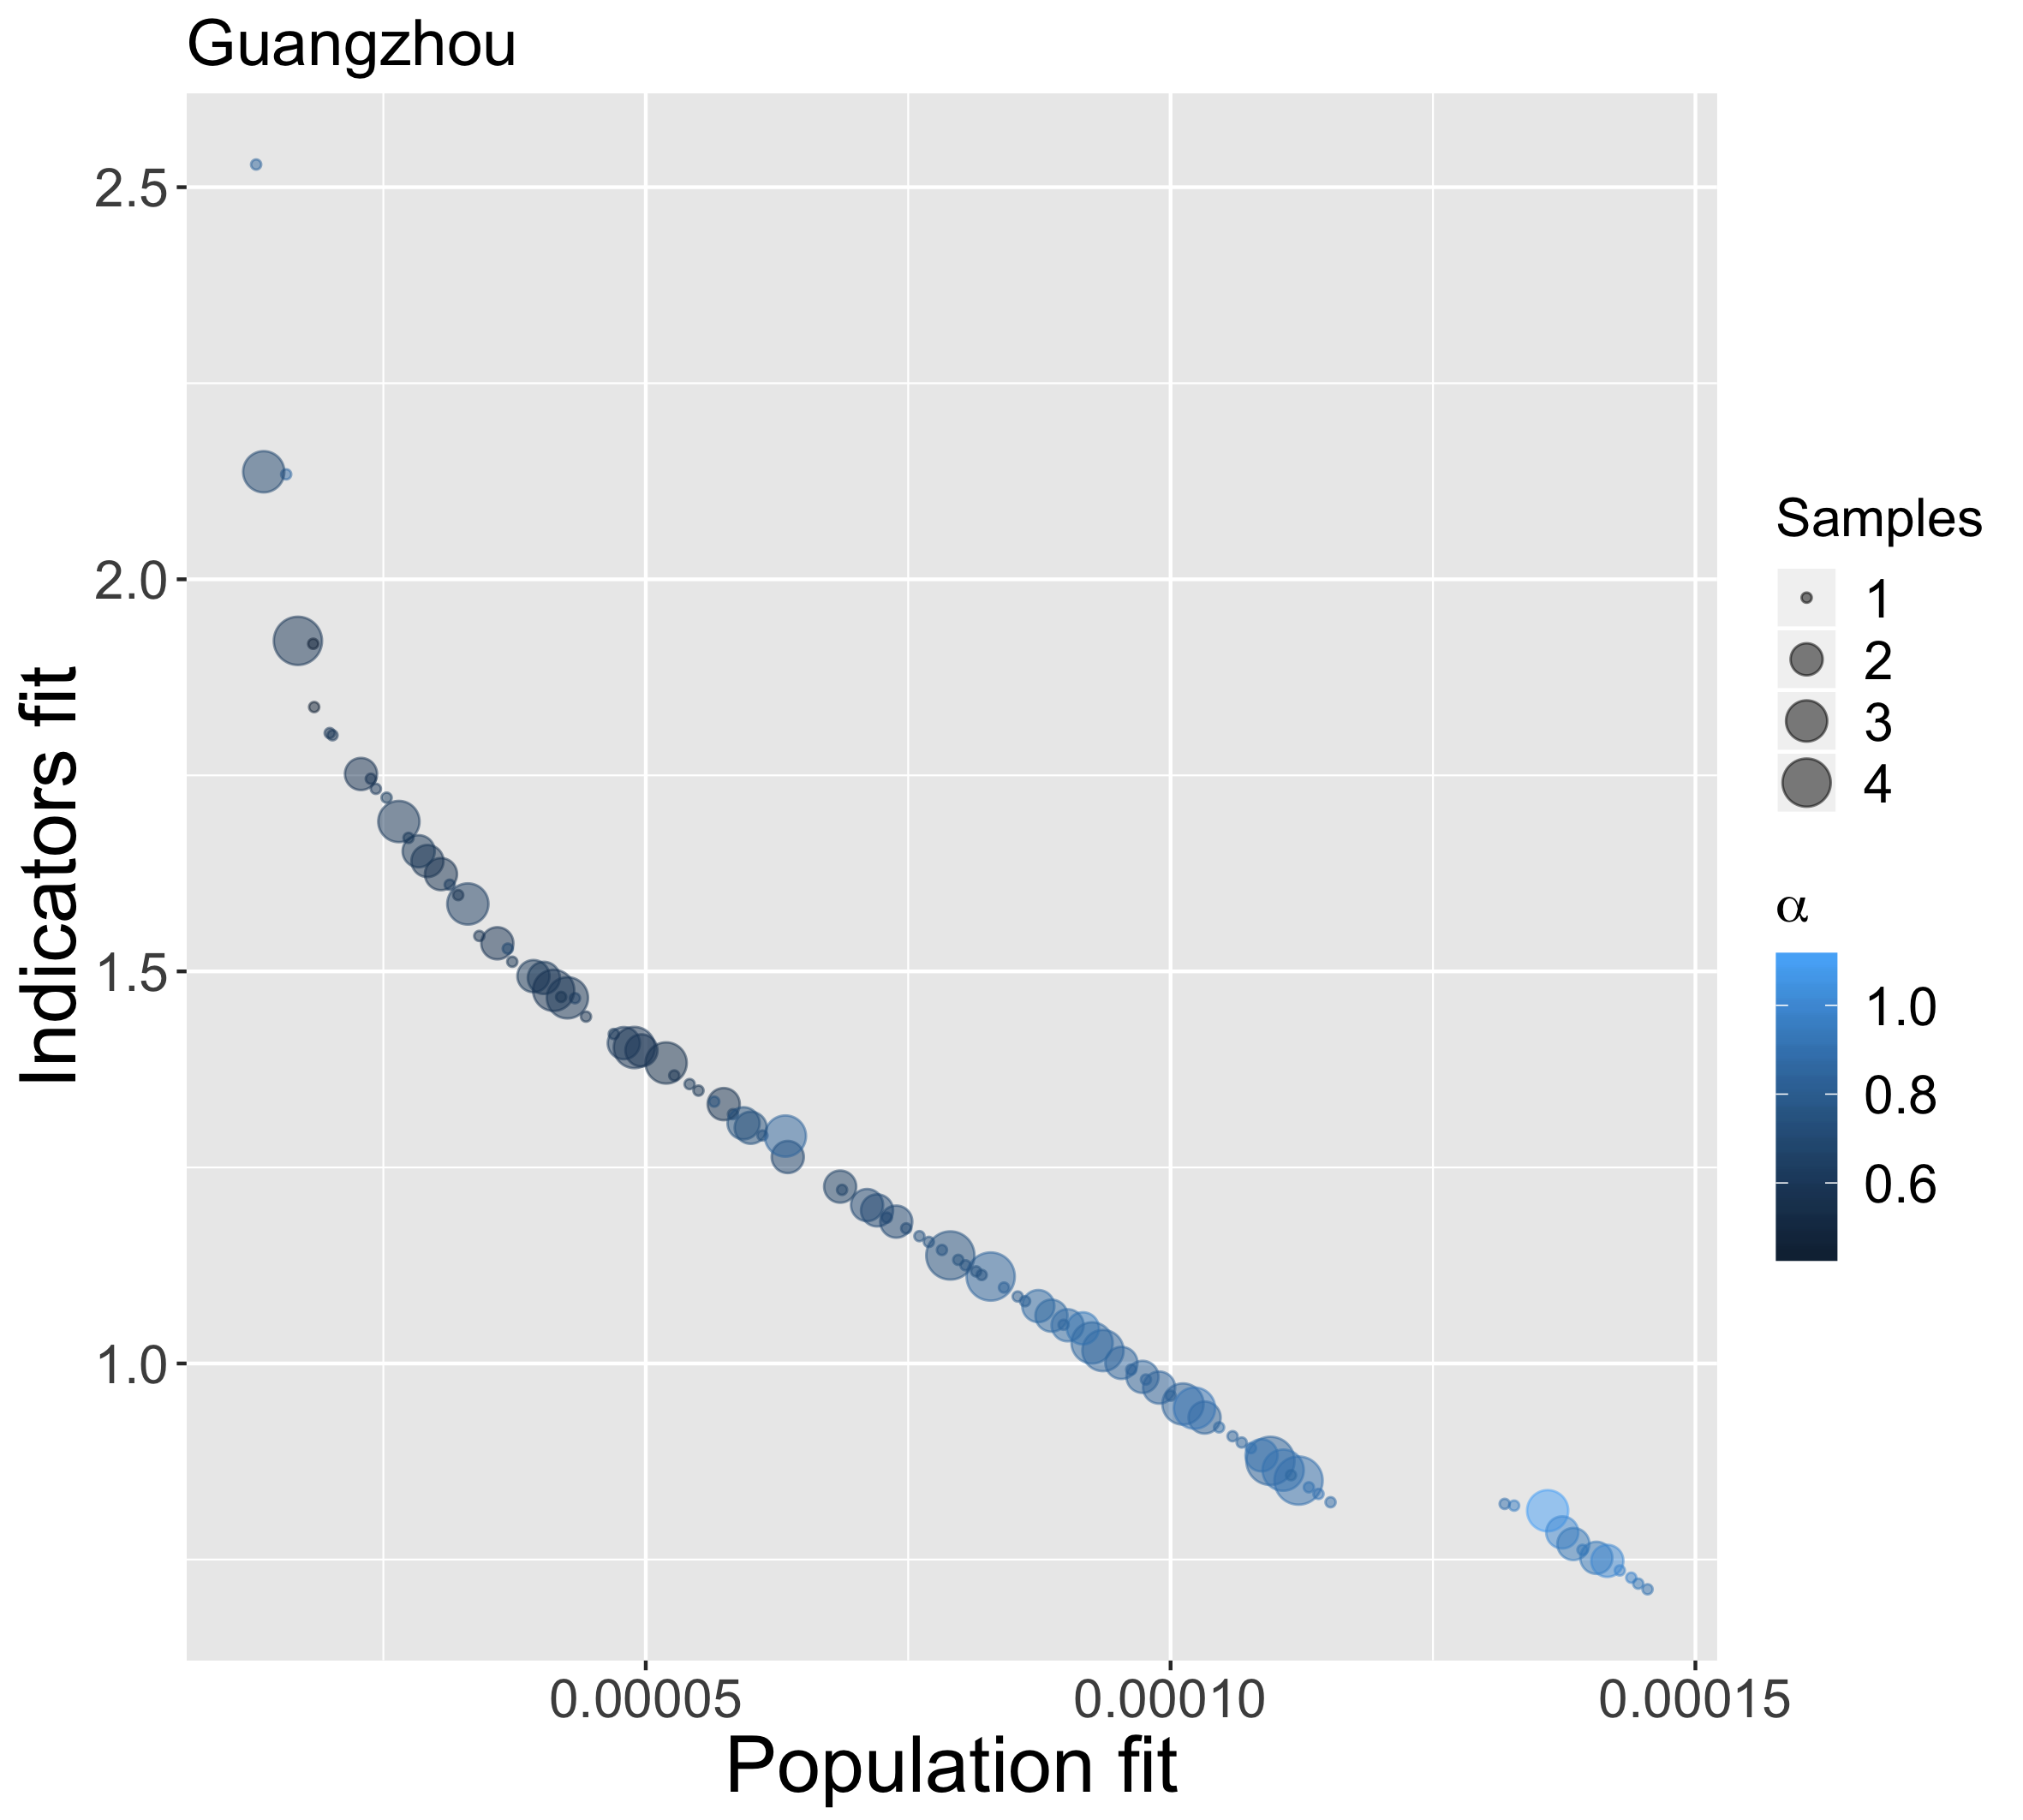
\includegraphics[width=0.49\textwidth]{figures/pareto_indics-relpop_1_coloralpha.png}
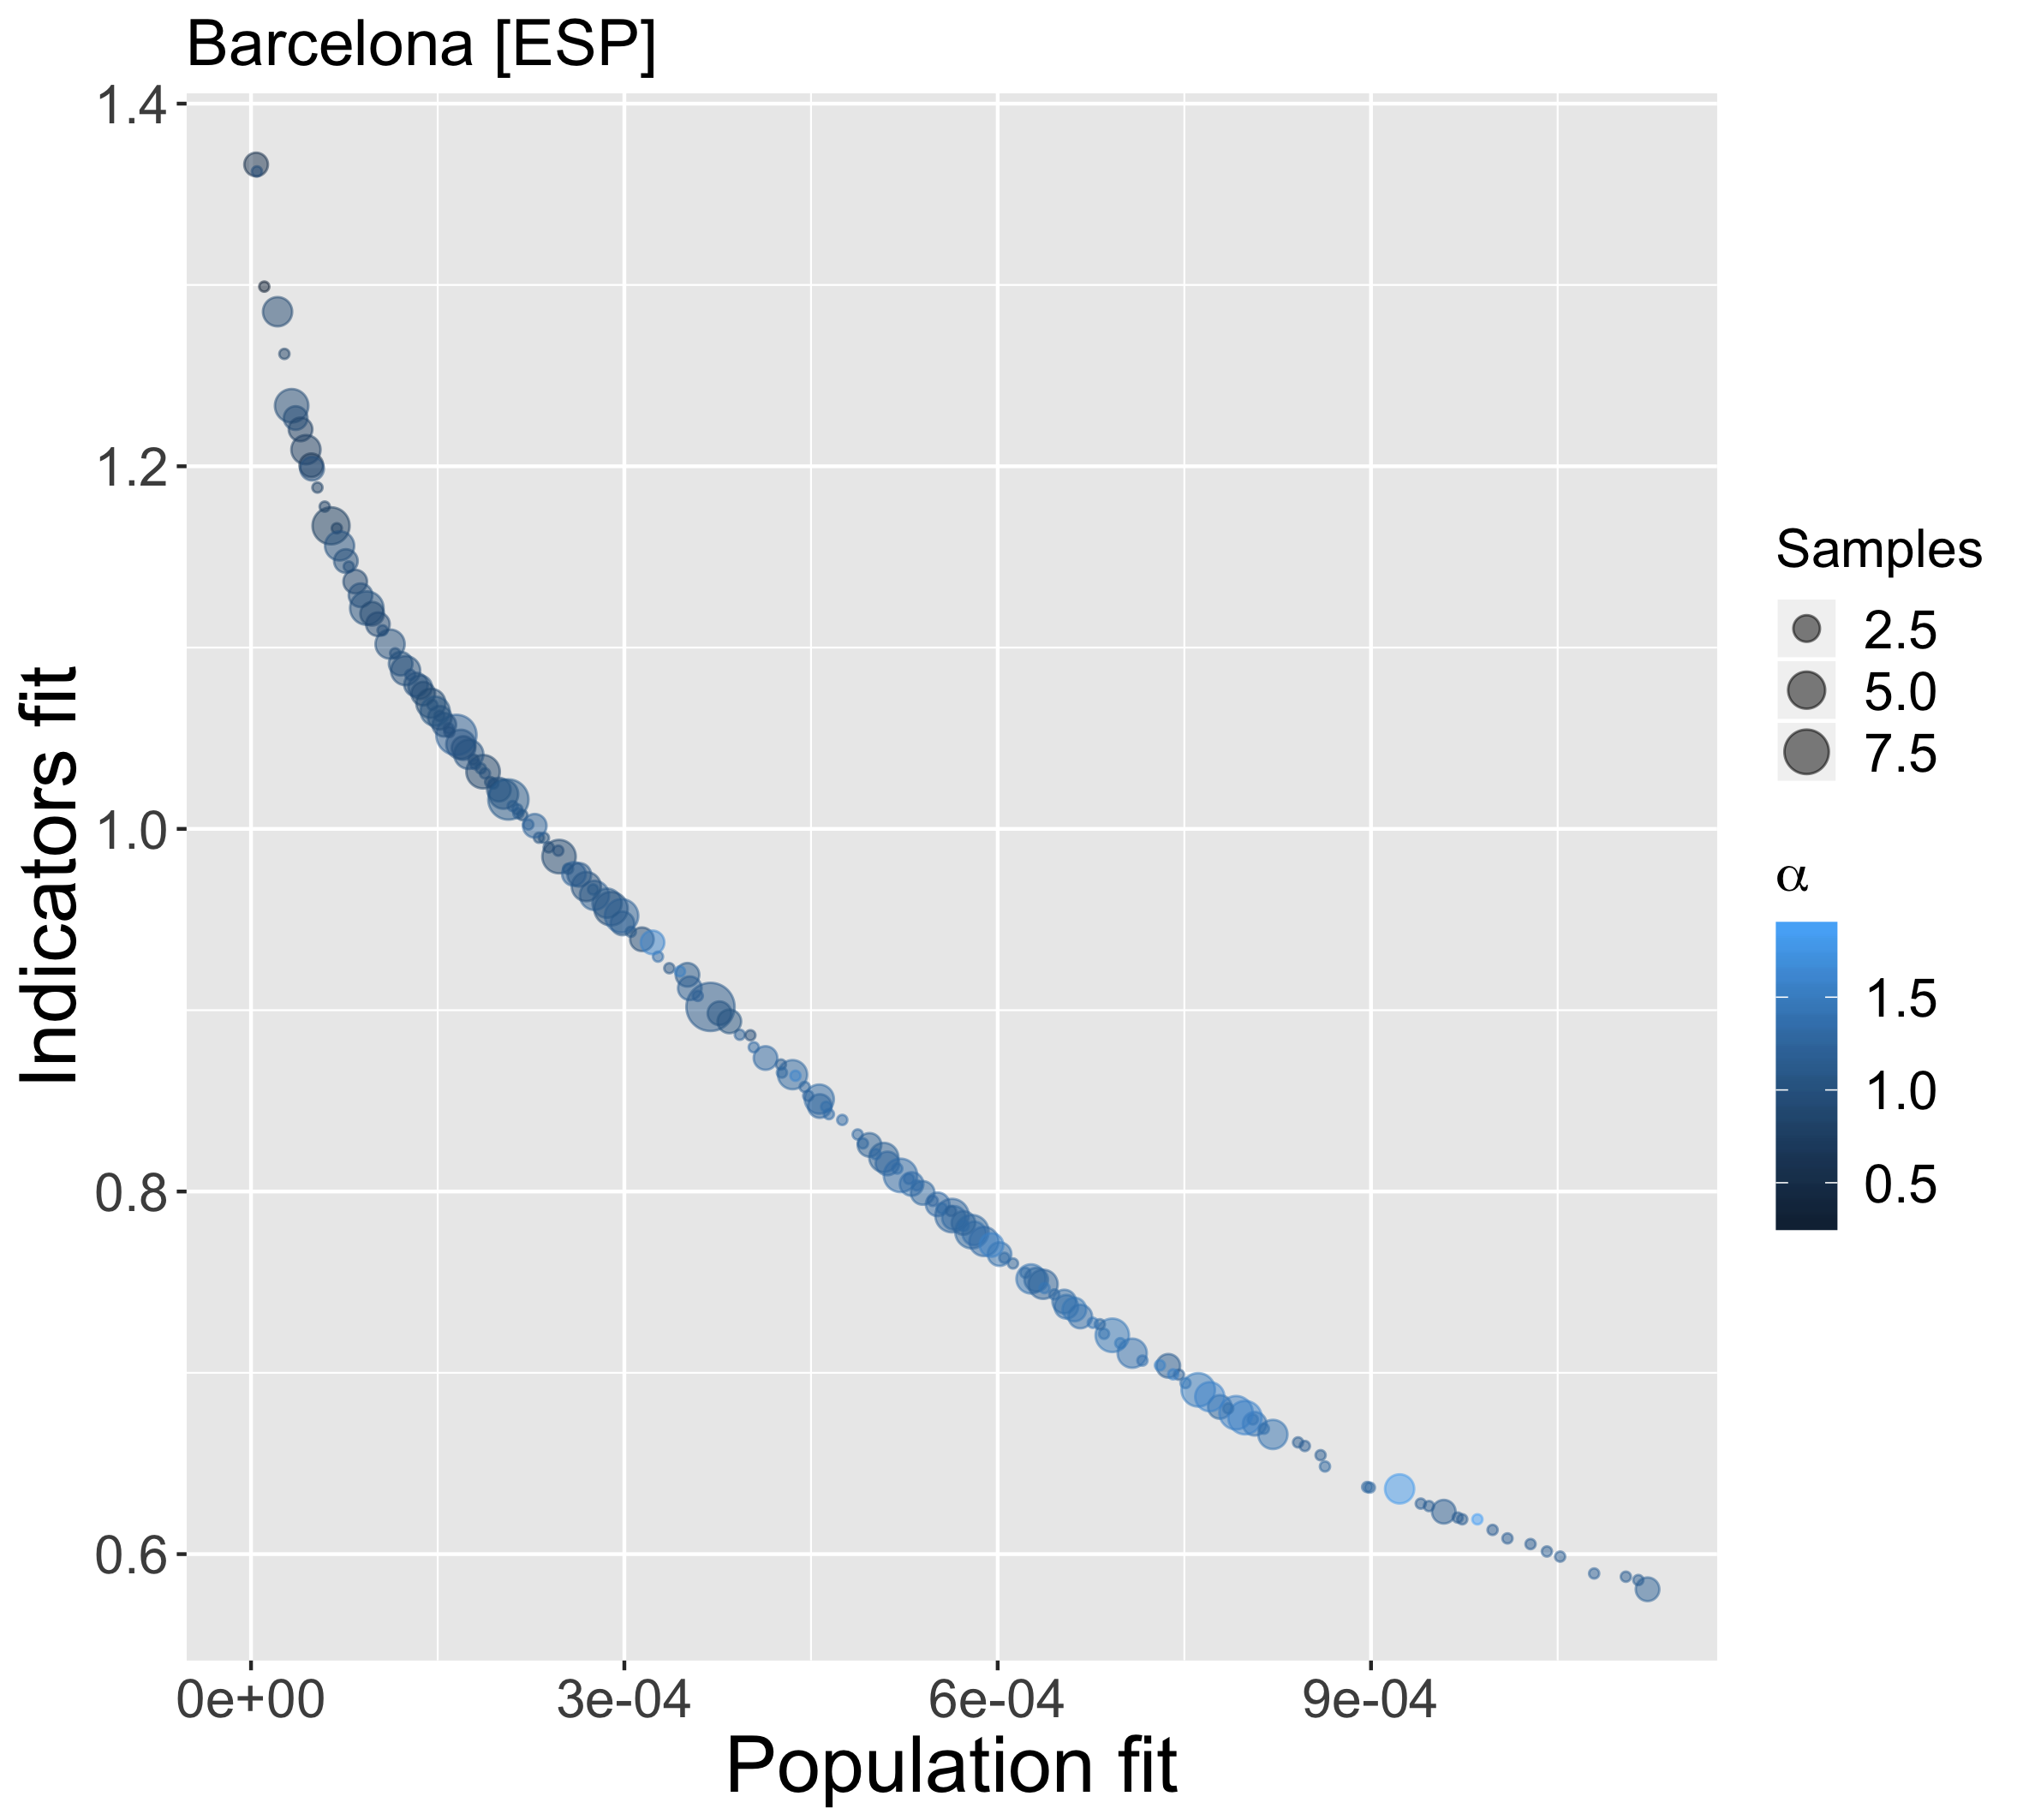
\includegraphics[width=0.49\textwidth]{figures/pareto_indics-relpop_100_coloralpha.png}

\end{center}

\textit{Different performance on indicator fit and forms of Pareto fronts}

}


\sframe{Adjusted parameters}{

% maps : alpha, beta, tstep

% We obtain therein comparable values for aggregation, diffusion and growth speed parameters on all these areas for the three periods given above. 
 
 \centering
 
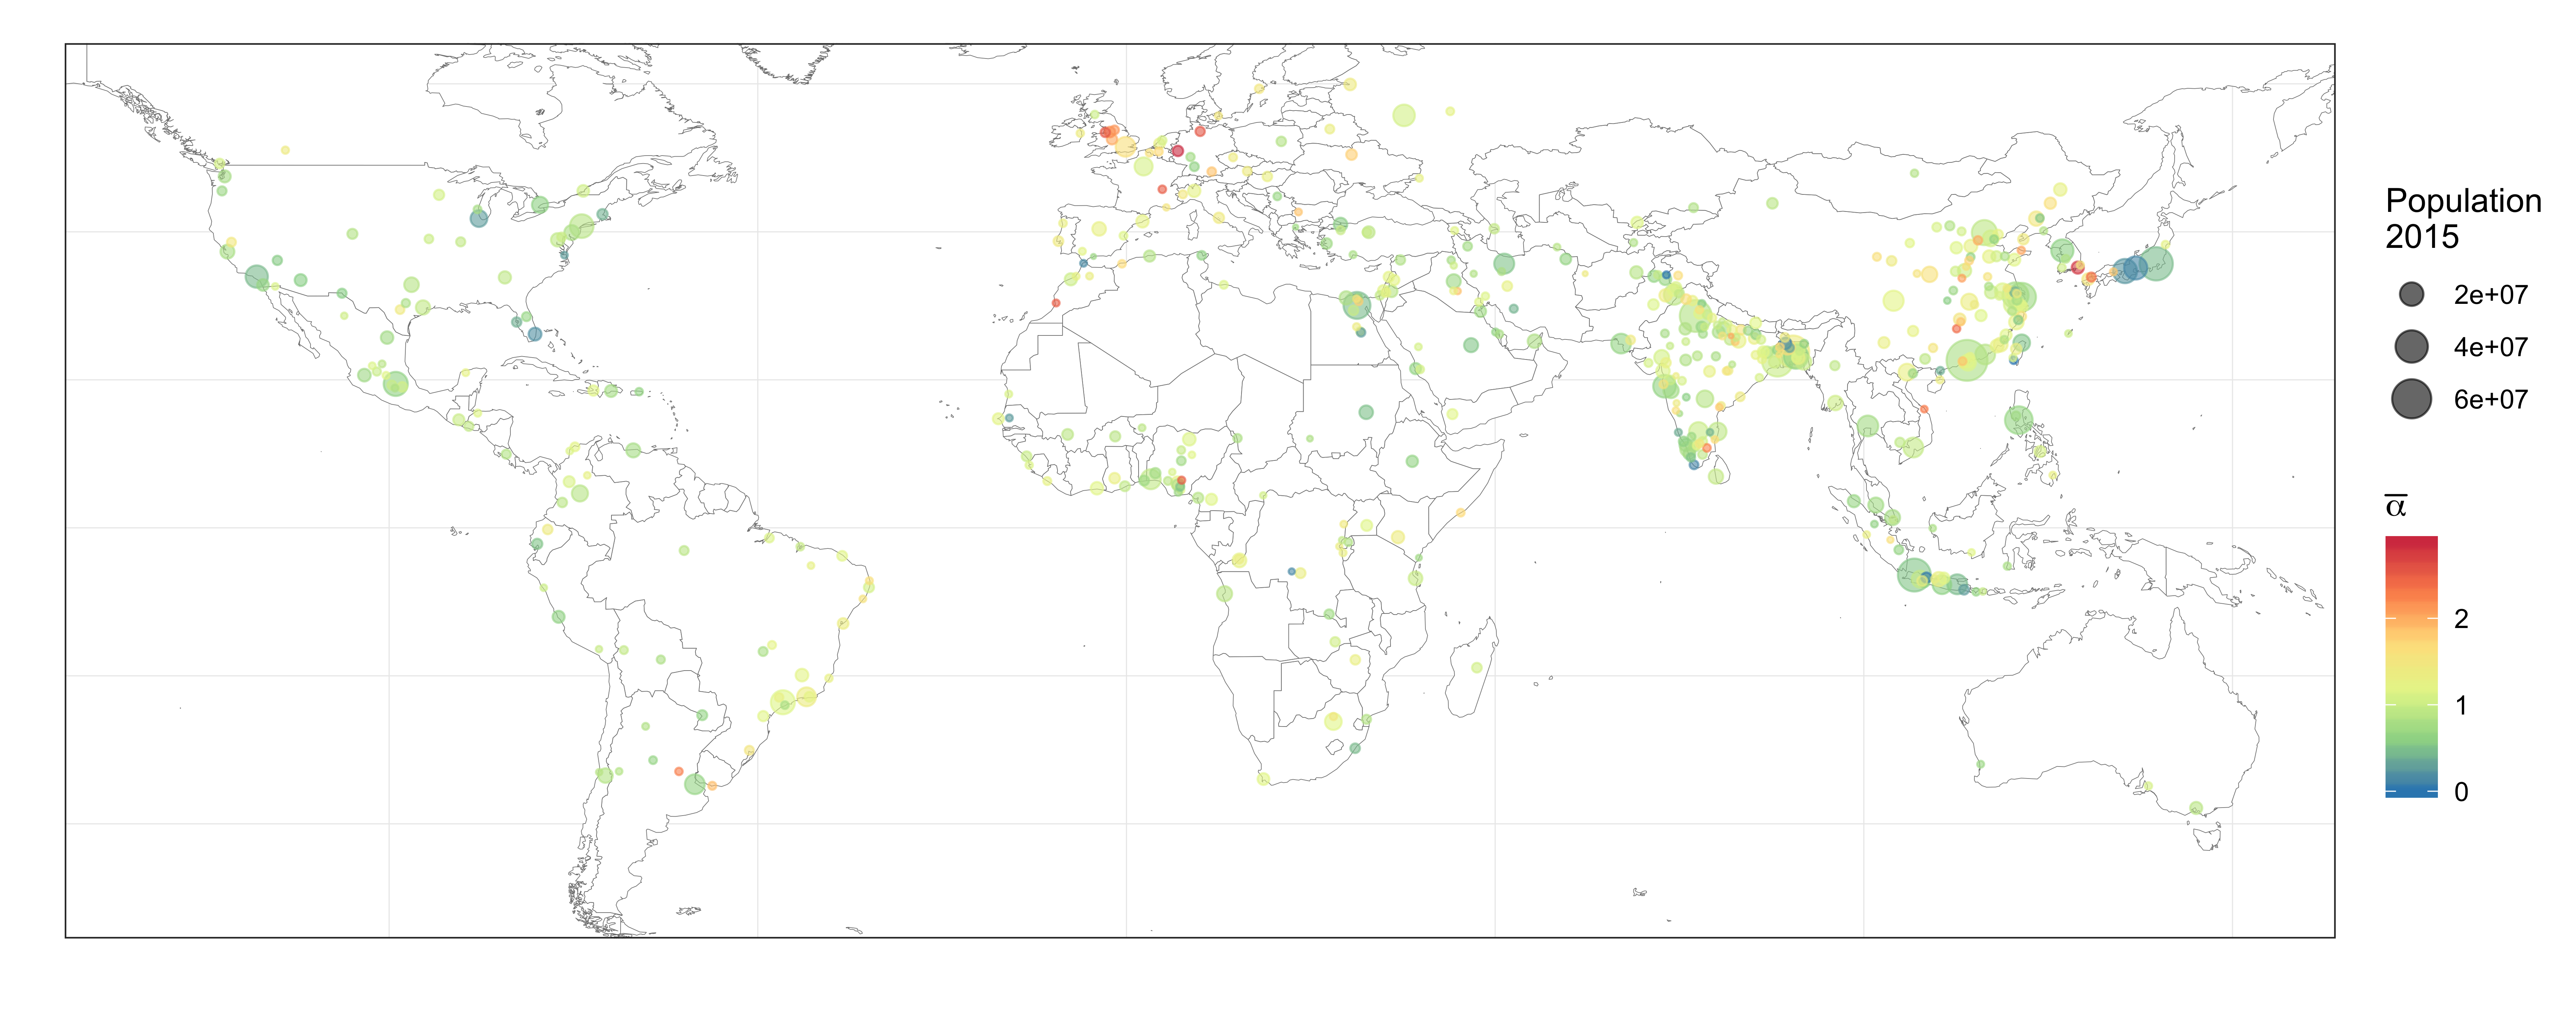
\includegraphics[height=0.43\textheight]{figures/mapparam_meanalpha_2015.png}

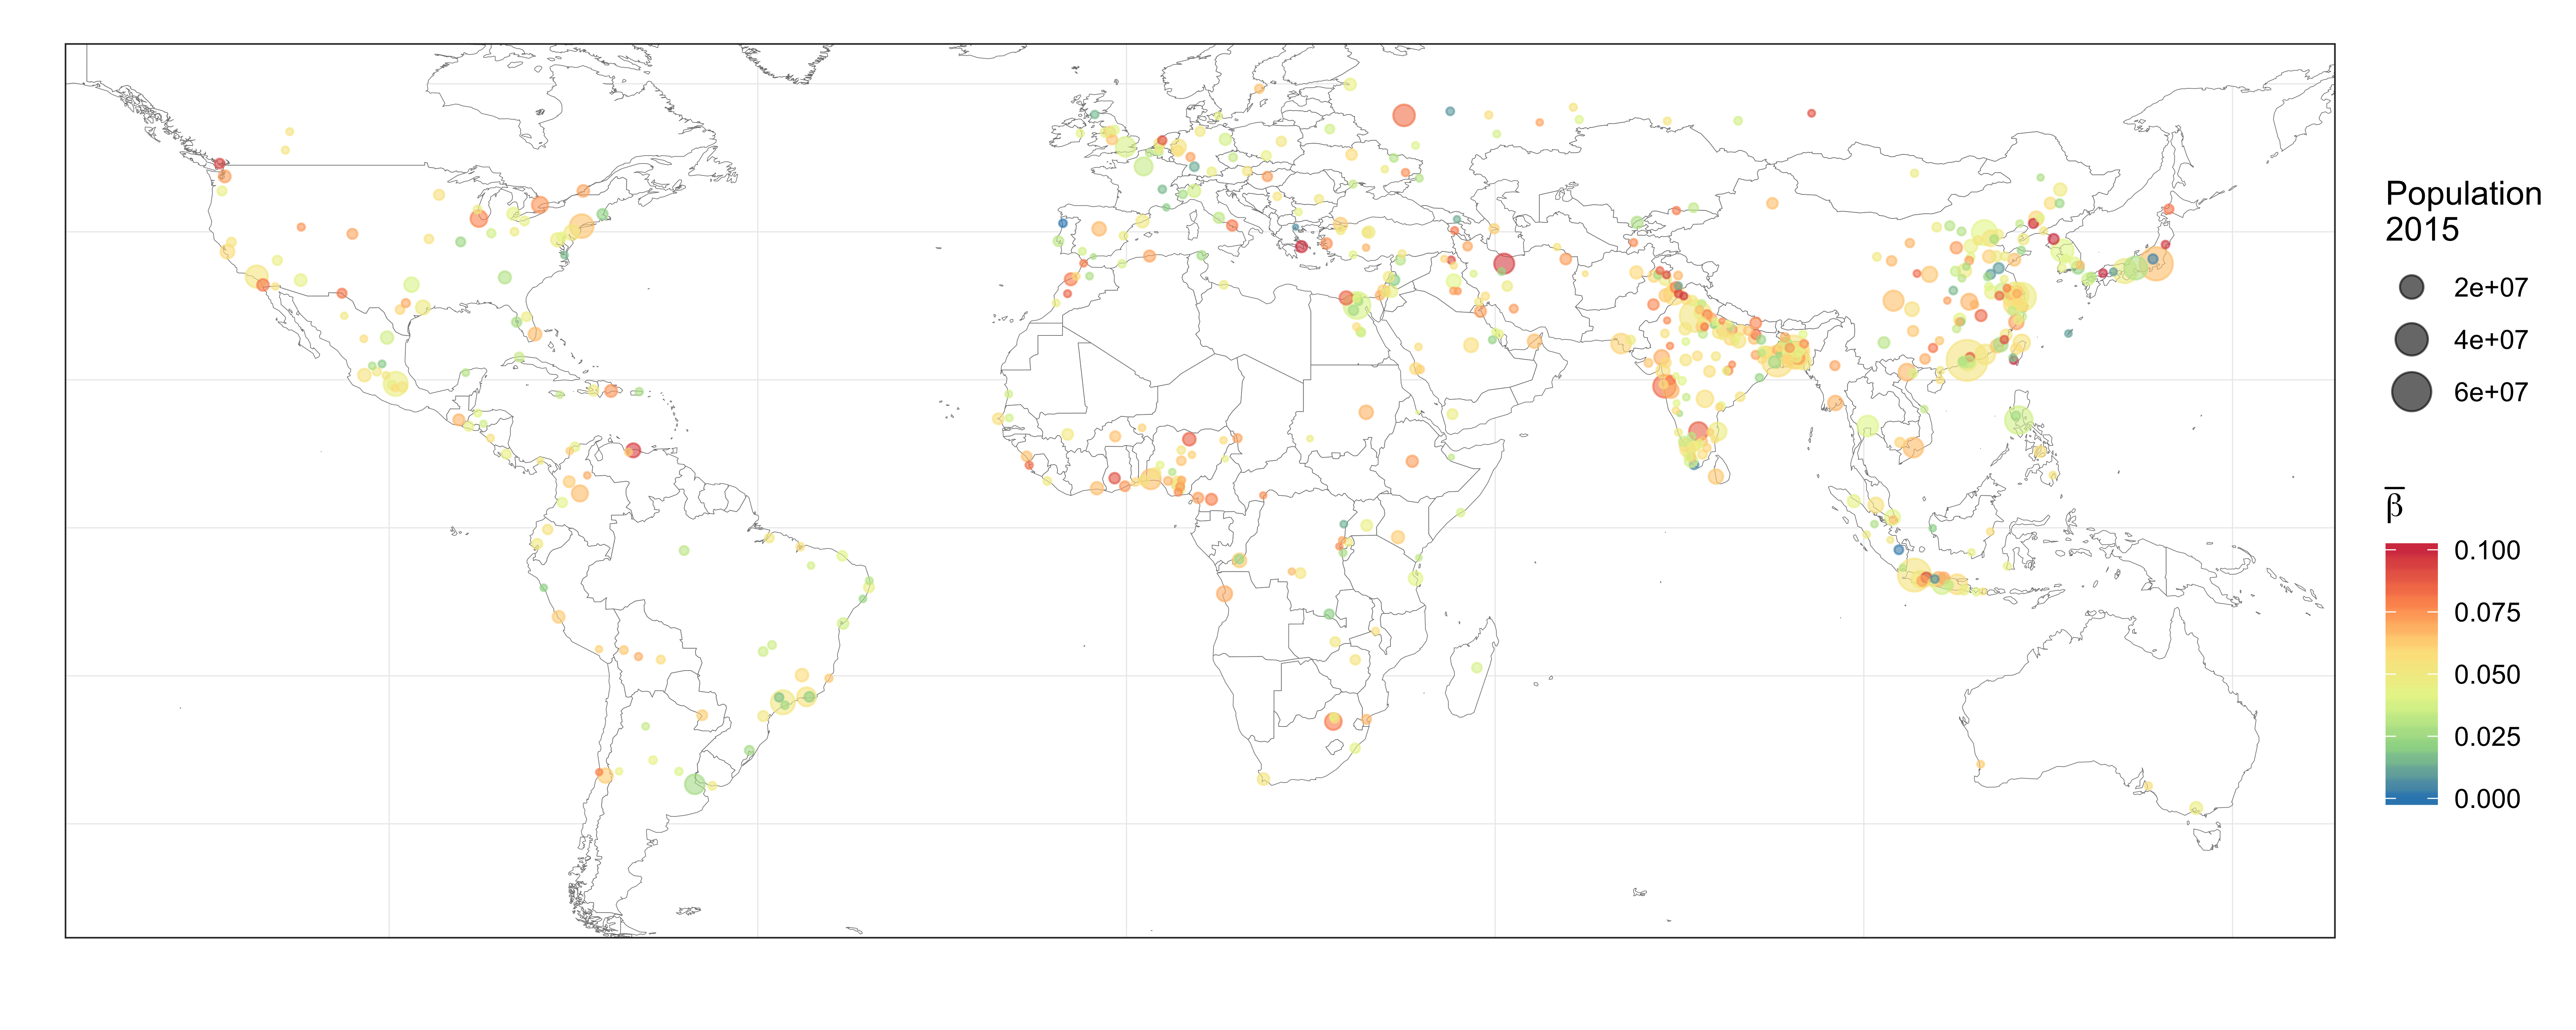
\includegraphics[height=0.43\textheight]{figures/mapparam_meanbeta_2015.png}

 
}


\sframe{Trajectories in phase diagrams}{

% These values can be used for short terms projections, but also high-level policies by situating urban areas in the model phase diagrams and for example comparing them to more or less close phase transition parameter values.

\begin{center}

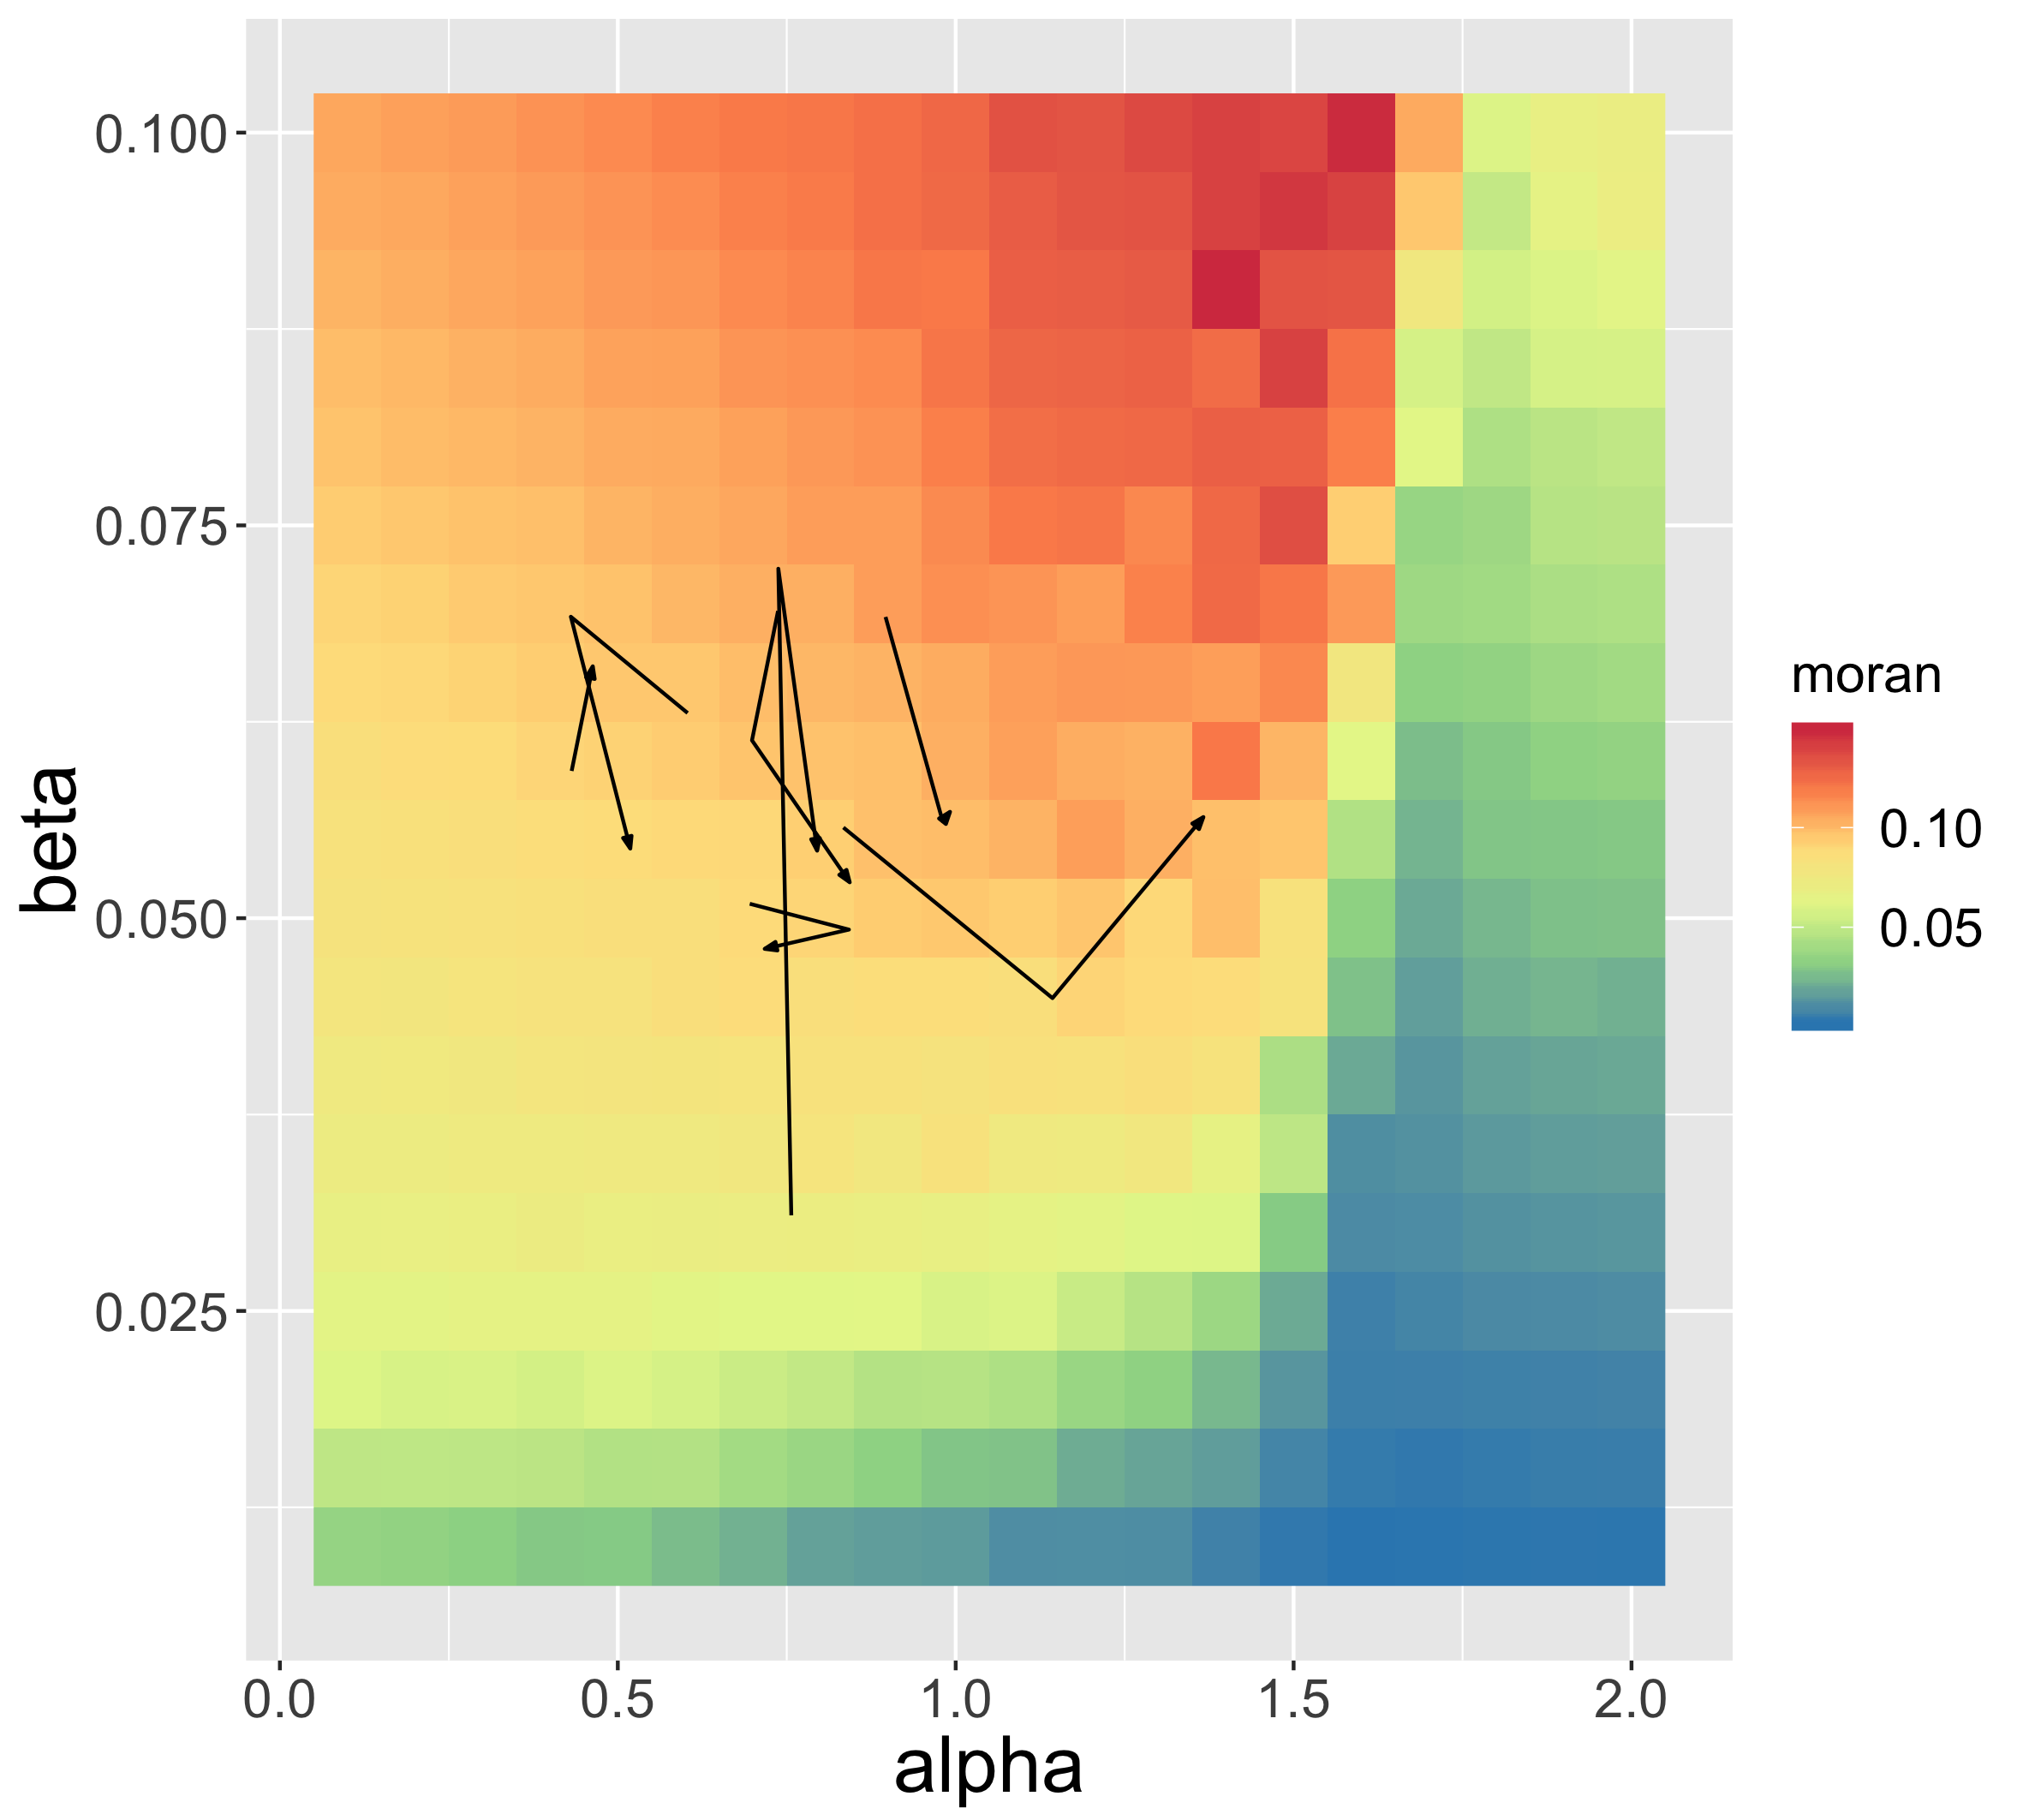
\includegraphics[height=0.49\textheight]{figures/phasediag_largestcities_moran_tsteps50.png}
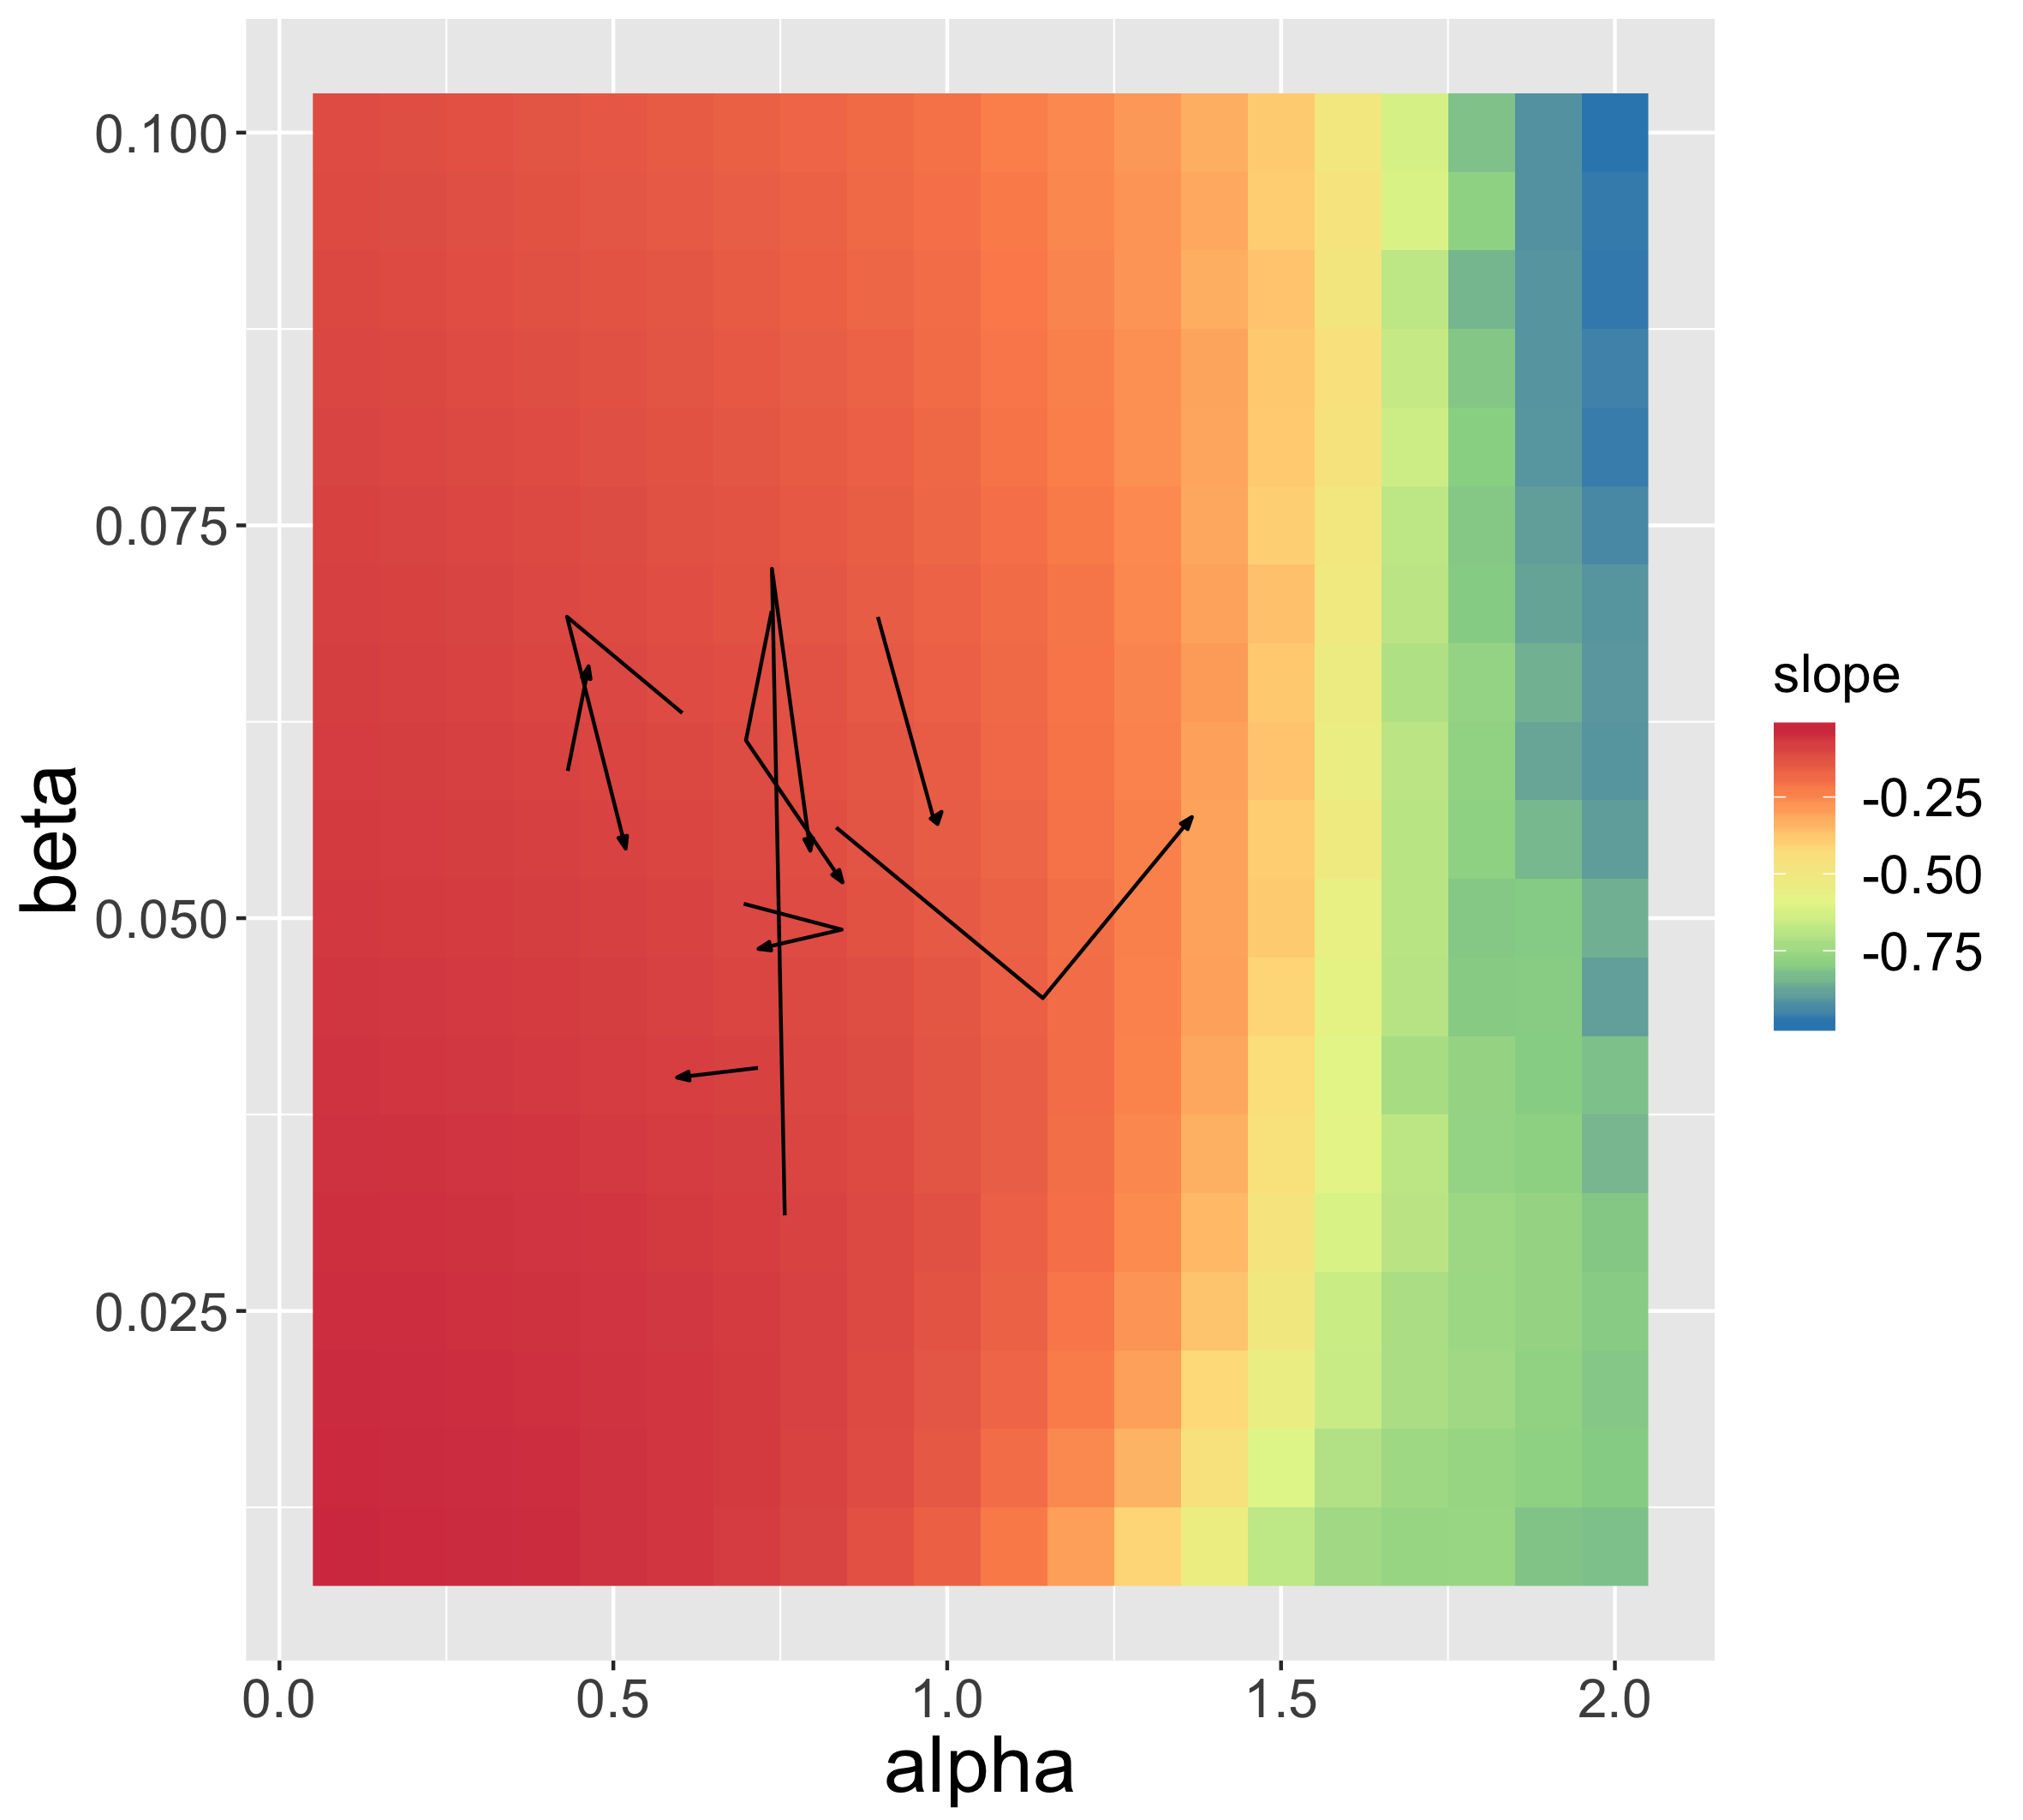
\includegraphics[height=0.49\textheight]{figures/phasediag_largestcities_slope_tsteps50.png}

\end{center}

\textit{Urban areas trajectories can be projected into model phase diagrams}

}


\sframe{Correlations}{

% We also illustrate possible policy applications by relating estimated parameters to the EDGAR greenhouse gases emission database.

\begin{center}

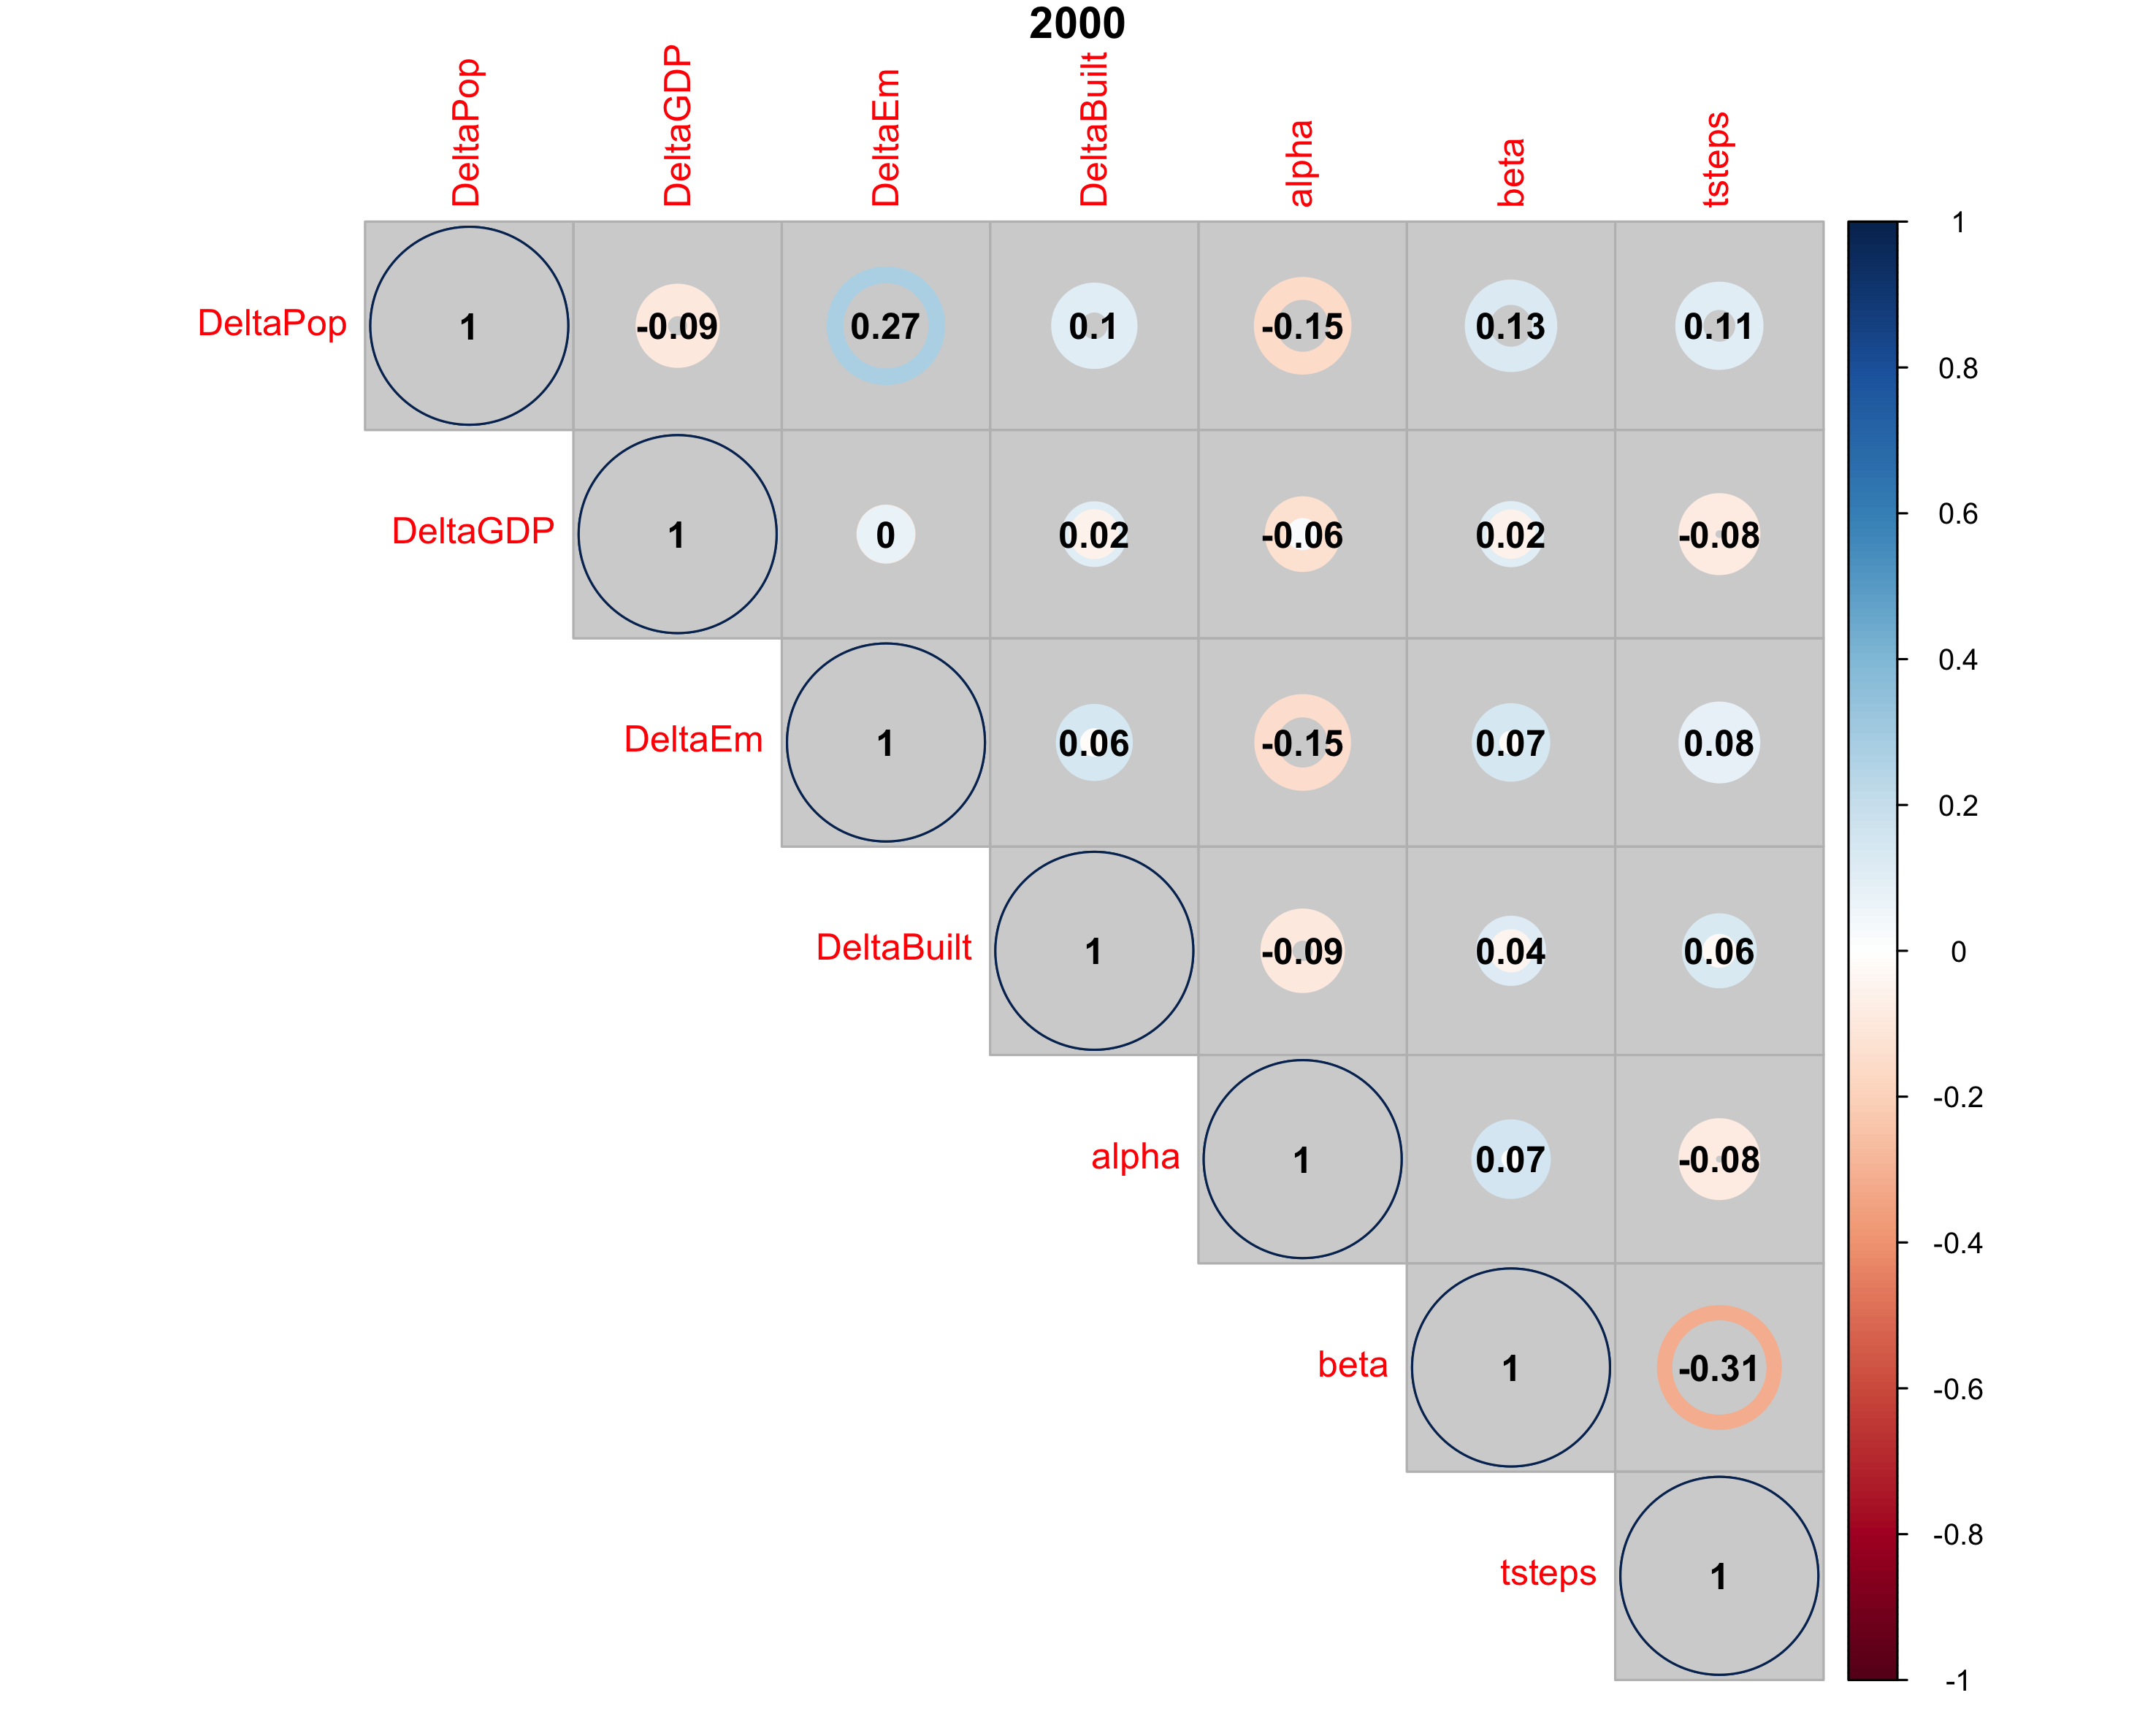
\includegraphics[width=0.49\textwidth]{figures/deltavar-params_2000.png}
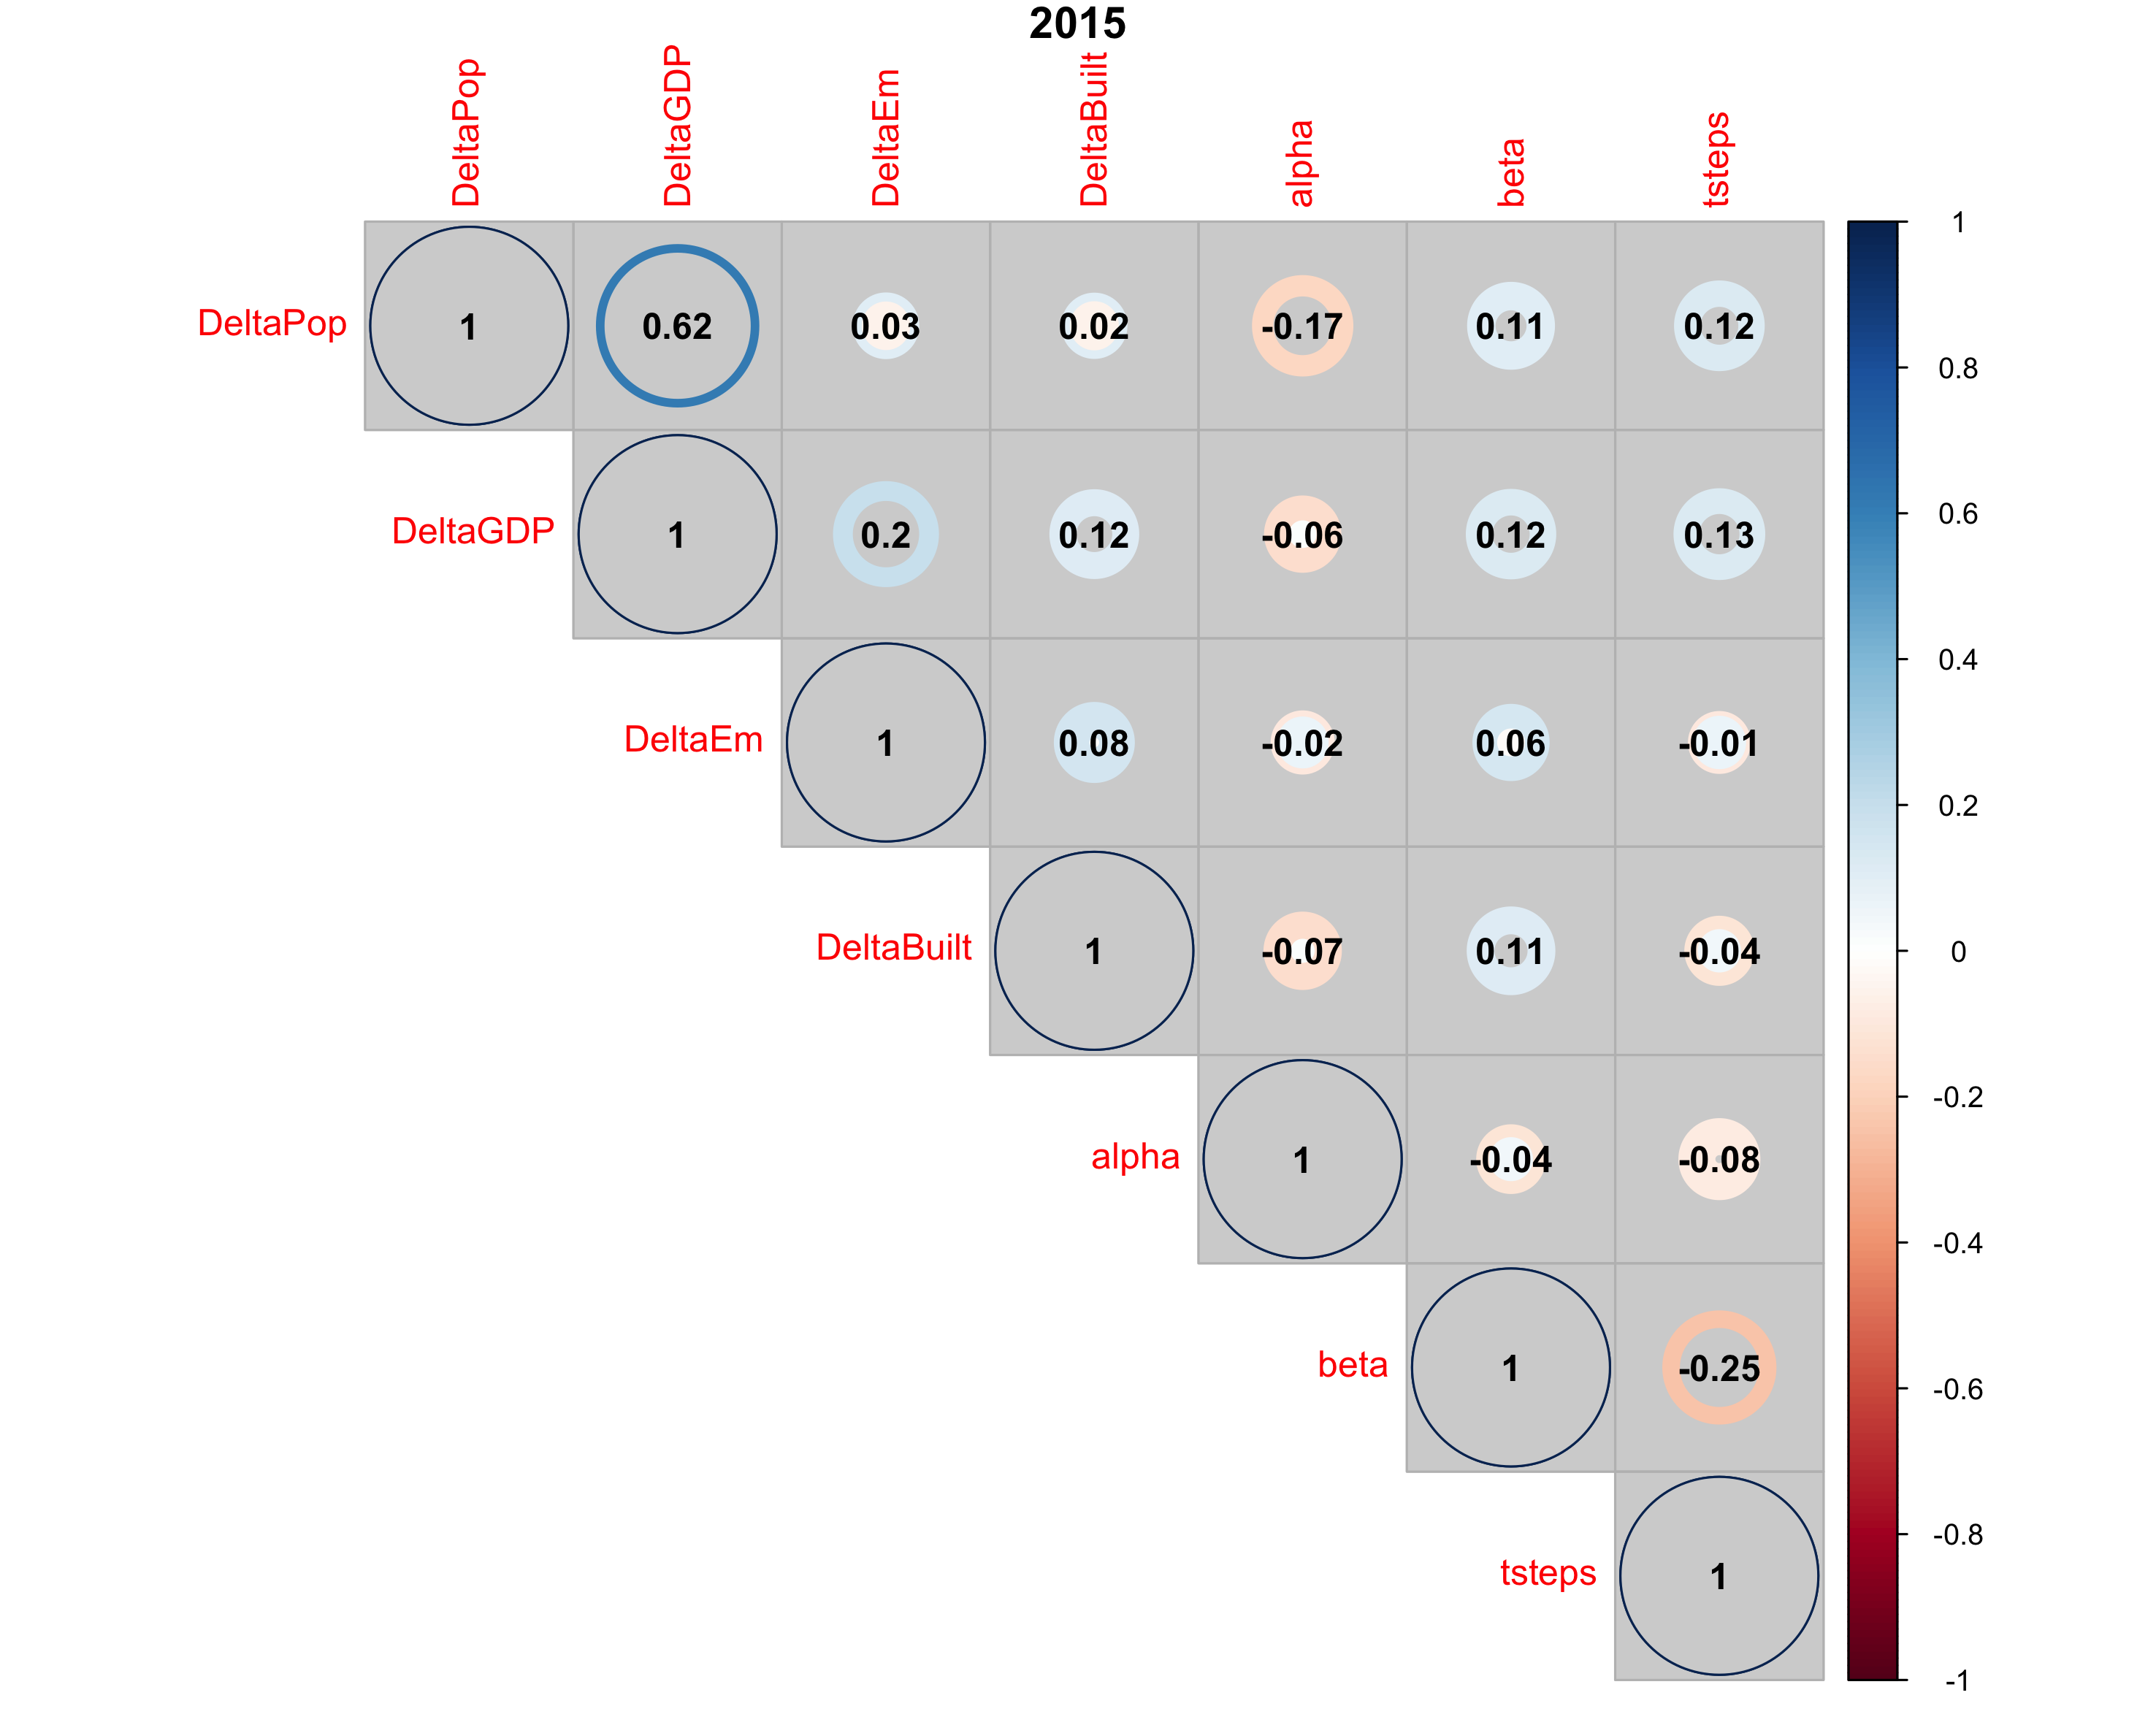
\includegraphics[width=0.49\textwidth]{figures/deltavar-params_2015.png}

\end{center}

\textit{Slight significant correlations with growth rates of GHG emissions: more aggregation correlates with decreasing emissions e.g.}


}




\section{Discussion}



\sframe{Discussion}{

%  This work thus shows how simple models can be useful for global comparisons, which are necessary to contextualize territorial policies.


% \textit{Which ontology to include more complex functional properties ?}
%$\rightarrow$ Territorial systems as the strong coupling between territories and (potential and realized) networks \cite{dupuy1987vers}.
%$\rightarrow$ Networks convey functional notions of centralities and accessibility, among others; have furthermore proper topological properties.



\justify

\vspace{-1cm}

\textbf{Implications}

\smallskip

$\rightarrow$ This rather simple model can effectively be calibrated on worldwide urban areas and provide comparable growth parameters

\medskip

$\rightarrow$ Link between urban form, urban dynamics and sustainability properties


\bigskip

\textbf{Developments}

\smallskip

$\rightarrow$ Benchmark with other simple models (e.g. \cite{li2019singularity} presented yesterday)

\medskip

$\rightarrow$ Coupling with macro-scale model for system of cities \cite{raimbault:halshs-02351722}


\medskip

$\rightarrow$ Investigate the link between spatial non-stationarity and non-ergodicity through simulation by the model

%$\rightarrow$ Compare network generation in a ``fair'' way (correcting for additional parameters, open question for models of simulation)


}



\sframe{Towards policy applications}{

% more data

\justify

Within the same stream of modeling (complementary to more classical approaches to land-use change):

\medskip

\textbf{More realistic models?}

\smallskip

$\rightarrow$ Introducing more concrete ontologies, economic processes \\
\cite{bonin2014modelisation}, qualitative differentiation \cite{bonin2012modele}, governance processes \cite{le2015modeling}

\medskip

$\rightarrow$ Possible bridges with Land-use change models/Land-use Transport models \cite{wegener2004land}, with systems of cities models\\
 \cite{pumain2017urban}

\medskip

\textbf{More data-driven models?}

\smallskip


$\rightarrow$ More systematic link with sustainability indicators: GHG emissions, economics, etc. \cite{raimbault2019multi}

\medskip

$\rightarrow$ Study models on hybrid synthetic data \cite{raimbault2018space}: systematic conclusions for policies



}




\sframe{Conclusion}{


\justify

$\rightarrow$ A simple model of urban morphogenesis at the mesoscopic scale systematically calibrated: \textbf{need for more benchmarking and comparison of models.}

\smallskip

$\rightarrow$ At the macro scale of the system of cities? \textbf{Need for multi-scale models.}

\smallskip

$\rightarrow$ With more refined urban characteristics and other dimensions ? \textbf{Need for more interdisciplinarity.}

\bigskip
\bigskip

\textbf{Use and contribute to OpenMOLE: } \url{https://github.com/openmole}

\bigskip

\textbf{Apply to the summer school: } \url{https://exmodelo.org/}


\bigskip
\bigskip

\footnotesize{ - Code, data and results available at \texttt{https://github.com/JusteRaimbault/UrbanGrowth}\\
- Acknowledgments: Thanks to the \textit{European Grid Infrastructure} and its \textit{National Grid Initiatives} (\textit{France-Grilles} in particular) to give the technical support and the infrastructure.

}

}



\section*{Reserve slides}


\sframe{Reserve slides}{

\centering

\Large

\textbf{Reserve Slides}

}



\sframe{Generating Population Distributions}{


% examples : fig 2 of paper

\centering

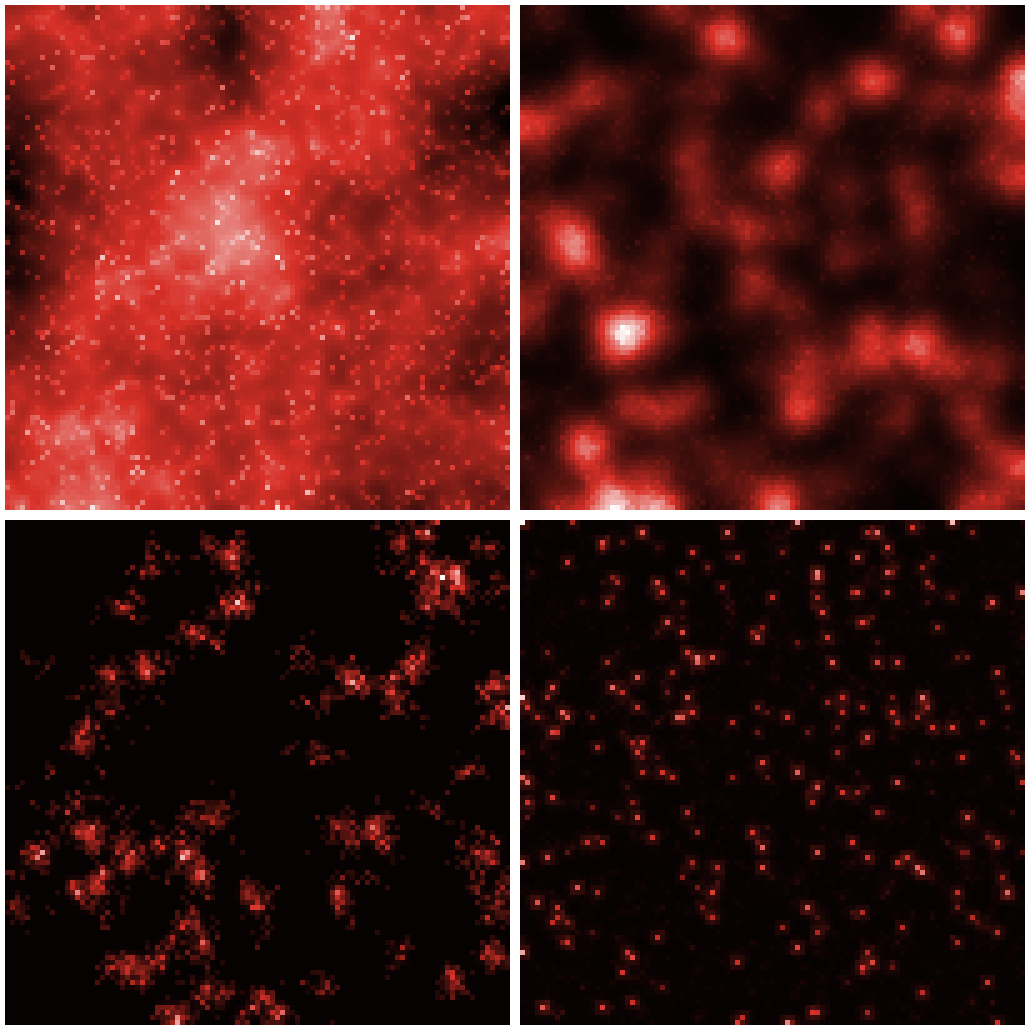
\includegraphics[height=0.8\textheight]{figures/density_Fig2}

\footnotesize\textit{Examples of generated territorial shapes}

}


\sframe{Path-dependence and frozen accidents}{

\centering

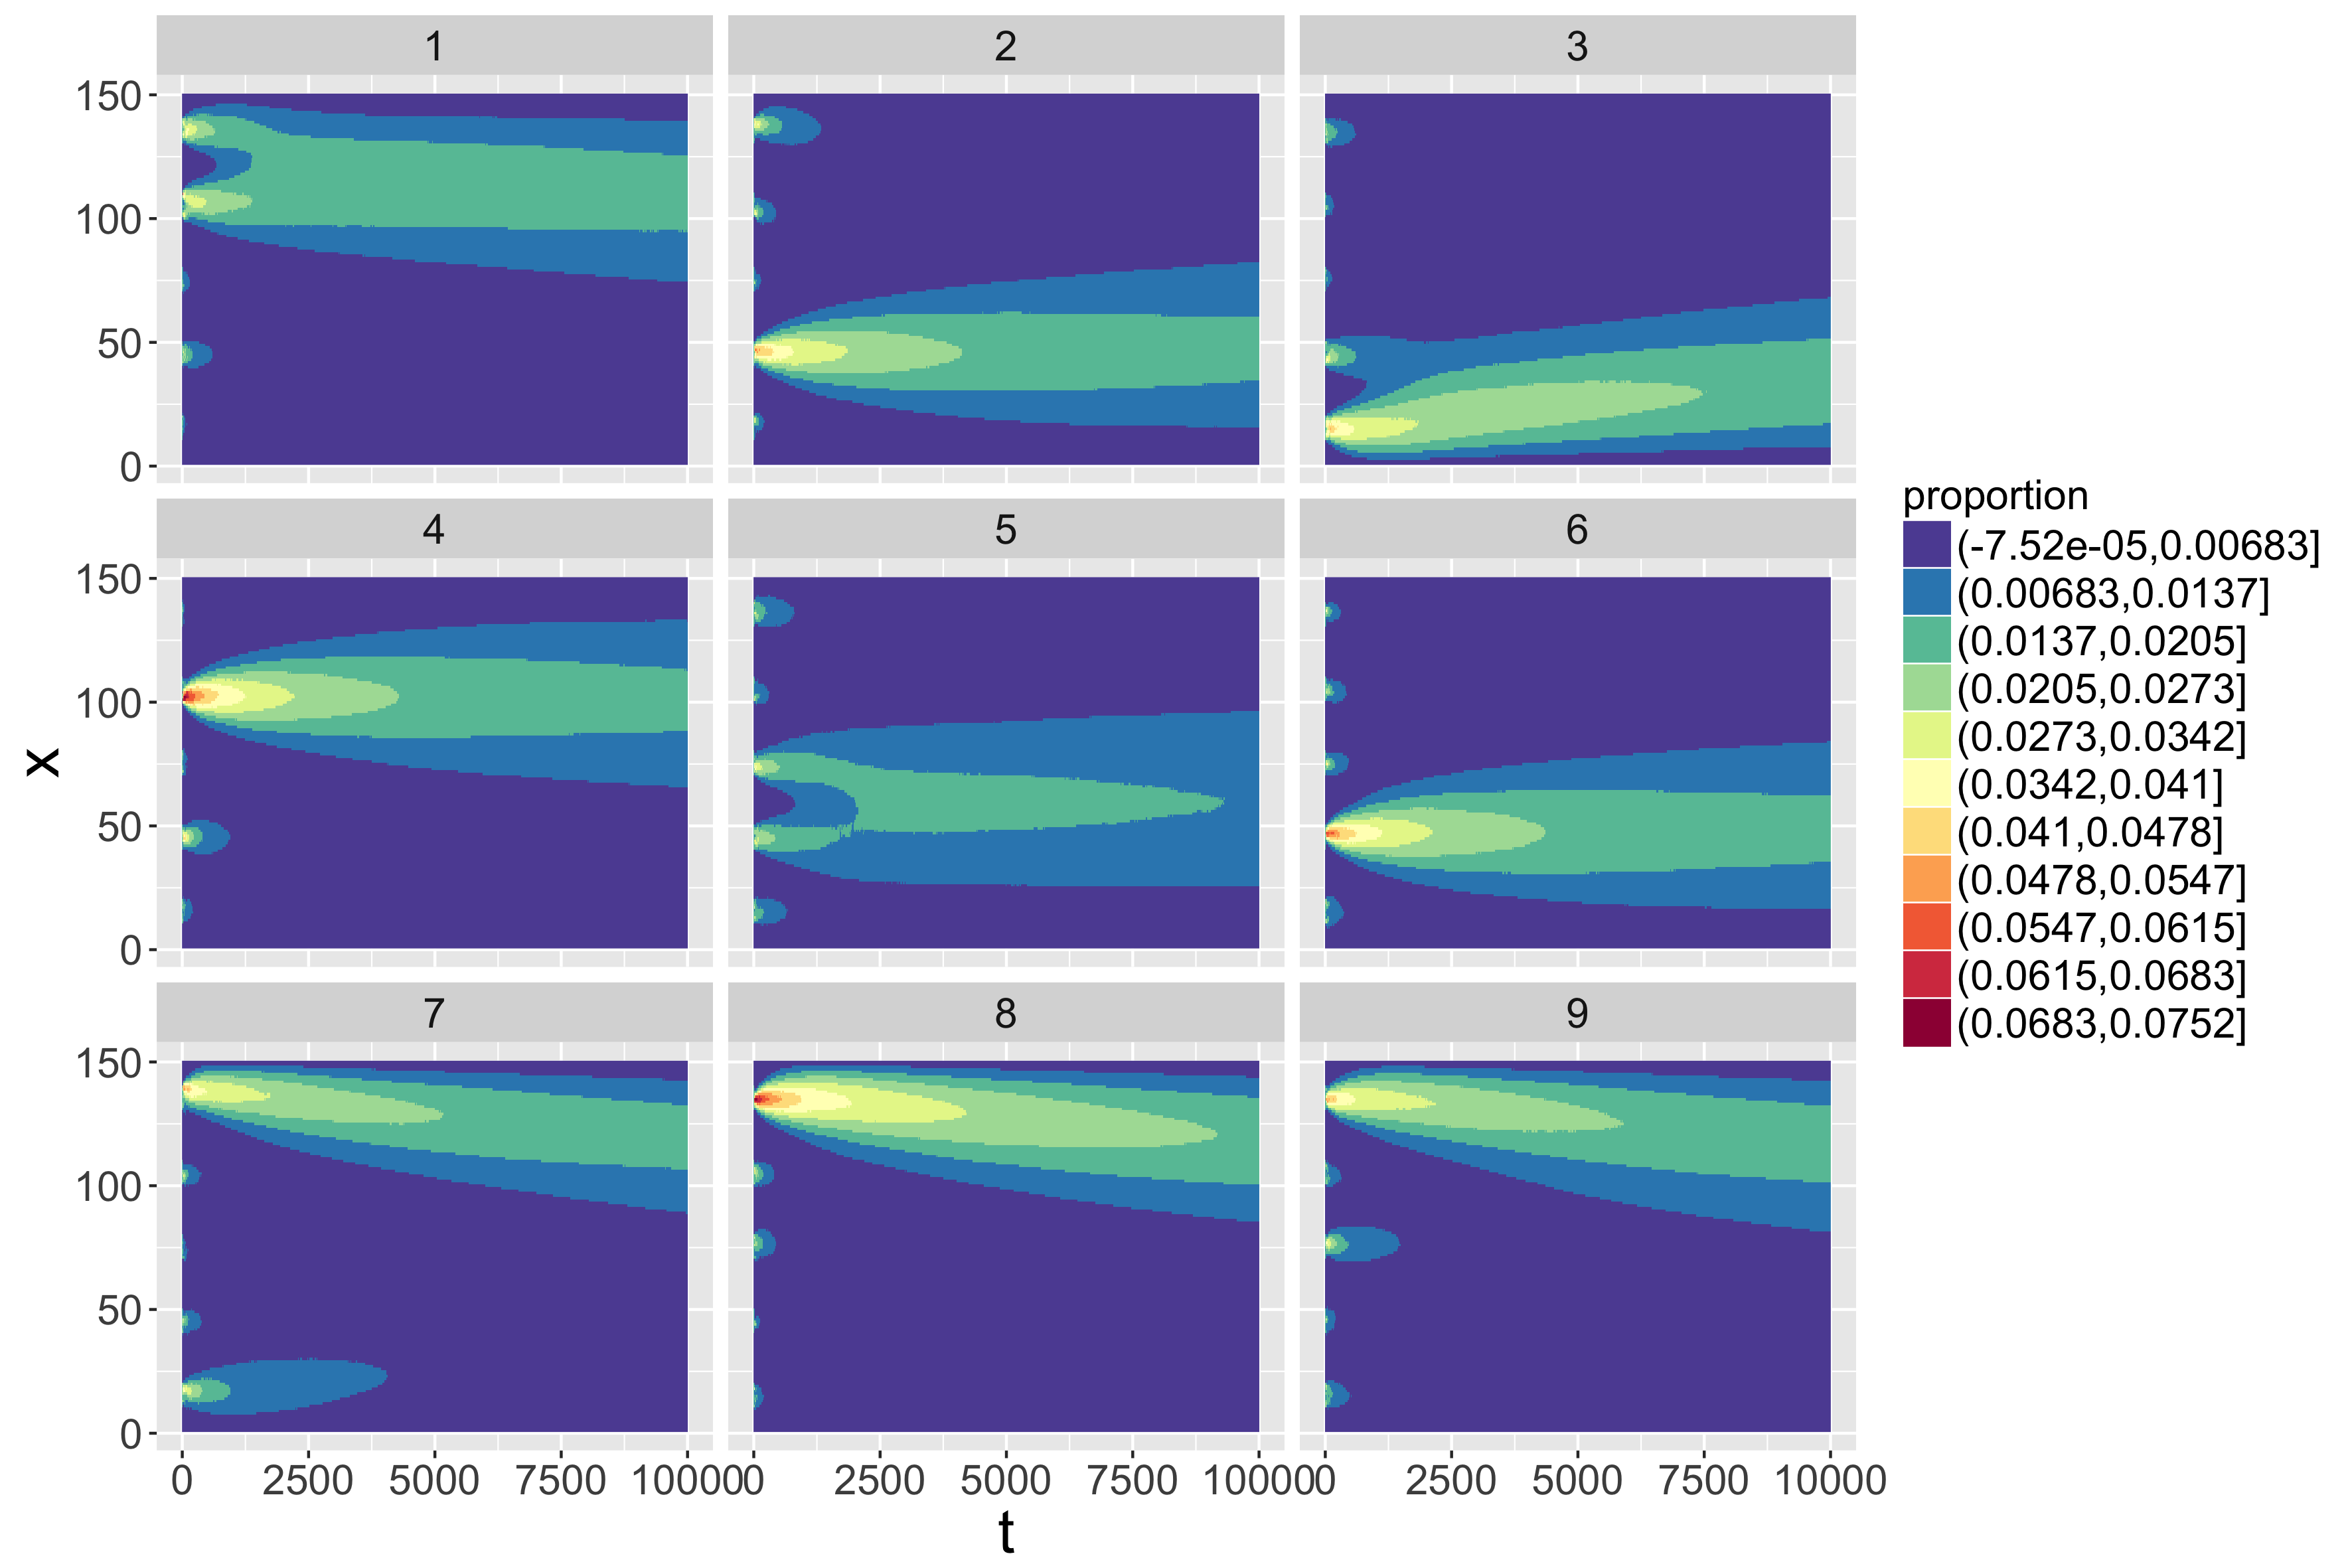
\includegraphics[width=0.8\textwidth]{figures/density_Fig4}

\footnotesize\textit{Illustration of path-dependence in a simplified one-dimensional version of the model: cell trajectories in time for 9 independent repetitions from the same initial configuration.}


}




\sframe{Empirical Data (moving window)}{


\begin{columns}
\column{0.6\textwidth}
\centering
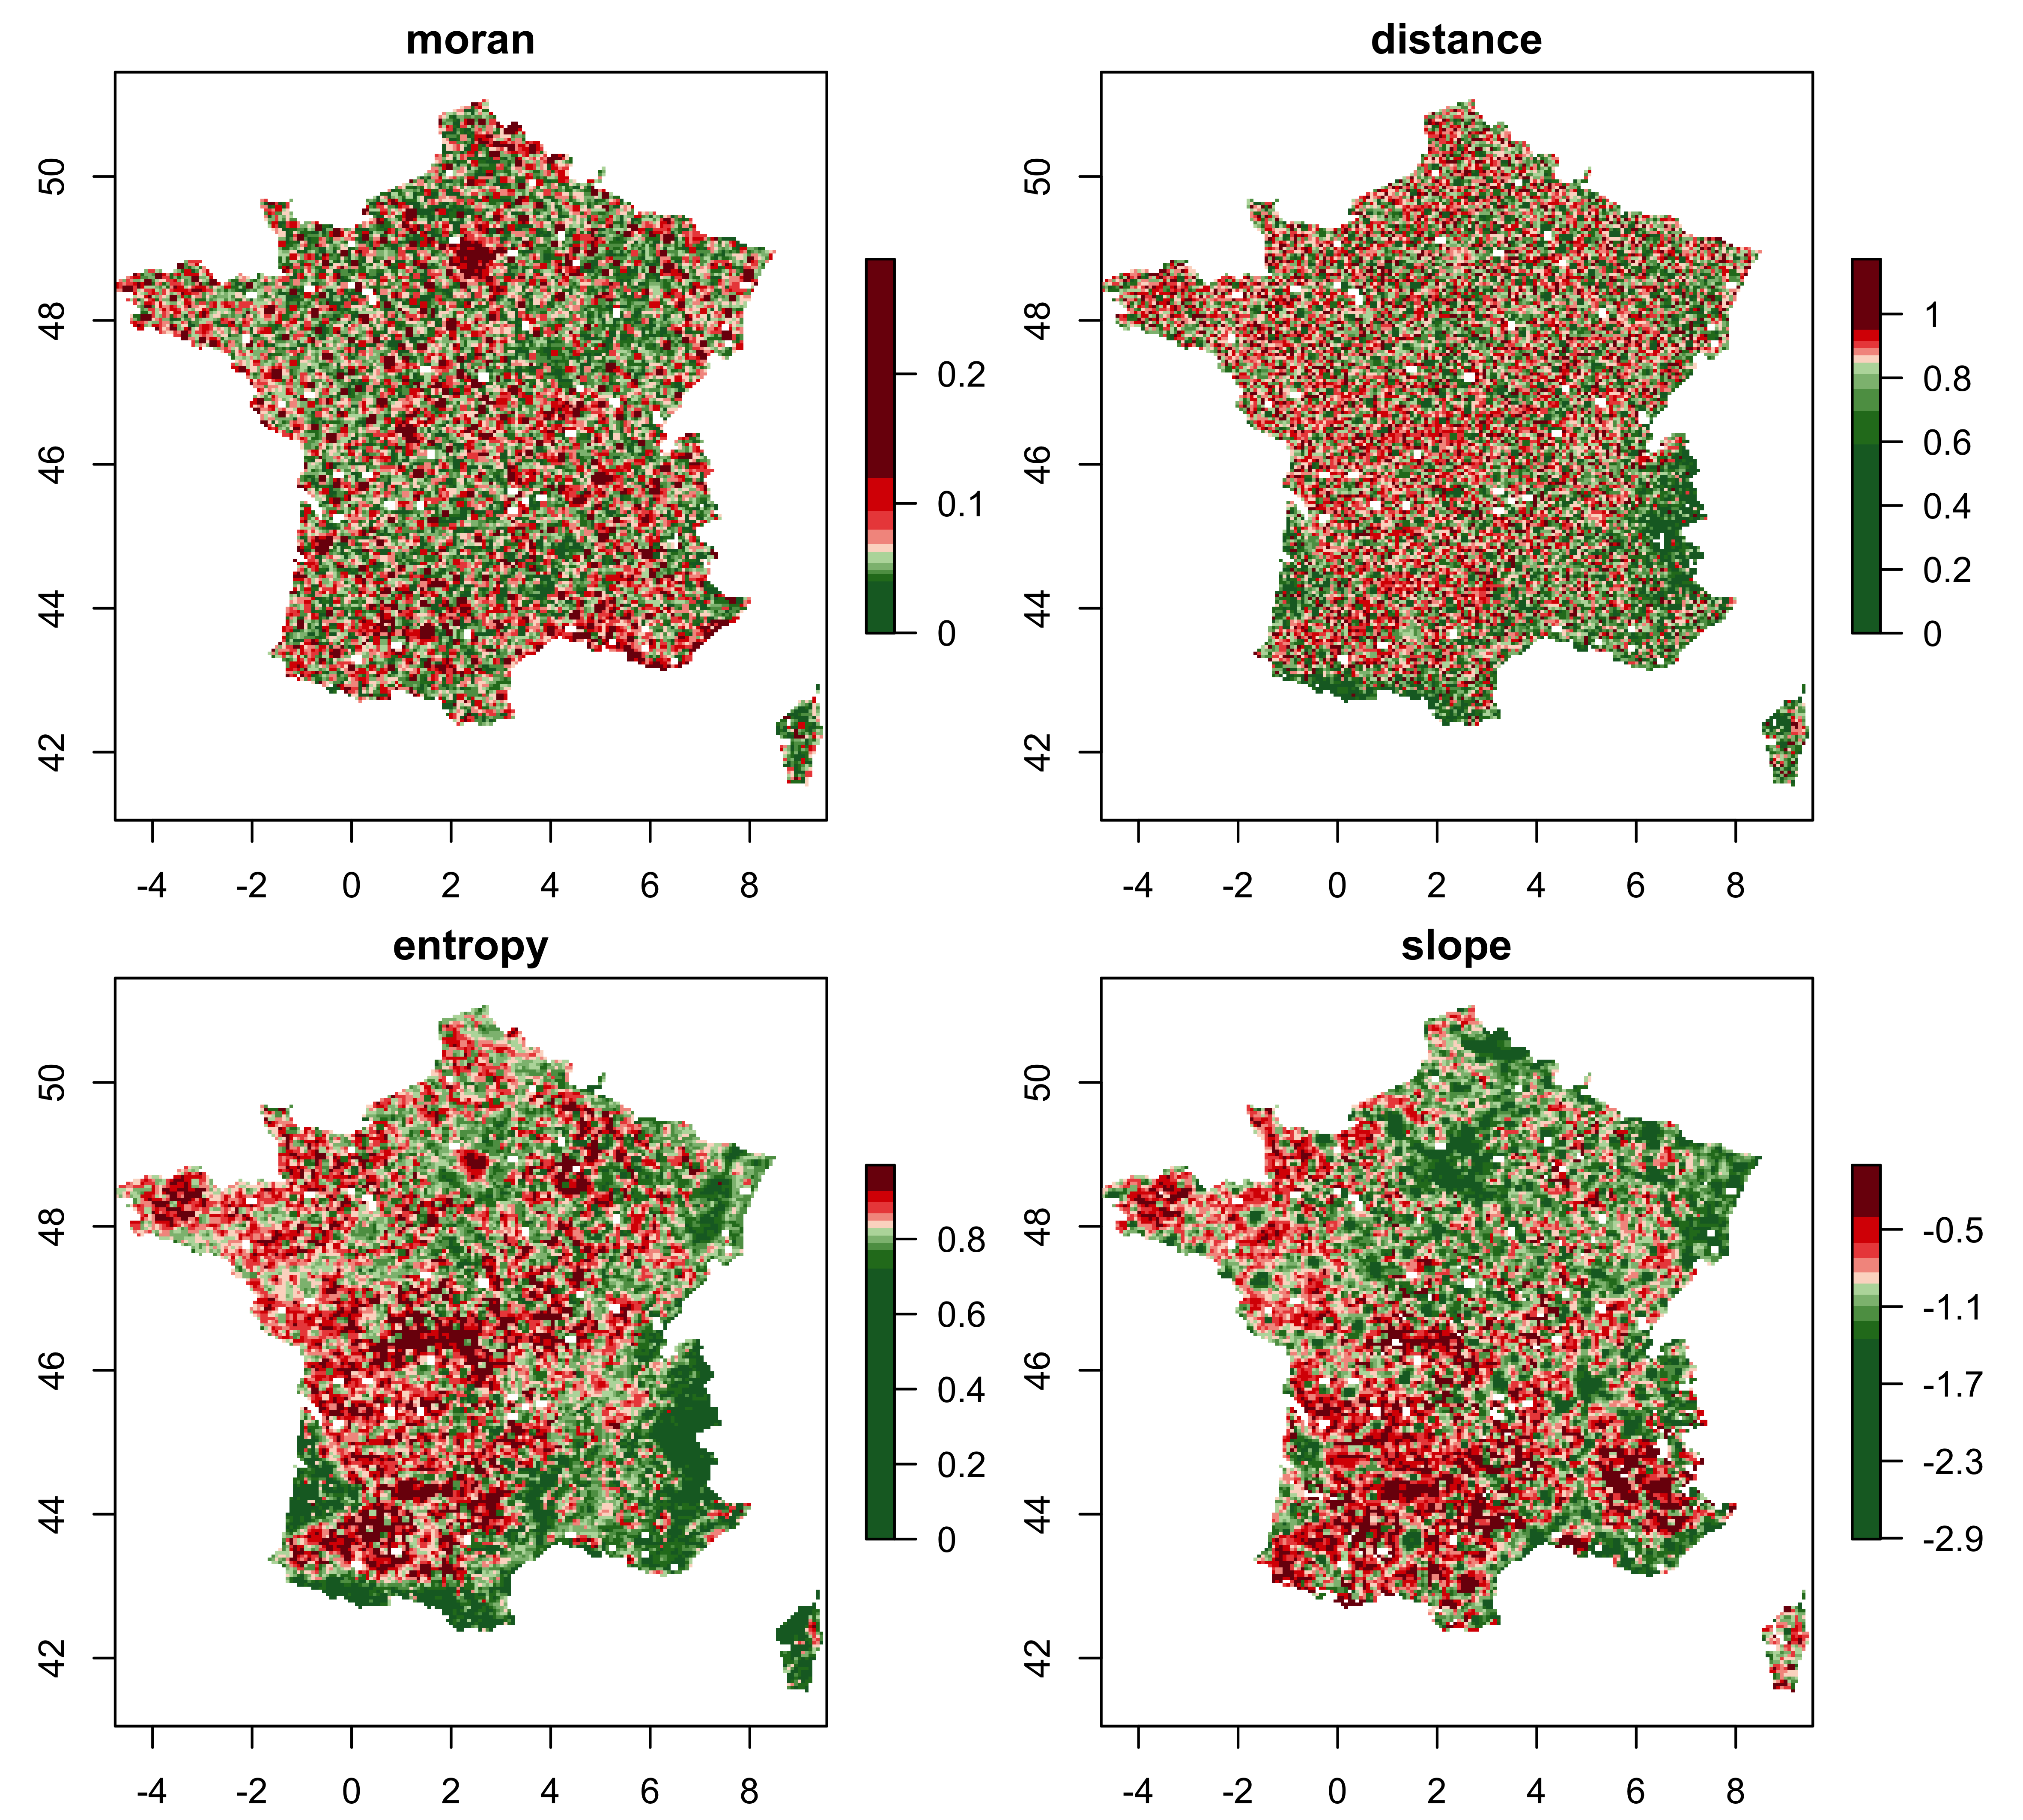
\includegraphics[width=\textwidth]{figures/density_indics_morpho_discrquantiles}
\column{0.3\textwidth}
\centering
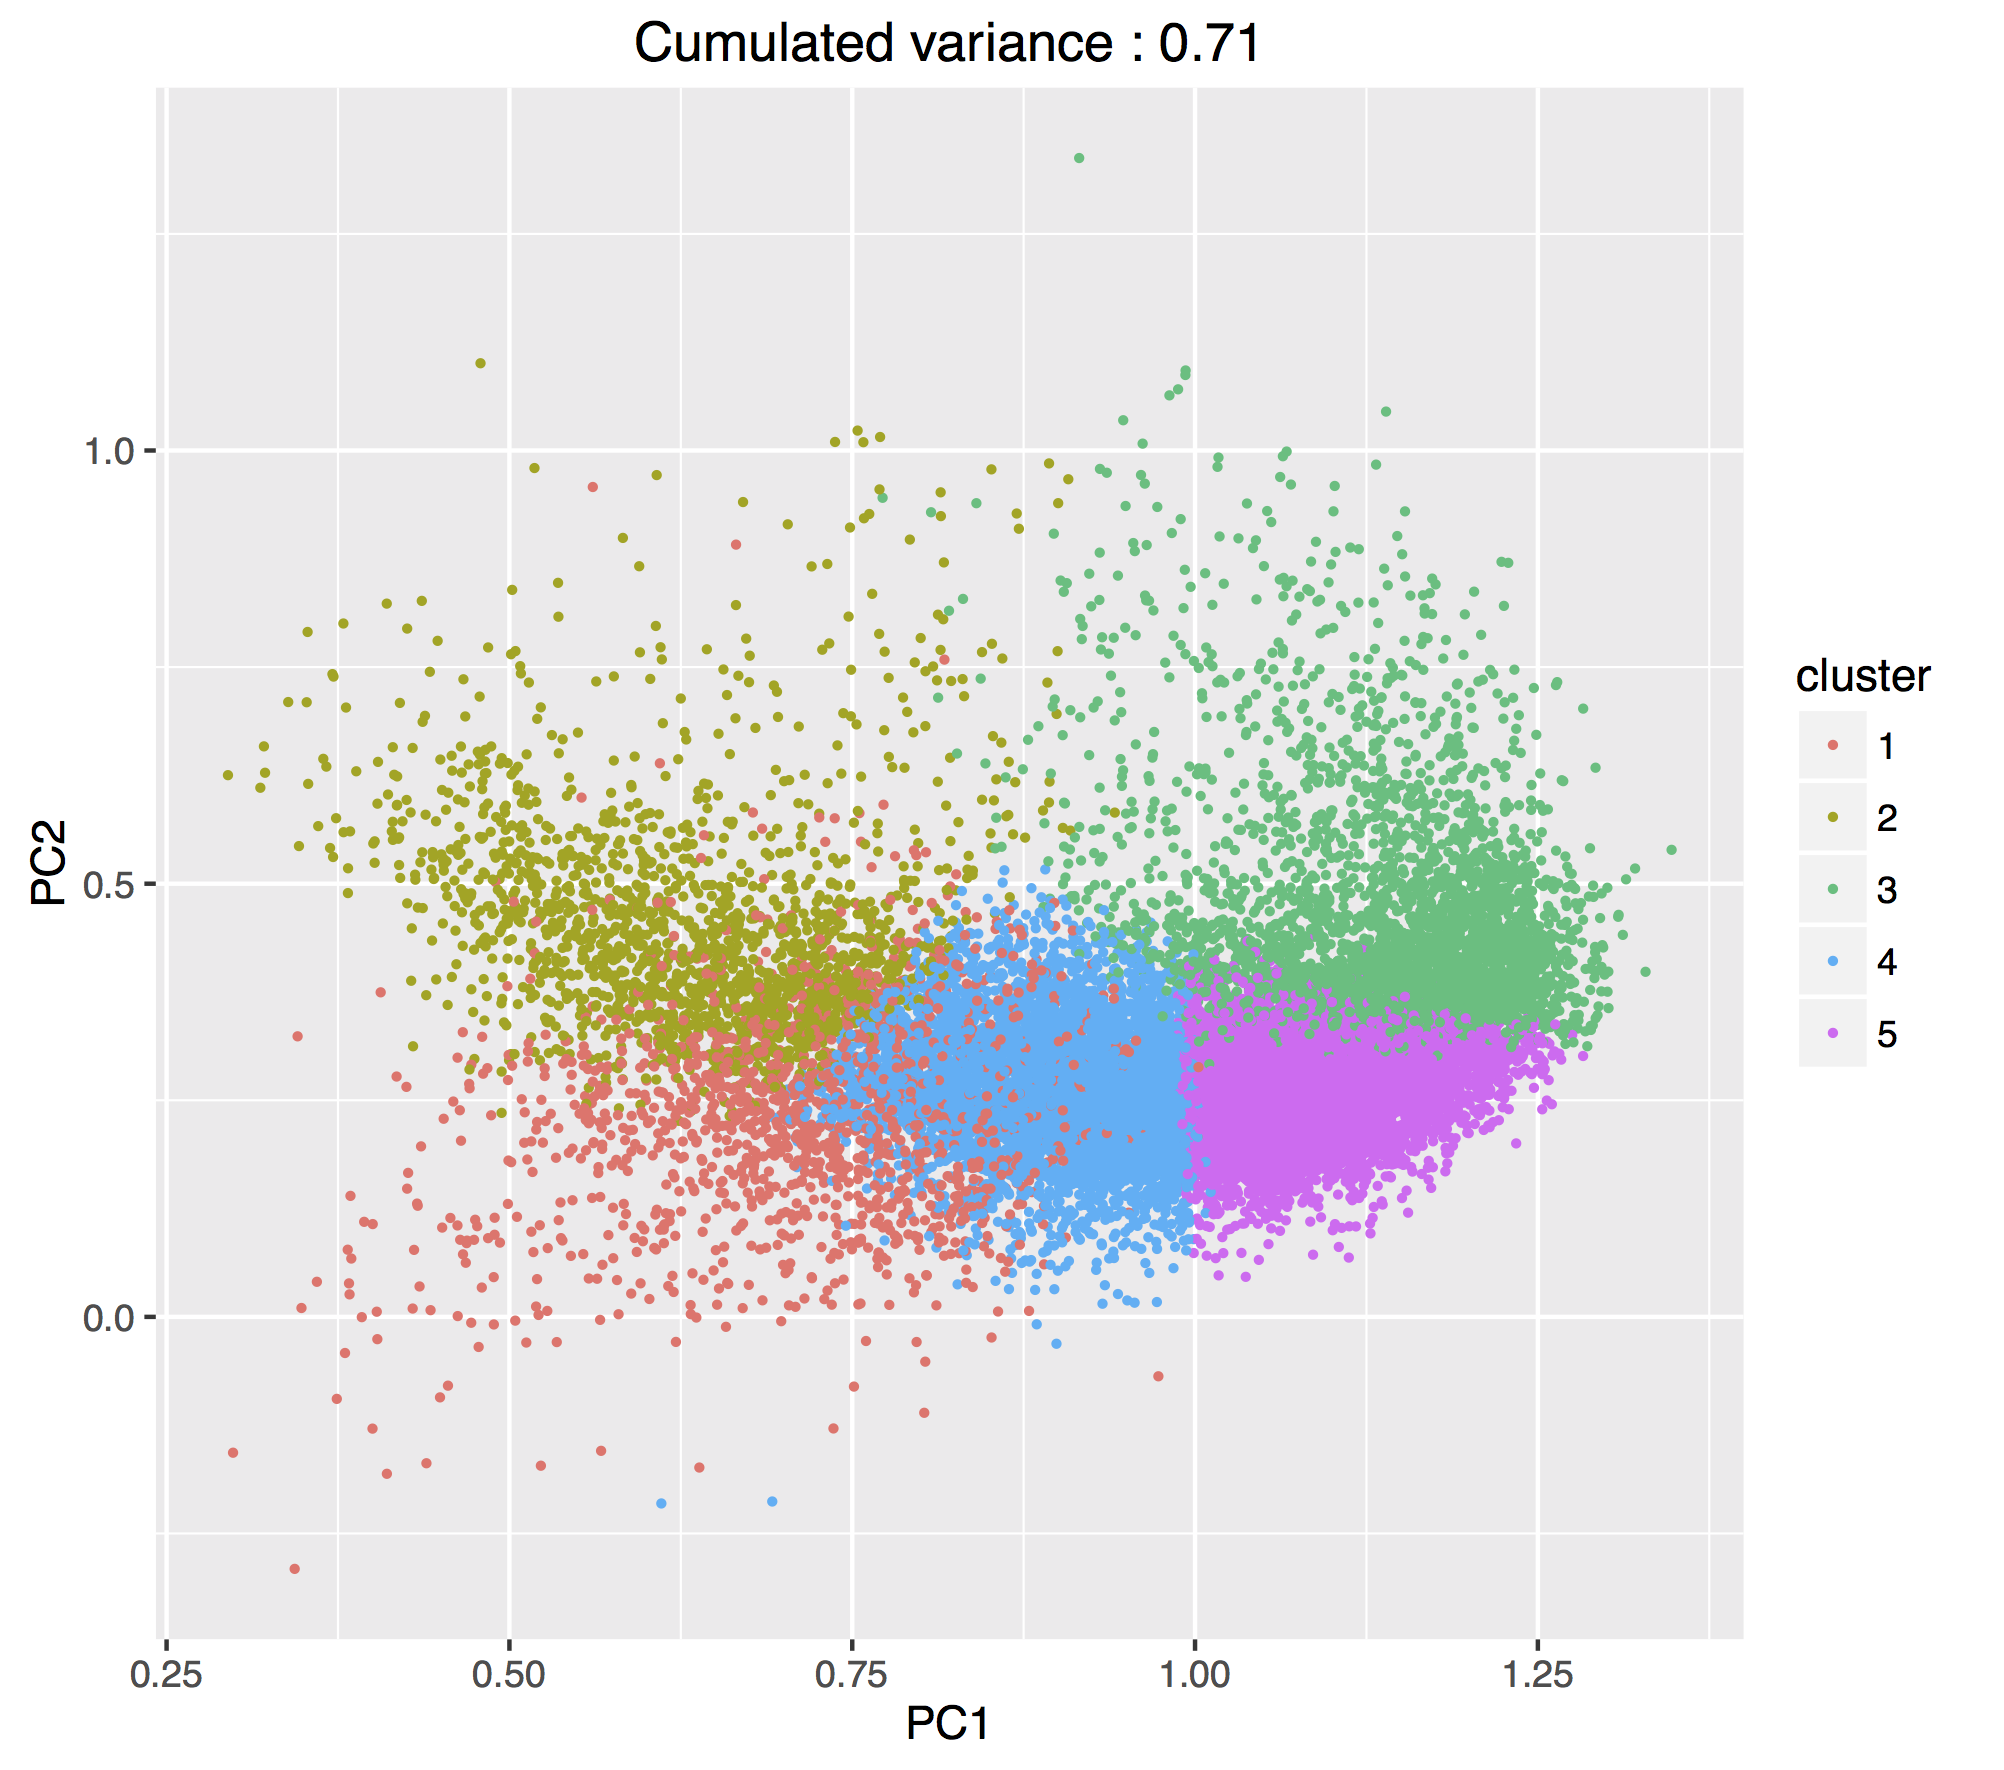
\includegraphics[width=\textwidth]{figures/density_cluster_pca_k5_morpho}\\
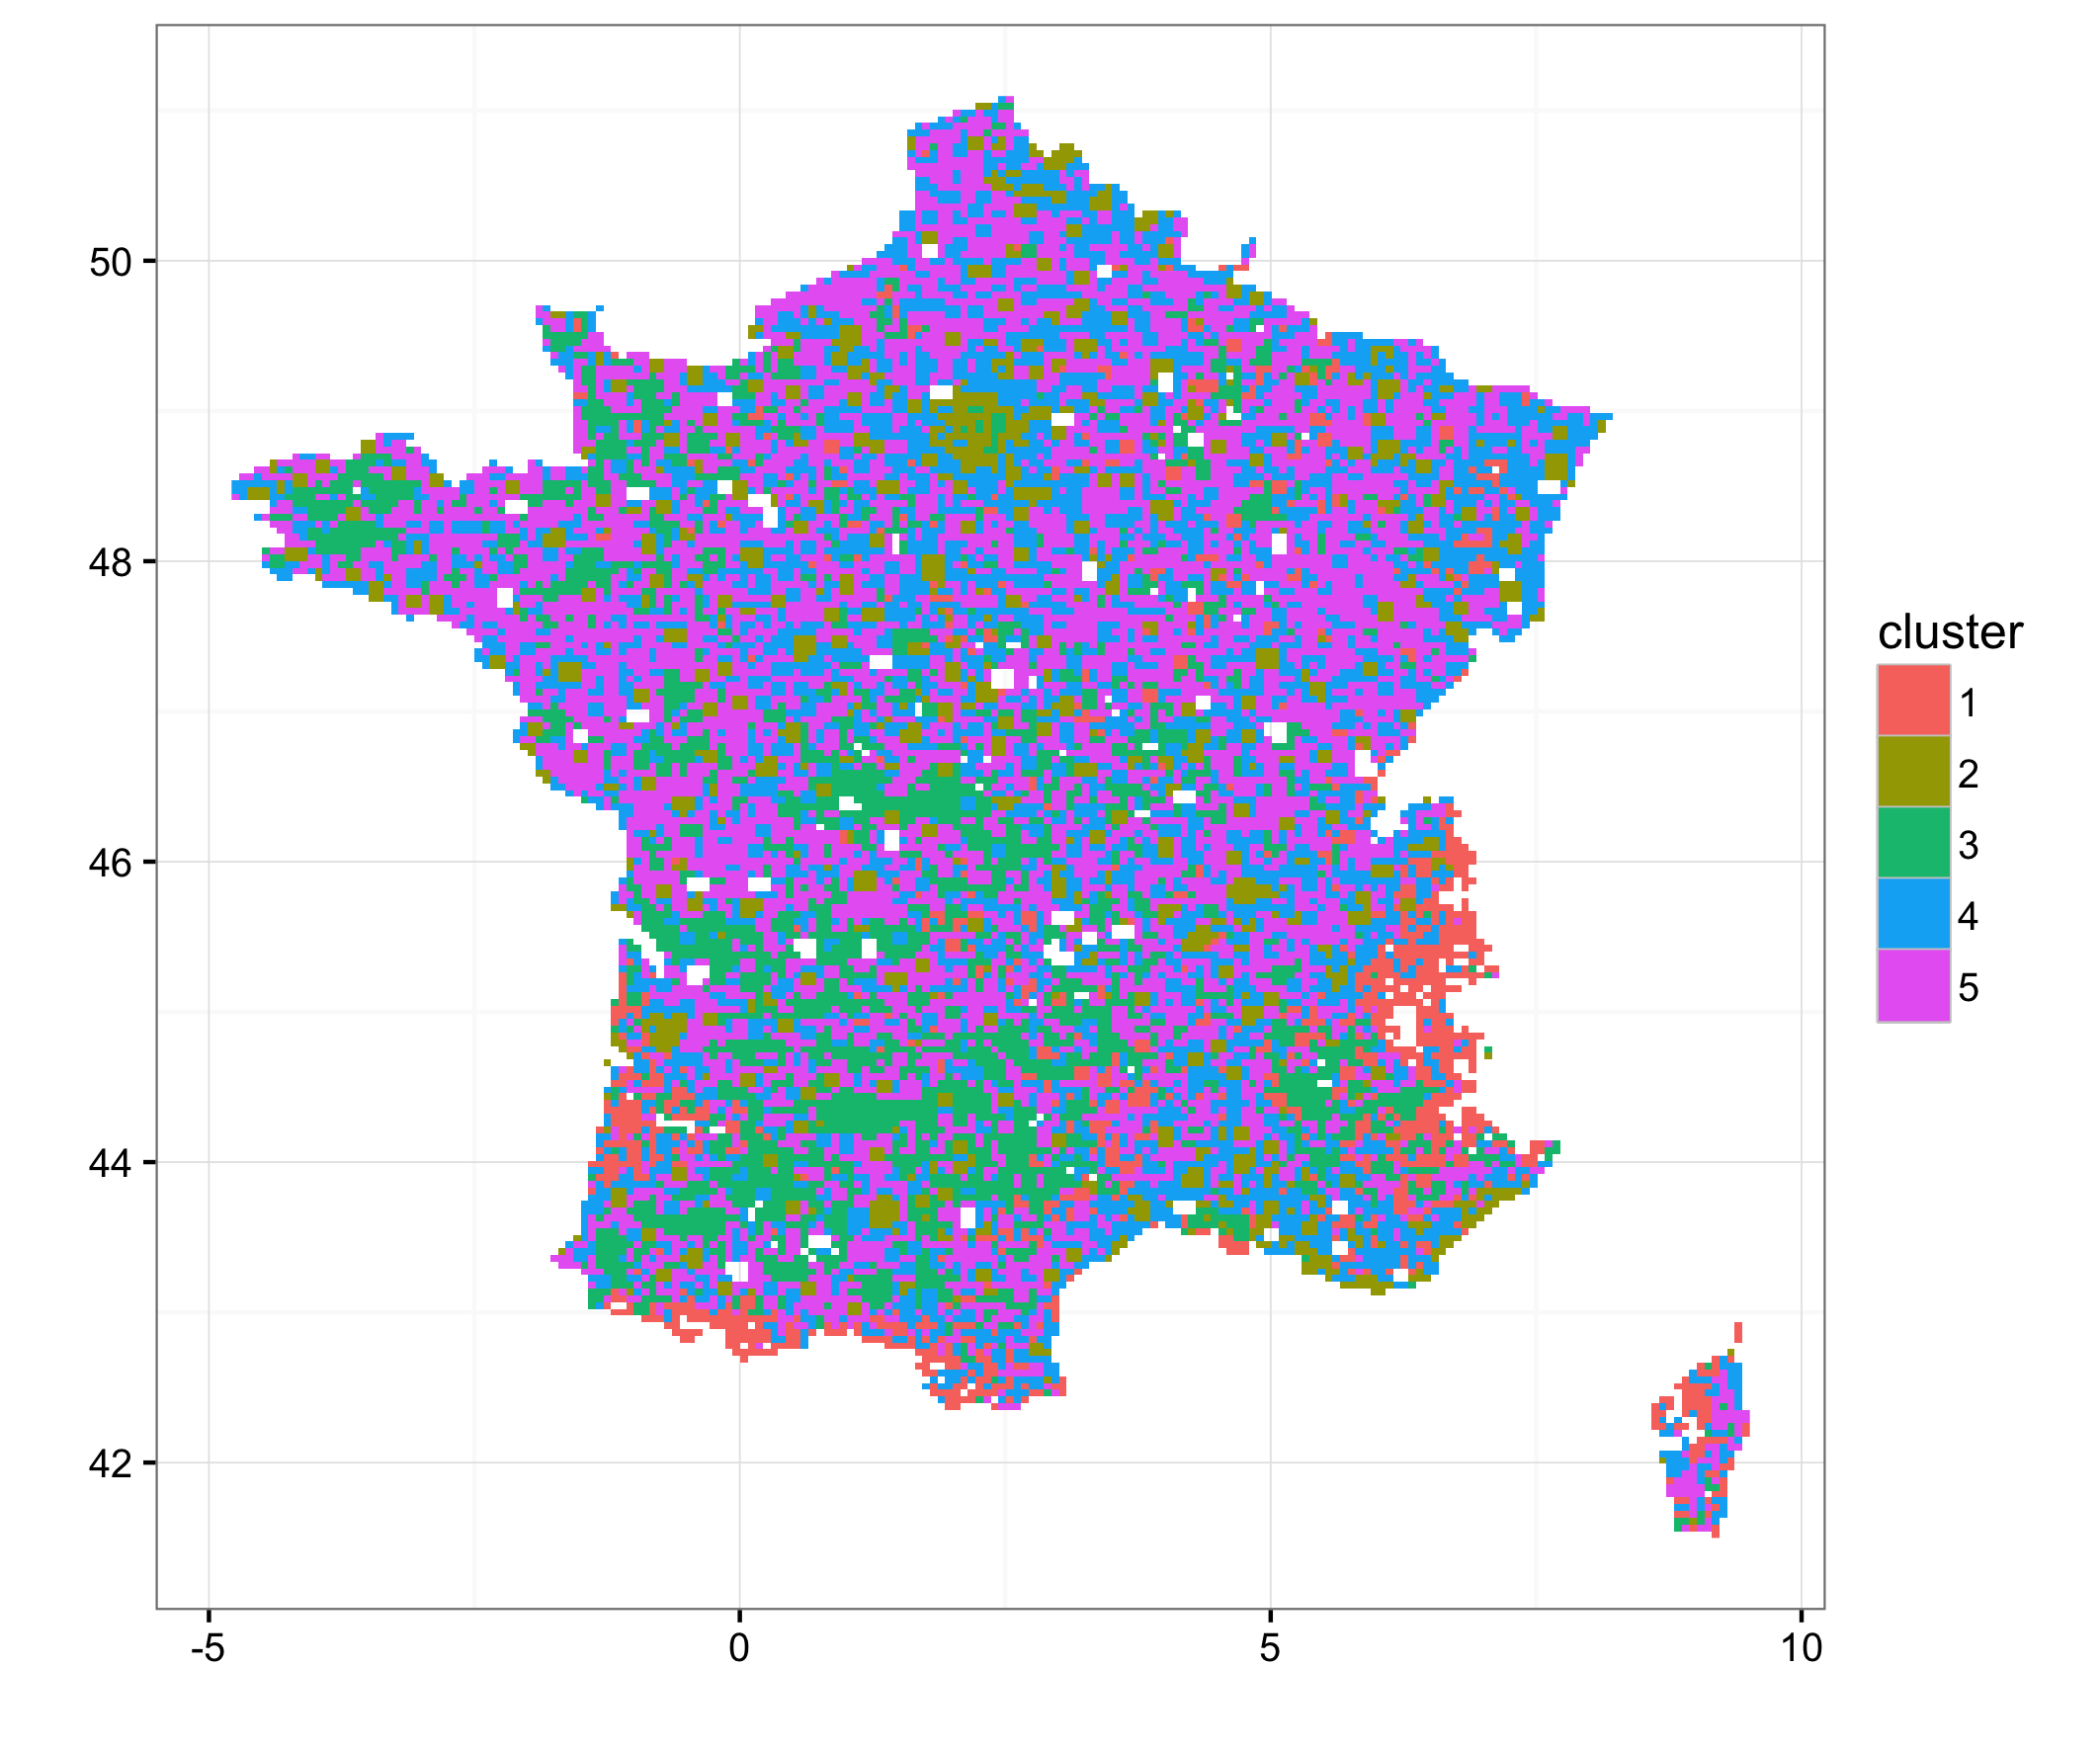
\includegraphics[width=\textwidth]{figures/density_cluster_map_k5_morpho}
\end{columns}

\justify

\footnotesize\textit{Computation of morphological indicators on population density data for Europe (shown here on France), morphological classification.}

}






\sframe{Model classification : PDE}{

% derived PDE

The one-dimensional model verifies the PDE :

\begin{equation}\label{eq:pde}
\begin{split}
\delta t \cdot \frac{\partial p}{\partial t} \textrm{ = } \frac{N_G \cdot p^{\alpha}}{P_{\alpha}(t)} \textrm{ + } \frac{\alpha \beta \left(\alpha - 1\right) \delta x^2}{2}\cdot \frac{N_G \cdot p^{\alpha-2}}{P_{\alpha}\left(t\right)} \cdot \left(\frac{\partial p}{\partial x}\right)^2\\
\textrm{ + } \frac{\beta \delta x^2}{2} \cdot \frac{\partial^2 p}{\partial x^2} \cdot\left[ 1 \textrm{ + } \alpha \frac{N_G p^{\alpha - 1}}{P_{\alpha(t)}} \right]
\end{split}
\end{equation}

}


\sframe{Stationary behavior of 1D model}{
\centering
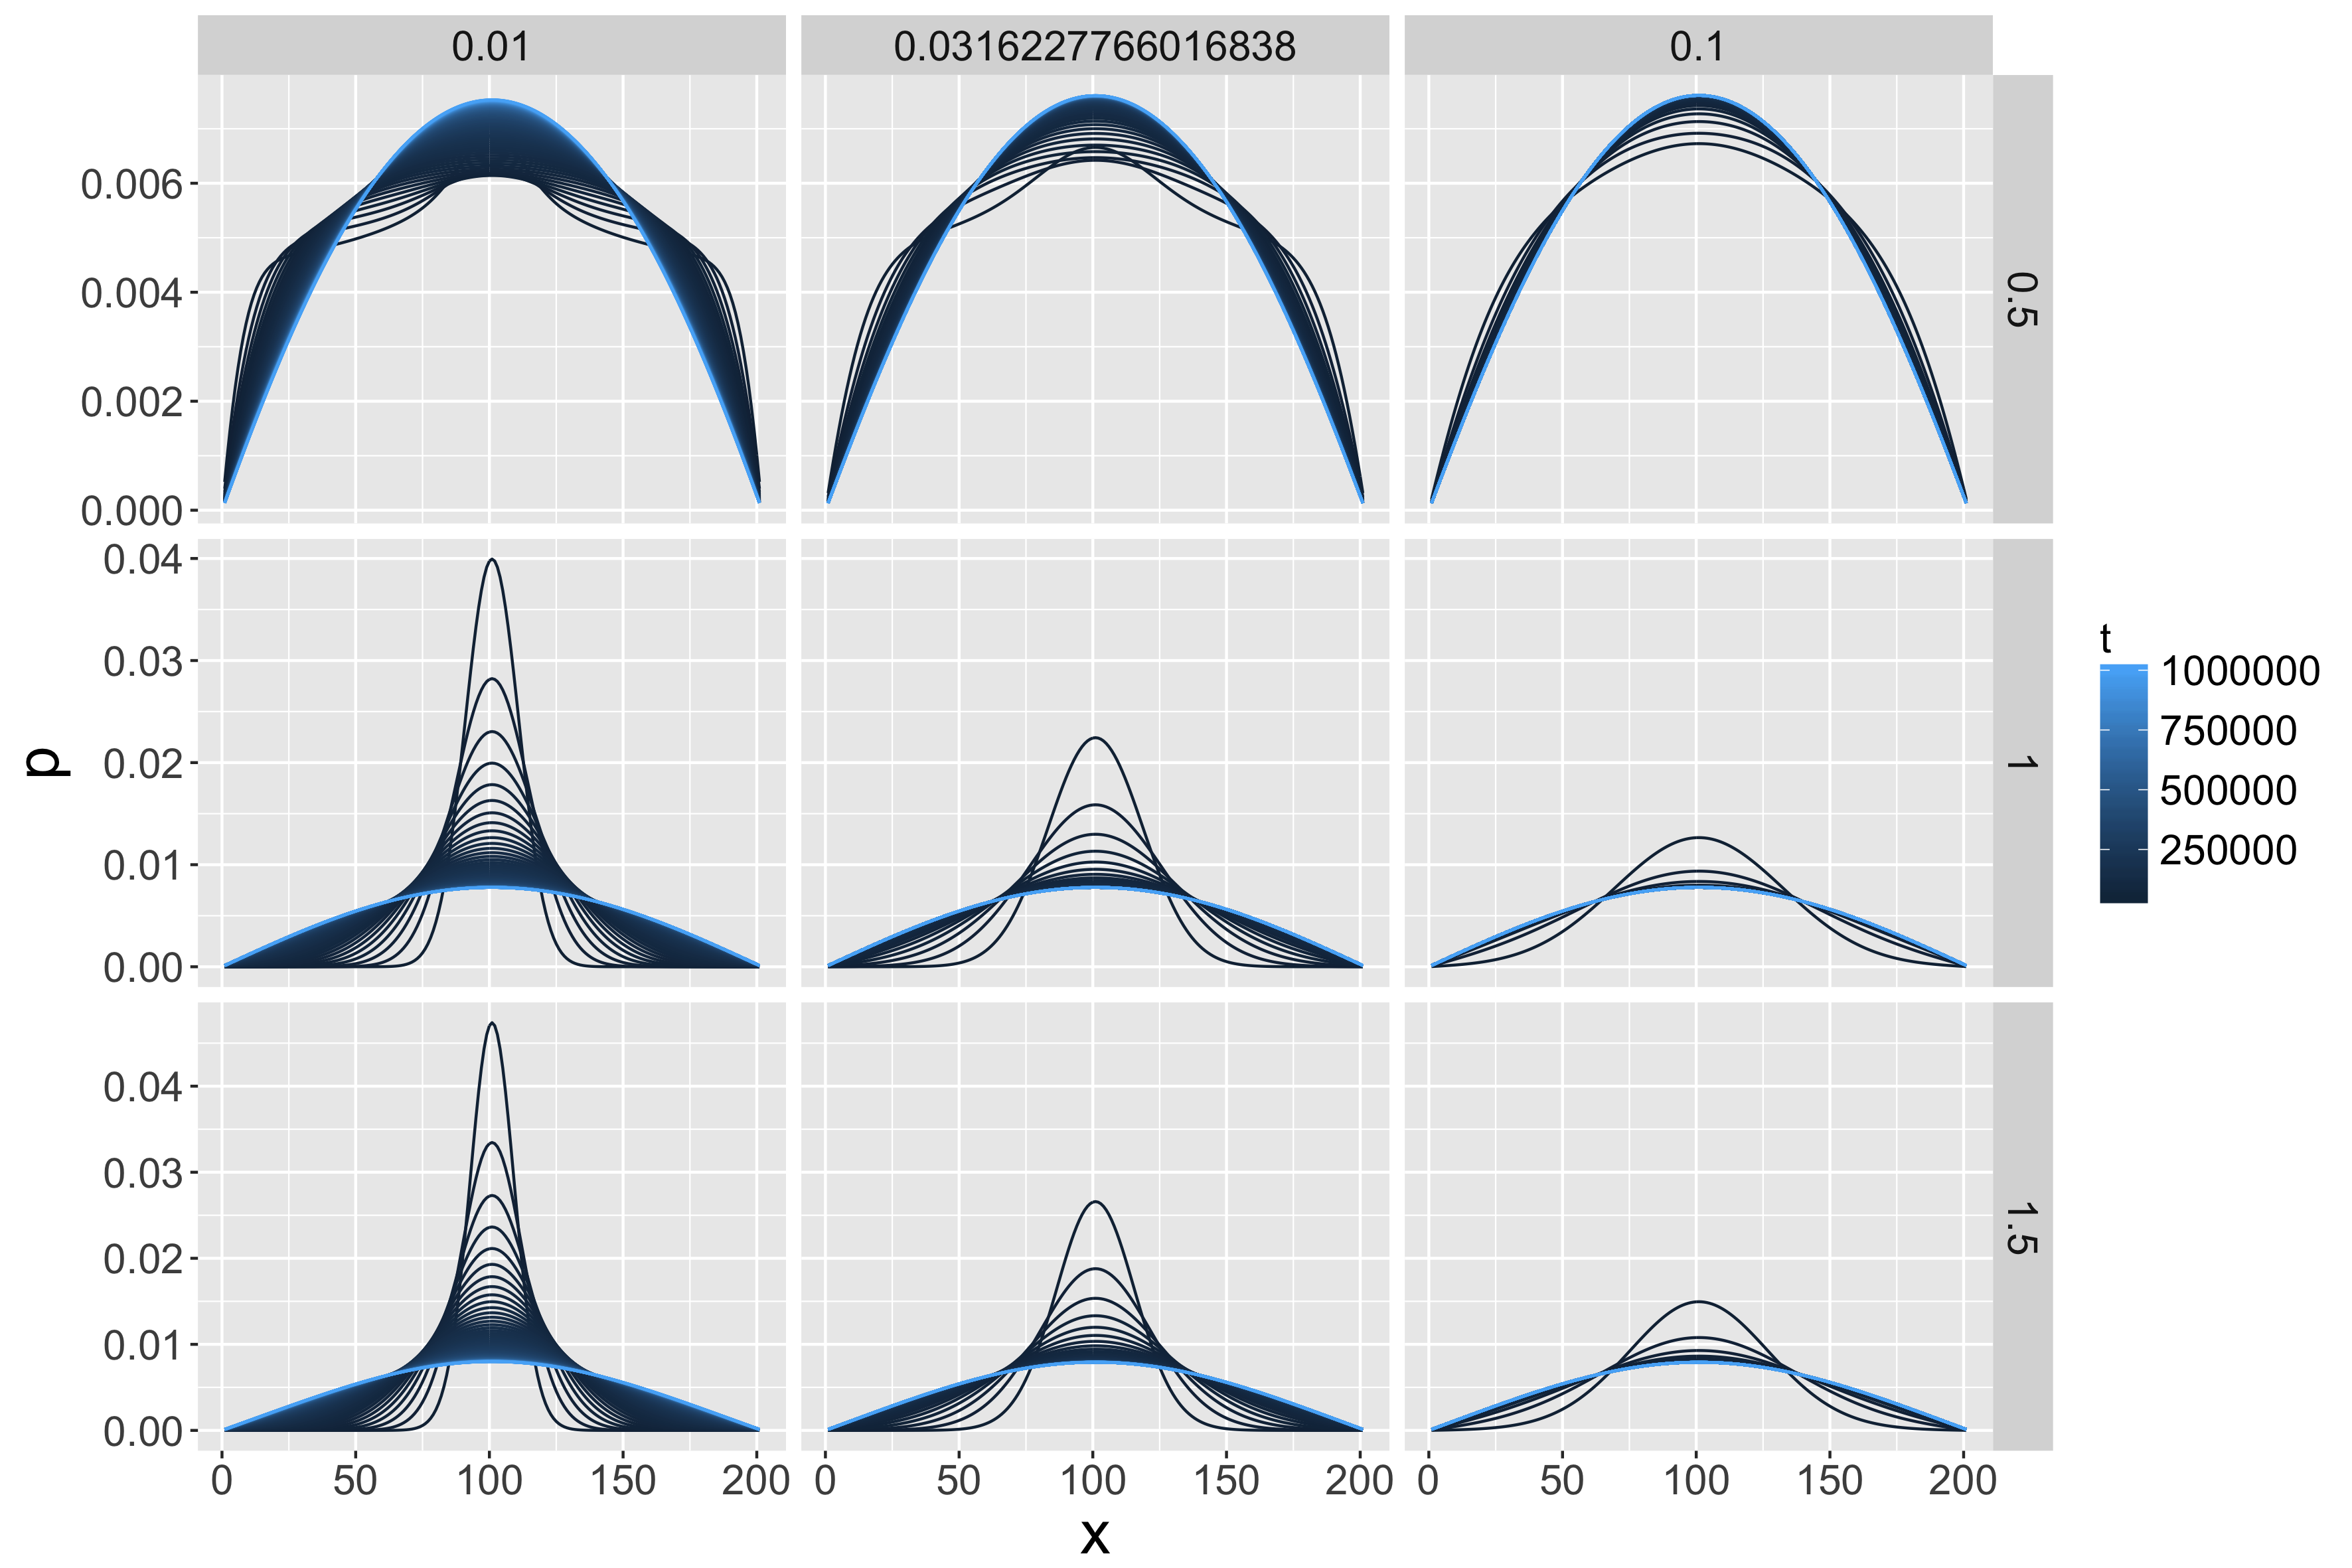
\includegraphics[width=\textwidth]{figures/density_stationary}
}

\sframe{Stationary behavior of 1D model}{
\centering
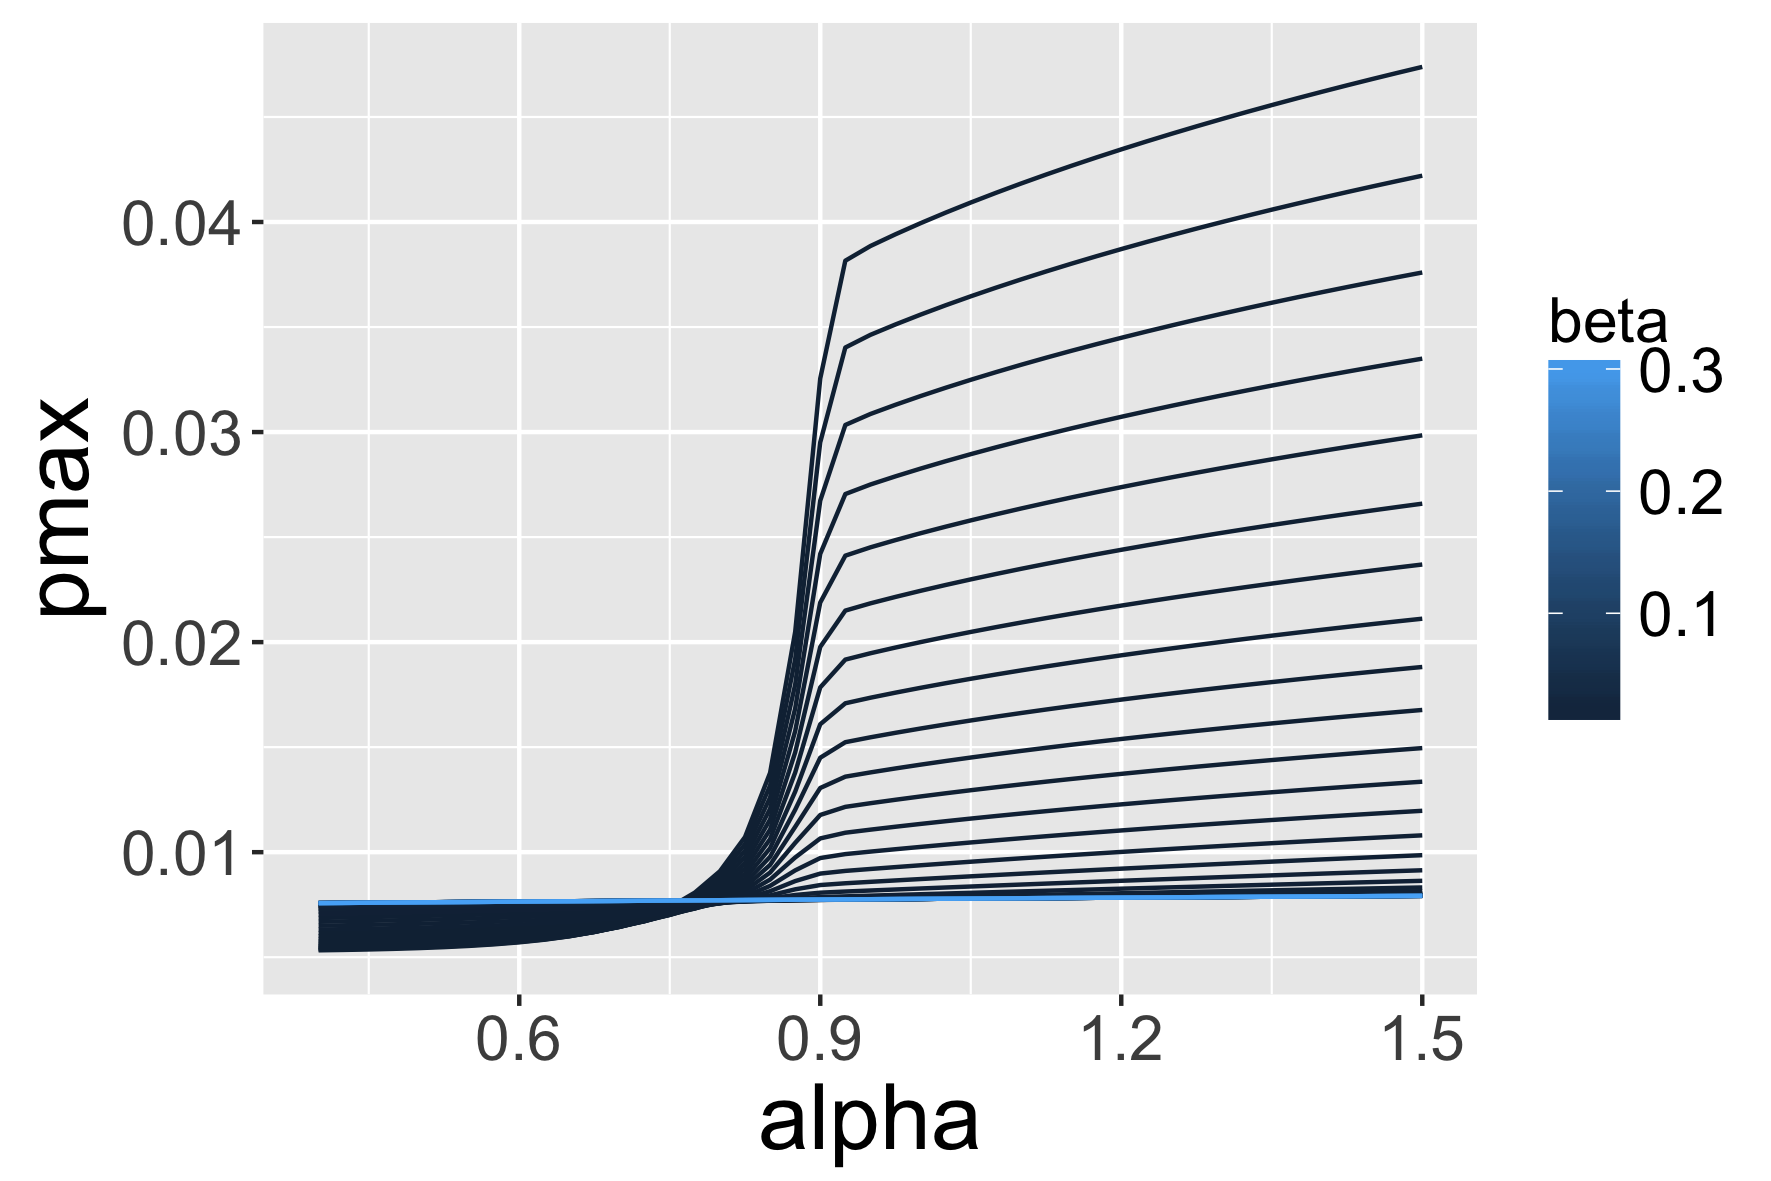
\includegraphics[width=0.48\textwidth]{figures/density_pmax_alpha}
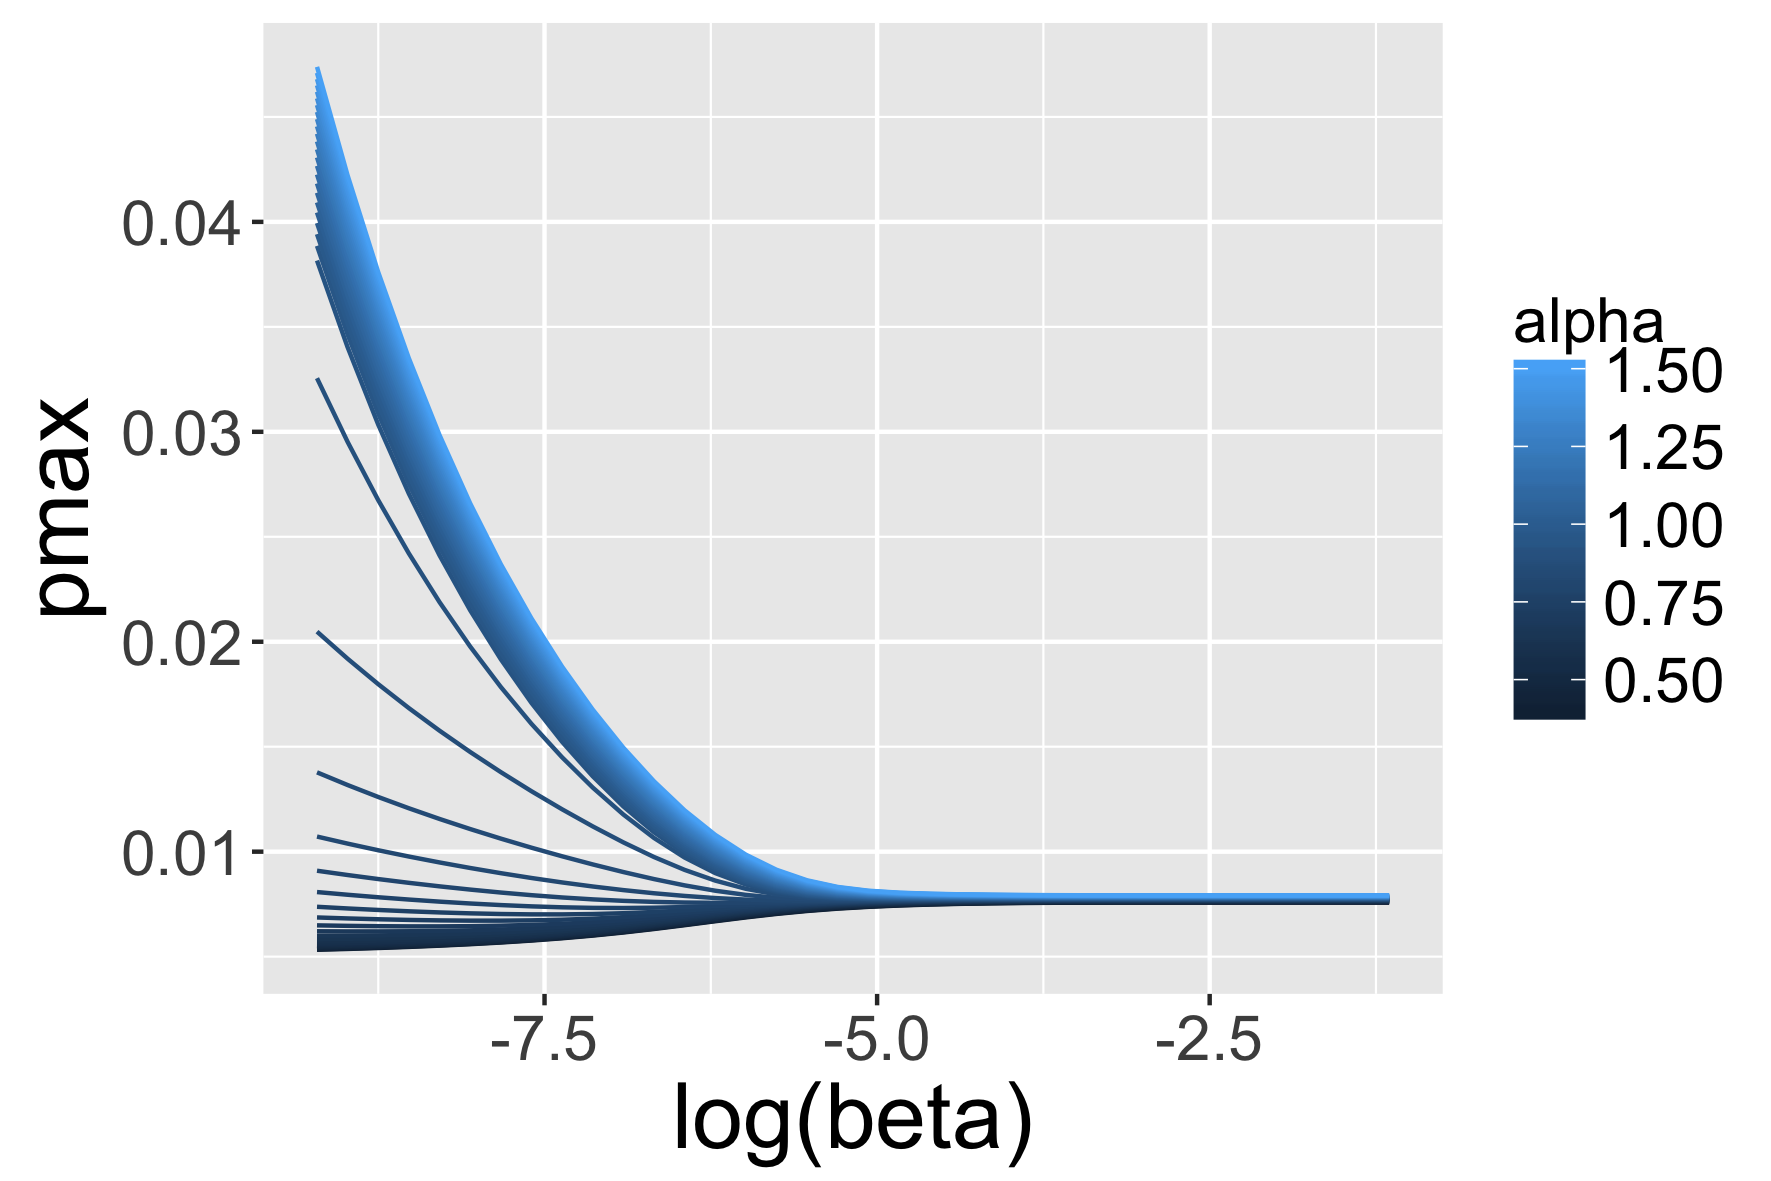
\includegraphics[width=0.48\textwidth]{figures/density_pmax_logbeta}

}





\sframe{Model behavior : Convergence}{

Large number of repetitions show good convergence properties

% hist examples

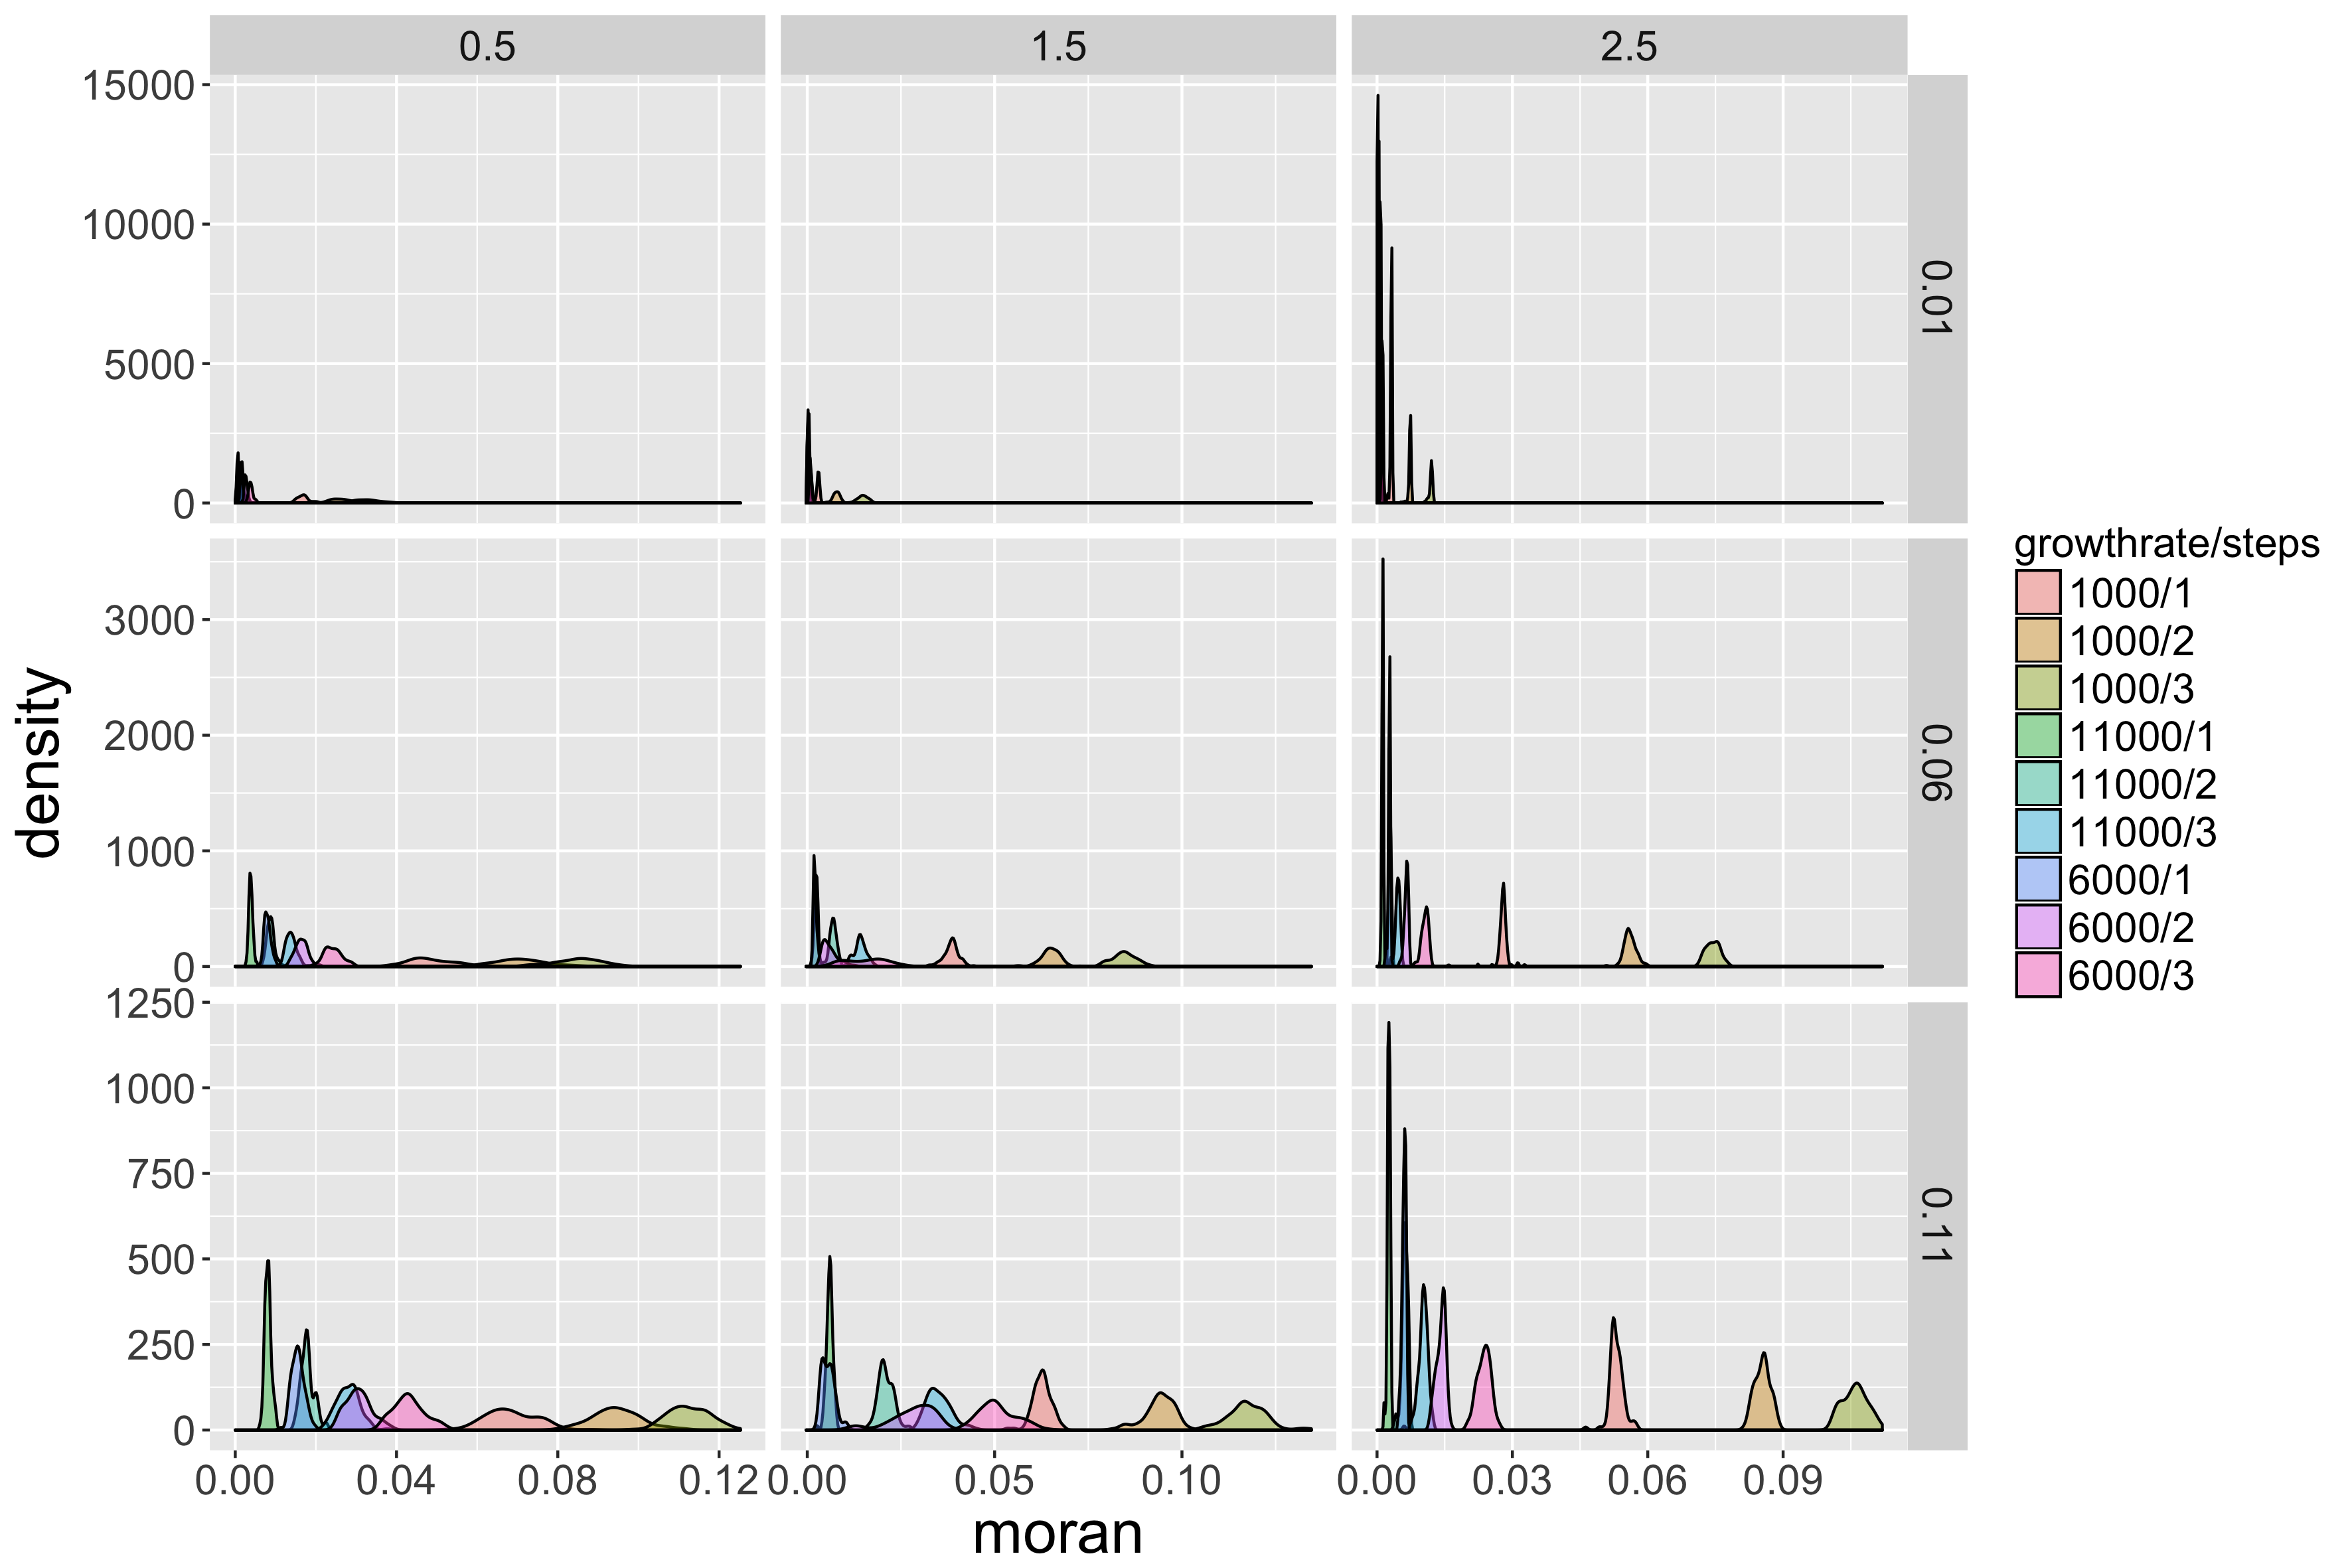
\includegraphics[width=0.5\textwidth]{figures/density_hist_moran}
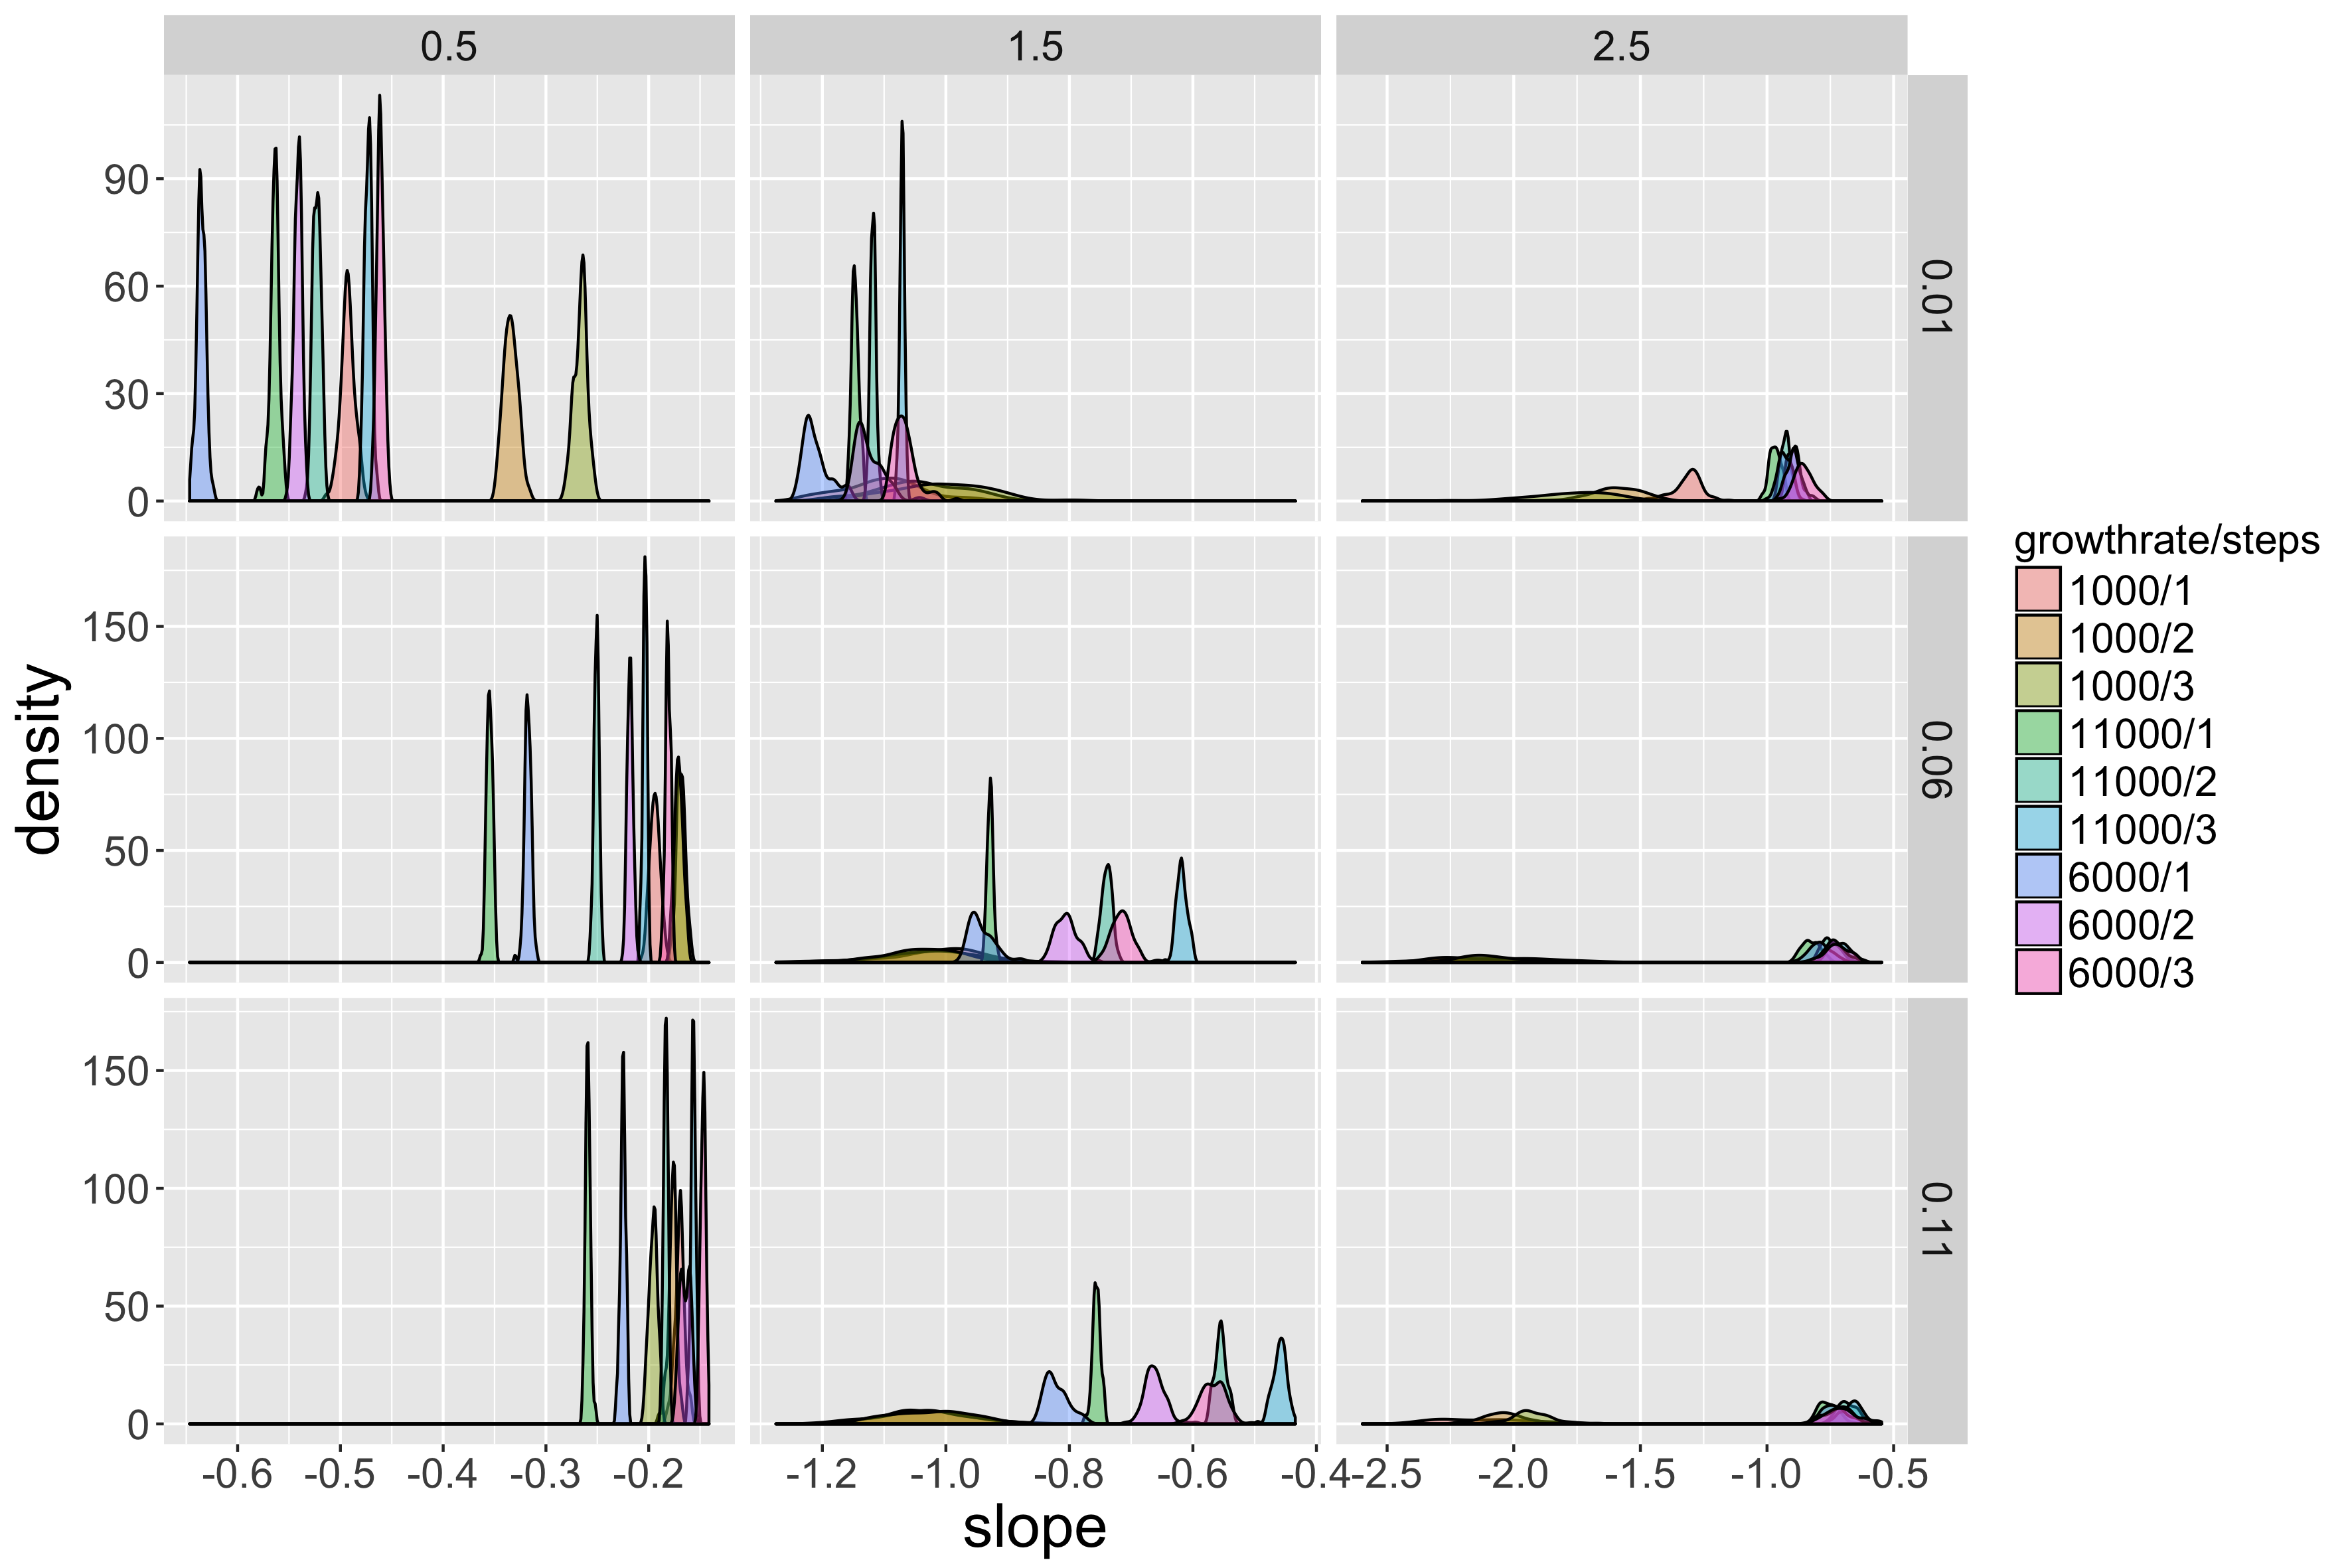
\includegraphics[width=0.5\textwidth]{figures/density_hist_slope}

}


\sframe{Model behavior}{


\includegraphics[width=0.5\textwidth]{figures/density_pc_colalpha}
\includegraphics[width=0.5\textwidth]{figures/density_pc_colbeta}

}


\sframe{Empirical indicators computation}{

$\rightarrow$ Eurostat population density raster (100m, simplified at 500m resolution)

\medskip

$\rightarrow$ Overlapping (10km offset) squares of 50km side : equivalent to smoothing, removes window shape effect. Not very sensitive to window size (tested with 30km and 100km)

\medskip

$\rightarrow$ Indicators computed using Fast Fourier Transform Convolution

\medskip

$\rightarrow$ Classification using repeated k-means ; number of clusters taken at transition in clustering coefficient.

}

\sframe{Model calibration: all indicators}{

\centering
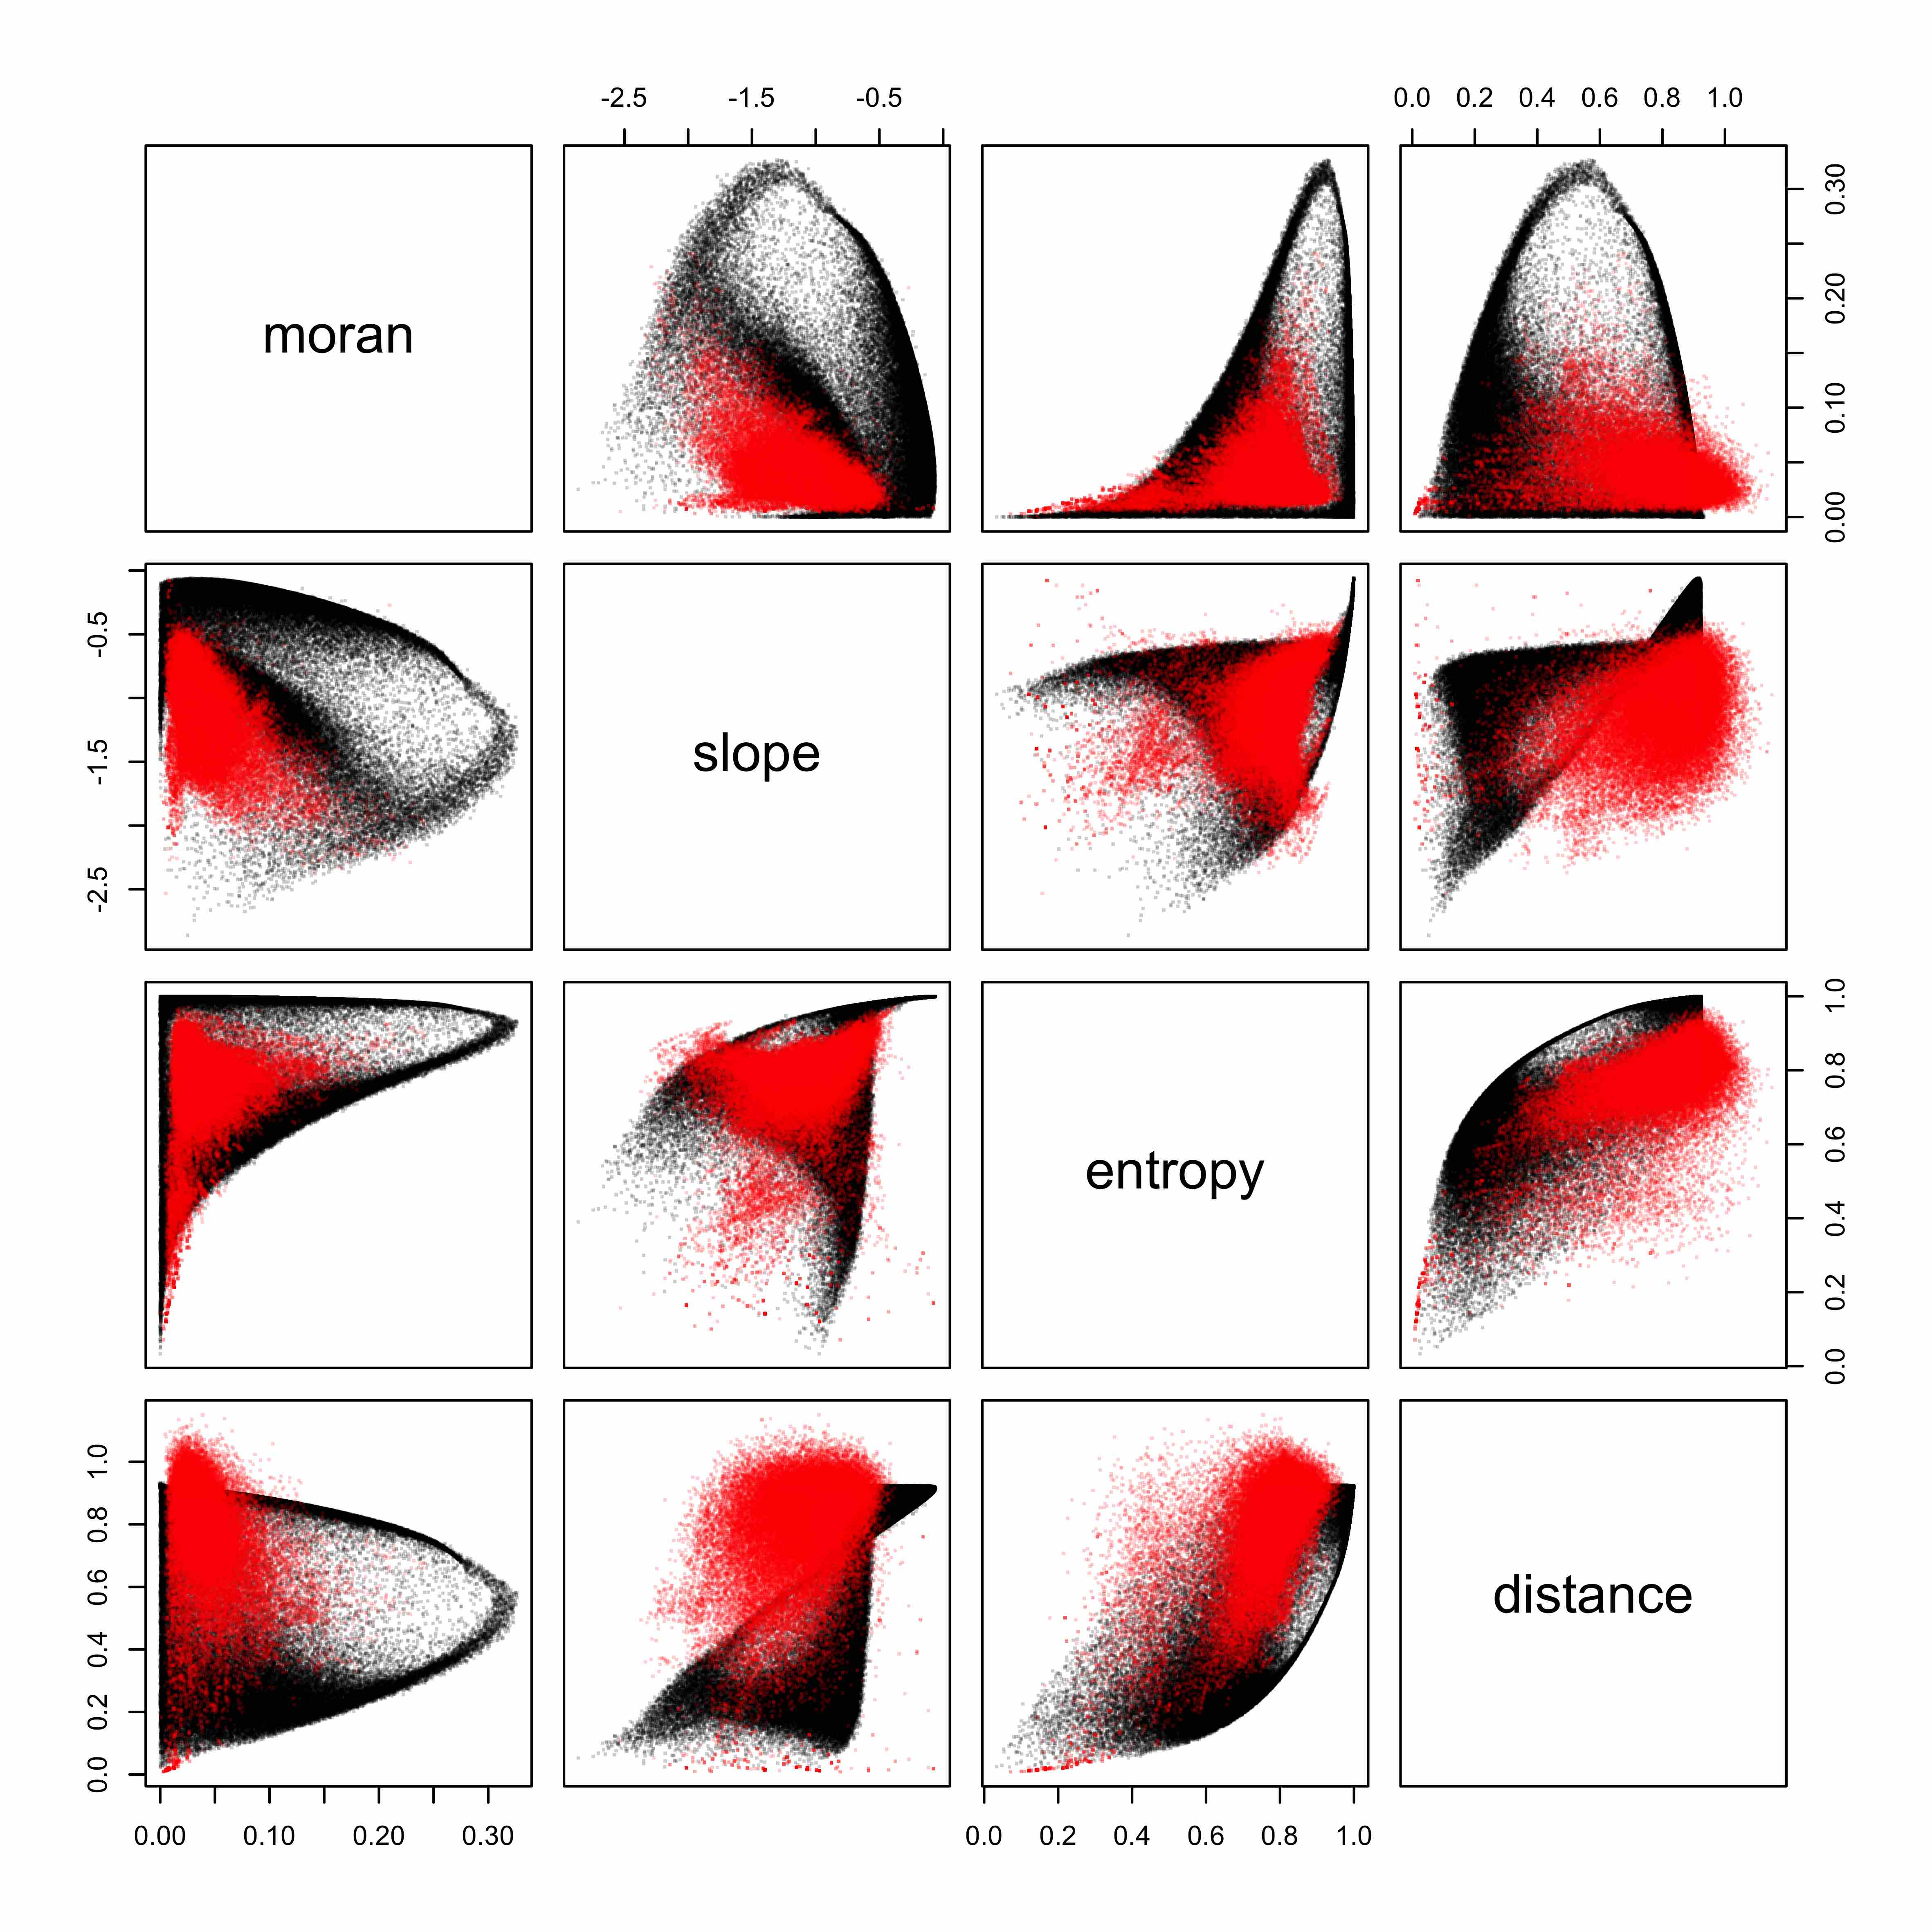
\includegraphics[width=0.65\textwidth]{figures/density_scatter}

}




\sframe{Model Targeted Exploration}{

\centering

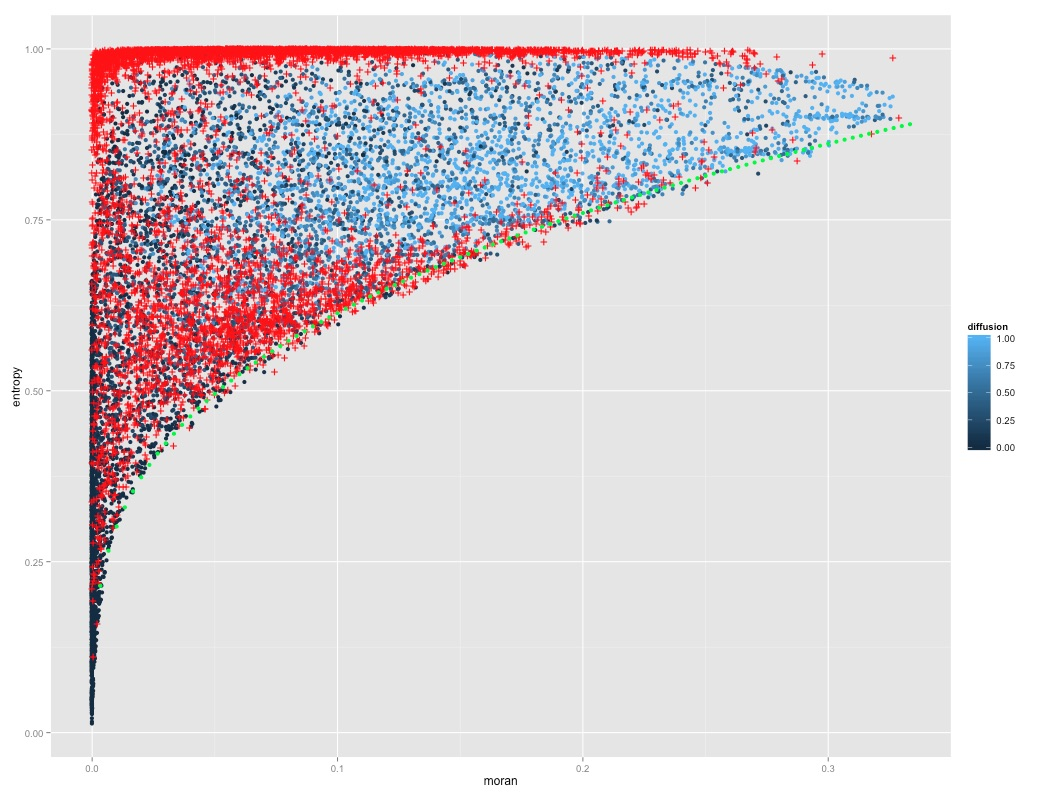
\includegraphics[width=0.8\textwidth]{figures/density_Fig6}

\footnotesize\textit{Potentialities of targeted model explorations: here feasible space using Pattern Space Exploration algorithm \cite{10.1371/journal.pone.0138212}.}

}




\sframe{Defining Morphogenesis}{

% precise notions and defs

\justify

\textit{Proposition of an interdisciplinary definition}

\bigskip




\textbf{Meta-epistemological framework of imbricated notions:}

Self-organization $\supsetneq$ Morphogenesis $\supsetneq$ Autopoiesis $\supsetneq$ Life


\bigskip

\textbf{Properties:}

\begin{itemize}
\item Architecture links form and function
\item Emergence strength~\cite{bedau2002downward} increases with notion depth, as bifurcations~\cite{thom1974stabilite}
\end{itemize}

\bigskip

\textbf{Definition of Morphogenesis :} \textit{Emergence of the form and the function in a strongly coupled manner, producing an emergent architecture \cite{doursat2012morphogenetic}}



}





%%%%%%%%%%%%%%%%%%%%%
\begin{frame}[allowframebreaks]
\frametitle{References}
\bibliographystyle{apalike}
\bibliography{biblio}
\end{frame}
%%%%%%%%%%%%%%%%%%%%%%%%%%%%





%\sframe{What is Morphogenesis ? Examples}{

% illustrations : ants, geomorphology, neurons, self-assembly ; ARBOTRON ; paper nature aile avion
% all from netlogo library ? would be nice illustration of generative nature


% remark : do not put classical biological example to show how it has percolated to other fields
%\vspace{-0.3cm}
%\includegraphics[width=\textwidth,height=0.82\textheight]{figures/intro_examples}

%\justify

%\vspace{-0.5cm}

%\footnotesize\textit{Sources (in order by column). Ants, Erosion, Game of Life: NetLogo Library; Arbotron \cite{jun2005formation}; Industrial design \cite{Aage:2017aa}; Swarm chemistry \cite{sayama2007decentralized}}
% sources : ants netlogo ; erosion netlogo ; arbotron 
%  inge : 
%}



\end{document}






